%% Preamble %%
\RequirePackage{fix-cm}
\documentclass[12pt,a4paper,twoside,table]{report}
\usepackage[utf8]{inputenc}
\usepackage[T3,T1]{fontenc}
%\usepackage[english]{babel}

%% FORMAT %%

%Page settings
\topmargin -10mm
\textwidth 160truemm
\textheight 240truemm
\oddsidemargin 0mm
\evensidemargin 0mm

%Header and footer settings
\usepackage{fancyhdr} %Header package
\pagestyle{fancy}
\fancyhead{}
\fancyhead[LE]{\leftmark}
\fancyhead[RO]{\rightmark}
\fancyfoot{}
\fancyfoot[LE,RO]{\thepage}
\renewcommand{\headrulewidth}{0.3pt} %Set header rule width 


%% NEW COMMANDS/SYMBOLS %%

%% New command for horizontal lines in matrices in TikZ diagrams
% \mhline[<style>]{<matrix name>}{<column number below of the line>}{<number of columns in a row>}
\newcommand\mhline[4][]{%
  \node[fit=(#2-#3-1),inner sep=0pt,outer sep=0pt](R){};
  \foreach \i in {1,...,#4}\node[fit=(R) (#2-#3-\i),inner sep=0pt,outer sep=0pt](R){};
  \draw[#1] (R.north -| #2.west) -- (R.north -| #2.east);
}

%% Create the inverted breve in math mode %%
\DeclareSymbolFont{tipa}{T3}{cmr}{m}{n}
\DeclareMathAccent{\invbreve}{\mathalpha}{tipa}{16}

%% Command and package to make a "formal" environment to have note inside the text.
\usepackage{framed} % for defining framed environment
\newenvironment{formal}{
    \def\FrameCommand{{\color{red}\vrule width 2pt}\hspace{2pt}}
    \MakeFramed{\advance\hsize-\width}
    \vspace{2pt}\noindent\hspace{-7pt}\vspace{3pt}
    }{\vspace{3pt}\endMakeFramed}

%% Get a clear page (for the cover page) %%
\newcommand\blankpage{%
    \null
    \thispagestyle{empty}%
    \addtocounter{page}{-1}%
    \newpage} 

%% FONTS %%

\usepackage{textcomp} % nice greek alphabet
\usepackage{pifont}   % Dingbats
\usepackage{booktabs}
\renewcommand\familydefault{\sfdefault} %Define the font
\usepackage{csquotes} %to avoid probelms with babel in quotes

%% MATH & EQUATIONS %%

\usepackage{amssymb,amsthm}
\usepackage{amsmath}
\usepackage{bm} % bold math
\usepackage{amsfonts} %for bold font in math environement
\usepackage{wasysym} %to have the diameter symbol
\numberwithin{equation}{subsection} %allow equation numbering to be divided by ubsection numbering
\renewcommand{\theequation}{\thesubsection\arabic{equation}} %avoid double dot in the numbering of equation using subsection numbering

%% FIGURES %%

\usepackage{float}
\usepackage[section]{placeins} 
\usepackage[font=small,labelfont={bf}]{caption} %To get caption on subfigures
\usepackage{subcaption} %To get subfigures
\usepackage{rotating} %To have landscape figures
\graphicspath{ {figures/} } %Where the figures are stored
\usepackage{tikz}
\usetikzlibrary{matrix,arrows,decorations.pathmorphing}
\usetikzlibrary{automata,positioning,calc}
\usetikzlibrary{arrows.meta, quotes}

%% TABLES %%
%Command and package for tables
\usepackage{multirow}
\usepackage{array}
\usepackage{threeparttable} % footnotes in tables
\usepackage{cellspace}
    \setlength\cellspacetoplimit{4pt}
    \setlength\cellspacebottomlimit{4pt}
\newcolumntype{C}[1]{>{\centering\arraybackslash}p{#1}} %new type of column

%% APPENDIX %% 

\usepackage[toc,page]{appendix}

%% COVER %%

\usepackage{xcolor} %the table option allows us to alternate coloring in table rows
\usepackage{graphicx,textpos}
\usepackage{helvet}

%Colors for the title page
\definecolor{green}{RGB}{172,196,0}
\definecolor{bluetitle}{RGB}{29,141,176}
\definecolor{blueaff}{RGB}{0,0,128}
\definecolor{blueline}{RGB}{82,189,236}
\setlength{\TPHorizModule}{1mm}
\setlength{\TPVertModule}{1mm}

%% BIBLIOGRAPHY %%
\usepackage[backend=biber,
style=nature,
citestyle=authoryear-comp,
doi=false,
isbn=false,
url=false,
uniquename=init,
giveninits]{biblatex}
\addbibresource{references.bib}
\usepackage[breaklinks,hidelinks]{hyperref} %For url in bibliography

%% EXTRA PACKAGES %%
\usepackage{afterpage} %To get a blank page
\usepackage{lipsum} %To test display
\usepackage{todonotes} %To add to-do notes in the text
\usepackage{enumitem} %To have descriptive lists
\usepackage{chemformula} %To write chemical formulas more easily
\usepackage{pdfpages} % to include pdf as whole pages in the appendix


 %Contains all the packages and specifications

%% Glossary and abreviations %%
%Remove the dot at the end of each abbreviation - nopostdot
%Remove page number at the end of each abbreviation nonumberlist
%Prevent abbreviation grouping - nogroupskip
%Add "List of Abbreviations" to Table of Content - toc

\usepackage[acronym,nopostdot,nogroupskip,nonumberlist,toc,automake]{glossaries} %Load glossaries package

\makeglossaries

% Acronyms
\newacronym{eppn}{EPPN}{European Phenotyping Platforms Network}
\newacronym{EU}{EU}{European Union}
\newacronym{QTL}{QTL}{Quantitative Trait Loci}
\newacronym{PLS}{PLS}{Penalized Least Squares}
\newacronym{SpATS}{SpATS}{Spatial Analysis using Tensor Splines}
\newacronym{inra}{INRA}{Institut National de Recherche Agronomimque (FR) - \textit{National Institute of Agronomical Research}}
\newacronym{VIF}{VIF}{Variance Inflation Factor}
\newacronym{DOE}{DOE}{Design of experiment}

% Definitions
\newglossaryentry{phenotype}{
	name={Phenotype},
	description={Profiling of the structures and functions associated with allelic variants, at the scale of cells, organs, whole plants and canopy}}
	
\newglossaryentry{biostress}{
	name={Biotic stress},
	description={A stress that is caused in plants due to damage instigated by other living organisms, including fungi, bacteria, viruses, parasites, weeds, insects, and other native or cultivated plants.}}
	
\newglossaryentry{abiostress}{
	name={Abiotic stress},
	description={Negative impacts on plants caused by external non-living environmental factors.}}

\newglossaryentry{quantiTL}{
	name={Quantitative trait loci},
	description={Regions of the genome containing one or more genes, associated with variations of a quantitative trait.}
}

\newglossaryentry{screening}{
	name={Screening experiment},
	description={An experiment designed to evaluate the significance of factors and factor-interactions in a model. The factor are usually two-level factor because they are either present in the model or not.}
}

\newglossaryentry{Rs_exp}{
	name={Response surface experiment},
	description={An experiment designed to find the optimal settings for the factors. In this experiment, the significant factors of the model are already determined.}
}

\newglossaryentry{genome}{
	name={Genome},
	description={All of the genes of an individual or organism. All the information that codes for the phenotype that a species displays.}
}

\newglossaryentry{genotype}{
	name={Genotype},
	description={Genetic information, present in the DNA, for a particular trait.}
}

\newglossaryentry{germplasm}{
	name={Germplasm},
	description={Germplasm are living genetic resources such as seeds or tissues that are maintained for the purpose of animal and plant breeding, preservation, and other research uses.}
}

\newglossaryentry{runs}{
	name={Experimental run},
	description={When an experiment is performed a single time in its entirety.}
}

% DEFINITIONS TO INCLUDE:
% - phenotype
% - phenome
% - genotype
% - genome
% - phenomics
% - locus: A locus (plural loci) in genetics is a fixed position on a chromosome, like the position of a gene or a marker (genetic marker).[ (doi:10.1016/0307-4412(95)90659-2)

%\newglossaryentry{}{
%	name={},
%	description={}
%}

\glsaddall  %Adds all the definition to the glossary and all acronyms to the list of abreviations %contains the glossary and abreviations


\begin{document}

%%  Front Cover %%
% Cover 
\thispagestyle{empty}
\newcommand{\form}[1]{\scalebox{1.087}{\boldmath{#1}}}

%
\begin{textblock}{191}(-24,-11)
\colorbox{green}{\hspace{139mm}\ \parbox[c][18truemm]{52mm}{\textcolor{white}{FACULTY OF SCIENCE}}}
\end{textblock}
%
\begin{textblock}{70}(-18,-19)
\textblockcolour{}
\includegraphics*[height=19.8truemm]{LogoKULeuven}
\end{textblock}
%
\begin{textblock}{160}(-6,63)
\textblockcolour{}
\vspace{-\parskip}
\flushleft
\fontsize{40}{42}\selectfont \textcolor{bluetitle}{Comparison of statistical methods and designs for a high throughput phenotyping experiment}\\[1.5mm]
%\fontsize{20}{22}\selectfont Aeroponics at the UCL
\end{textblock}
%
\begin{textblock}{160}(8,153)
\textblockcolour{}
\vspace{-\parskip}
\flushright
\fontsize{14}{16}\selectfont \textbf{Alexandre BOHYN}
\end{textblock}
%
\begin{textblock}{70}(-6,191)
\textblockcolour{}
\vspace{-\parskip}
\flushleft
Supervisor: Prof. P. Goos\\[-2pt]
\textcolor{blueaff}{KULeuven}\\[5pt]
Co-supervisor: Pr. X Draye\\[-2pt]
\textcolor{blueaff}{UCLouvain}\\[5pt]
%Mentor: \textsl{(optional)}\\[-2pt]
%\textcolor{blueaff}{Affiliation \textsl{(optional)}}\\
\end{textblock}
%
\begin{textblock}{160}(8,191)
\textblockcolour{}
\vspace{-\parskip}
\flushright
Thesis presented in\\[4.5pt]
fulfillment of the requirements\\[4.5pt]
for the degree of Master of Science\\[4.5pt]
in Statistics\\
\end{textblock}
%
\begin{textblock}{160}(8,232)
\textblockcolour{}
\vspace{-\parskip}
\flushright
Academic year 2018-2019
\end{textblock}
%
\begin{textblock}{191}(-24,248)
{\color{blueline}\rule{550pt}{5.5pt}}
\end{textblock}
%
\vfill
% End of the cover page

% Blank page after cover
\afterpage{\blankpage}
~
\newpage

% Copyright page and blank verso
\afterpage{\blankpage}
\newpage
\thispagestyle{empty}
\addtocounter{page}{-1}
~
\vfill
\copyright $\quad$ Copyright by KU Leuven\\

Without written permission of the promotors and the authors it is forbidden to reproduce or adapt in any form or by any means any part of this publication. Requests for obtaining the right to reproduce or utilize parts of this publication should be addressed to KU Leuven, Faculteit Wetenschappen, Geel Huis, Kasteelpark Arenberg 11 bus 2100, 3001 Leuven (Heverlee), Telephone +32 16 32 14 01.\\

A written permission of the promotor is also required to use the methods, products, schematics and programs described in this work for industrial or commercial use, and for submitting this publication in scientific contests.
\newpage
\addtocounter{page}{-1}

\pagenumbering{roman} %roman numerals

%% Preface %%
\chapter*{Preface}
\addcontentsline{toc}{chapter}{Preface} %adds it to the table of contents
%Preface
\newpage

%% Summary %%
\chapter*{Summary}
\addcontentsline{toc}{chapter}{Summary}
%Background
The rising threat posed by climate change and overpopulation has put food security as one of the major concern for the next decades. Plant breeding has been seen has one of the solution to take care of this global issue. In the recent years, large amount of progress has been made in genetic editing and sequencing techniques, to improve plants yield and make them more resistant. However, to fully take advantage of those innovations, similar progress needs to be made in plant phenotyping.
Indeed, there is currently a bottleneck created by the lack of efficient high-throughput phenotyping platforms, to link the genetic data to useful traits in plants. 
While these platforms are slowly emerging, the necessary tools to analyse their data are not ready yet.\\


%Problem statement
Over the years, a lot of complex experimental designs for field trials have been developed to better account for spatial variability. However, in practice, experimenters are often not using those designs because of their complexity and their difficulty of interpretation. In parallel, different kind of spatial models have been developed, also to account for variability in the data. Two categories of models are standing out: models based on the modelling of the spatial covariance structure, and other based on the modelling of spatial variation using polynomial splines. In the latter category, the SpATS model was recently created and showed promising results in the analysis of both simulated data and real trials.\\


%Objective of the study and methodology.
Because of the need to constantly characterize plant growth, phenotyping platforms often involve moving plants. Since most of these platforms are relatively new, the impact of movement has not yet been well studied. In this thesis, we aimed at characterizing the effect of movement on plant growth, in the phenotyping platform located in the UCLouvain greenhouses. Another goal was to analyse the efficiency of two different spatial models, to account for the spatial variation on the platform, and also to estimate the genotypic effects. For this purpose, we created a custom experimental design, fitted to the platform setup and conducted an experiment including 30 different genotypes of maize. We split the seeds between a moving tank and a still tank. After the experiment, we harvested the plants and used their dry and fresh weights as variable for our spatial models. We tested the SpATS model against a standard spatial model, using auto-regressive processes ($AR(1)$) and linear variance structures ($LV$) to model the spatial covariance structure. We compared the models on their estimation of the genotypic effects, on the fitted values they provided and on the way they modelled spatial trends.\\

\vspace{1cm}

%Results
The experimental results displayed a strong difference between the two tanks and between genotypes and a lot of spatial variability. Both models proved the effect of movement to be highly significant on plant growth. They were also able to capture the difference in genotypes correctly. The estimates of the genotypic effects were correlated to more than 99\% between the two models. The spatial variations were well accounted for in both models, as they gave very similar fitted values. However the spatial trends were more smooth in the still tank than in the moving tank. The main difference between the models was the parametrization. SpATS uses the concept of effective dimensions to assess the relative contribution of each component to the modelled spatial surface. This allows an easy interpretation of the directions and intensity of the spatial trends.\\


%Conclusions
These findings proved that genotypes differences can be correctly estimated on the UCLouvain phenotyping platform, as the two models showed satisfying results. The difference between the tank also had a significant influence on the plant weights. The moving tank was a better environment for plant growth. However, even in greenhouses, growing conditions remain highly variable and the efficiency of the models cannot be fully assessed with a single trial. Overall the SpATS model was still better in terms of interpretation and adaptability to highly heterogeneous environment. It showed promising results and a great potential for spatial data analysis.



%% List of acronyms %%
\printglossary[type=\acronymtype] 

%% Glossary	%%
\printglossary

%% Table of contents %%
\tableofcontents
\addcontentsline{toc}{chapter}{Contents} %adds it to the table of contents

%% List of figures %%
\listoffigures 
\addcontentsline{toc}{chapter}{List of Figures} %adds it to the table of contents

%% List of tables %%
\listoftables 
\addcontentsline{toc}{chapter}{List of Tables} %adds it to the table of contents

%% Introduction %%
\chapter{Introduction}
\pagenumbering{arabic} %arabic (normal) numerals
%Introduction
General ideas:
\begin{itemize}
	\item Genomics are evolving and phenotyping is not following
	\item Need for advances in phenotyping
	\item There's already progress in techniques: now data analysis
	\item we set up an experiment in the framework of the EPPN2020 
	\item Create our own design
	\item compare conditions in a specific platform
	\item Question: 
	\begin{itemize}
		\item Can we estimate genotypic differences
		\item Can we see the effects of the growing conditions (moving vs still)
		\item How do different spatial models compare
	\end{itemize}
	\item Own experiment to set-up + data collection : takes a lot of time
\end{itemize}

%% State of the art %%
\chapter{Literature review}
\section{Plant phenotyping}
The terms phenotype and phenotyping are often interpreted in diverse ways between authors and between studies. In order to avoid any confusion, it is important to define these concepts clearly.
Plant phenotyping is defined as the identification of effects on the phenotype (i.e., the plant appearance and performance) as a result of genotype differences (i.e., differences in the genetic code) and the environmental conditions to which a plant has been exposed \parencite{houle_phenomics:_2010,fiorani_future_2013}. In this thesis, we refer to phenotyping more precisely as the set of methodologies and protocols used to measure plant growth, architecture, and composition with a certain accuracy and precision at different scales of organization \parencite{fiorani_future_2013}.\\
Plant phenotyping is an important tool to address and understand plant environment interaction and its translation into
application in crop management practices, effects of biostimulants, microbial communities, etc$\ldots$
\parencite{pieruschka2019plant}. 
In our current society, food security is a rising issue and genetic crop improvement is seen as a solution to deal with this issue. While genetic editing techniques and genome mapping technologies are blooming, they depend on a similar improvement in phenotyping, since they are key to analyse plant responses to environmental characterization.
In recent years, high-throughput and high-resolution phenotyping tools have made impressive progress and can now help relieving the current phenotyping bottleneck \parencite{tardieu_plant_2017,fiorani_future_2013,furbank_phenomics_2011}.
Different phenotyping platforms are emerging around the world. They range from high-precision platforms for cell and organ characterization \parencite{vargas_mapping_2006} to multi-environment networks of fields, exploiting remote sensing \parencite{virlet_field_2017}. An experiment generates a large amount of raw data that provides a condensed set of multi-dimensional information (2D usually, but 3D scanning platforms are developping \parencite{mooney_developing_2012}). 
A lot of tools are available for data analysis in phenotyping platforms \parencite{lobet_online_2013}. This makes the choice complicated for an external user, especially since most of these softwares are designed for a single specific purpose. Another challenge in root system architecture (RSA) characterisation is the inherent complexity of the system. Different techniques have been developed to best characterize the RSA in a cost-efficient way \parencite{pound_rootnav:_2013,lobet_novel_2013}. 
However, at all scales, phenotyping facilities display spatial heterogeneity that needs to be separated from the genetic signal. For example, the spatial variability of incident light raises up to 30\% between pots within a glasshouse or a growth chamber \parencite{cabrera-bosquet_high-throughput_2016}. There is also evidence of microclimate variation in greenhouses experiments \parencite{brien_accounting_2013}. Therefore, correcting for spatial trends and using appropriate experimental designs is crucial for a precise estimation of genetic effects. Hence, the existing design and modelling theory for field experiments needs to be adapted for the phenotyping platforms.\\

\section{Experimental design in field trials}
Experimental field trials in agriculture have always been affected by soil heterogeneity. As \textcite{van_es_1.2_2002} explains, soil is a continuum with variability on multiple scales. 
The heterogeneity is as much affected by microscopic interactions as by field-sized effects. 
Therefore, agricultural trials have always heavily relied on randomisation, blocking and replication to account for spatial variability and remove bias from the estimation of the treatment effects \parencite{atkinson_one_2001}. 
For randomisation to be truly effective, stationarity of the mean and spatial independence assumptions need to be verified. Several studies have proven that it is rare that both these assumptions hold in field trials \parencite{davidoff_method_1986,nielsen_spatial_1973,iqbal_spatial_2005}. 
Moreover, \textcite{van_es_spatial_1993} showed that even randomized designs can still be problematic for experiments with large numbers of treatments and low numbers of replications in the presence of spatial autocorrelation. A new class of design has been proposed involving the use of replicated plots for a percentage of the test lines: the “p-rep” designs \parencite{cullis_design_2006,velazco_modelling_2017}.
Local field trends can influence groups of treatments in specific blocks. As a solution, several authors \parencite{watson_spatial_2000,fagroud_accounting_2002} have suggested considering the spatial trends and autocorrelation structures when creating the design, by using prior soil information, but taking into consideration spatial variability in the design of a trial not only require previous information on the plot but is often costly and cumbersome. 
Furthermore, in practice, most experimenters have neither the capacity to implement advanced designs (in terms of computation power and statistical training), nor the capacity to analyse them. 
Finally, \textcite{van_es_spatially-balanced_2007} showed that completely randomized (43 \% in greenhouse trials) and random block designs (70 \% in field trials) are still widely used.
Considering this global issue, finding and using an appropriate design is complex task.

\section{Spatial modelling for field trials}

In order to increase the precision of the estimation of genetic effects, experimental designs need to be complemented with appropriate models of analysis. Mixed model analyses using the autoregressive ($AR1$) functions   \parencite{cullis_spatial_1991} have become a standard strategy in field trials. 
However, \textcite{piepho_problems_2015} recently discussed several issues with this model and have therefore proposed the use of the linear variance ($LV$) model \parencite{williams_use_1988} instead. More specifically, \textcite{piepho_linear_2010} have proposed a revised version of this model, augmenting it into two dimensions ($AR1 \times AR1$). The main novelty resides in the addition of spatial components to a classic rows-columns model. Recently, 
\textcite{rodriguez-alvarez_correcting_2018} introduced a novel spatial model that adjusts for both global and local trends simultaneously: the SpATS model  (Spatial Analysis of field Trials with Splines). The new spatial method makes use of penalized splines \parencite{eilers_flexible_1996} to estimate a bivariate smooth function over the rows and columns of a plot. Using the work of \textcite{lee_efficient_2013,lee_hwang_smoothing_2010,lee_p-spline_2011} the spatial variability is characterized using tensor products of two-dimensional P-splines \parencite{dierckx_curve_1995} and decomposed in a PS-ANOVA system. By exploiting the similarities between P-splines and mixed models \parencite{currie_flexible_2002,durban_adjusting_2001, wand_smoothing_2003}, the P-splines are expressed as a mixed model, which allows the use of classical mixed-model software but also the use of additional random and fixed effects to the model to better capture the variation along the 2-dimensional field.
It has already been tested on simulated data \parencite{rodriguez-alvarez_correcting_2018} and previous field trials data \parencite{lado_increased_2013} and showed promising results.\\

As \textcite{wilkinson_nearest_1983} and \textcite{gilmour_accounting_1997} highlight, in field trials data modelling, three main sources of spatial variations need to be accounted for:
\begin{description}
    \item[Stationary\footnotemark variations:] Large scale trends across the field (e.g. fertility trend, depth of soil, moisture)
    \item[Non-stationary variations:] Also natural variations but localized on part of the field (e.g. patch of soil moisture)
    \item[Extraneous variations:] Variations unrelated to a natural process, often due to the way the field is prepared (e.g. 
    tillage, sowing practices, etc$\ldots$)
\end{description}
\footnotetext{\textcite{risser_nonstationary_2016} defines a stationary process as follows:\\
	    Let $C$ be a spatial covariance function, it is said to be stationary if the features of $C$ do not depend on spatial 
	    location. More formally, a process $\{Y(\mathbf{s}) : \mathbf{s} \in G\}$ is said to be second-order stationary (or 
	    weakly 
	    stationary) if the following two properties hold:
		    \begin{enumerate}
		        \item $E[Y(\mathbf{s})]=E[Y(\mathbf{s}+\mathbf{h})]=c$ for some constant $c$ and 
		        \item $C(\mathbf{s}, \mathbf{s}+\mathbf{h})=C(\mathbf{0}, \mathbf{h})$
		        for some spatial lag $\mathbf{h} \in \mathcal{R}^{d}$.
		    \end{enumerate}
	    } 
A part of these variations can be attributed to systematic effects, e.g. sowing or planting, other to random effects such as fertility trends. While systematic effects can easily be modelled using factors and row-columns attributes, it is not case the case for random spatial variation. They are harder to model because there are no covariates to relate it to. Since the spatial variation has both random and systematic components, it makes sense to use the mixed model framework.\\
There are two main approaches to model spatial trends: one based on spatial variance-covariance structures; and the other based on smoothing techniques. The SpATS model uses a smooth bivariate surface to model both the global and local trends, while accounting for the extraneous variations by using extra random and/or fixed coefficients. Models using spatial covariance structure (such as the $AR\times AR$) model the global trends using functions of the spatial coordinates (both linear trends and smoothing splines), while the local trends are estimated with the use of spatially dependant error term (thus the reason why these models use spatial covariance structure) and the extraneous trends are managed similarly to the SpATS model. In this thesis, the data extracted from the phenotyping platform are modelled using these 2 different models.

\section{Thesis objectives}
This master thesis falls within the scope of the second research activity of the European project EPPN$^{2020}$\footnote{European Plant Phenotyping Network 2020 \url{https://eppn2020.plant-phenotyping.eu/}}. It is a research infrastructure project funded by  Horizon 2020, that will provide access to 31 key plant phenotyping installations. It defines three research activities: (1) novel technologies and methods for environmental and plant measurements, (2) innovative design and analysis of phenotyping experiments across multiple
platforms and (3) a European plant phenotyping information system. The project revolves around data acquisition, data analysis and data networking, so that every platform uses common, standardized practices and analysis protocols, that have been tested for robustness and quality.\\

The main goal was to assess the utility of statistical designs and mixed models to identify and correct for spatial trends (heterogeneity) in an aeroponic root installation at UCLouvain (Louvain-la-neuve). The idea is to set up an experiment in this installation using different genotypes (plant varieties) and a custom experimental design to account for possible complex environmental variations. It was created using JMP\textregistered (Version 14.3, SAS Institute Inc., Cary, NC, 1989-2019.), taking into account the specificities of the platform and the number of genotypes used. This approach allows the design to fit the experiment properly and avoids having to use a pre-made design, not optimal for the experiment.
%Its efficiency will be tested against classical pre-made designs, such as the Randomized Complete Block (RCB) and alpha-lattice designs, and the best one will be applied on the phenotyping platform. 
After data collection and image analysis, two different models will be used to model the spatial variability and to assess the quality of spatial prediction. The first one is a two-dimensional version of the linear variance model, revised by \textcite{piepho_linear_2010}. The second one is the SpATS model, recently created by \textcite{rodriguez-alvarez_correcting_2018}. 
The two models will be compared in term of their ability to estimate genotypic effects and to quantify spatial variability. These comparisons will be made using classical indicators (RMSE, $\ldots$) and other indicators, specific to spatial models for field trials \parencite{oakey_joint_2006}.\\

The experiment took place in February 2019 in the UCLouvain greenhouses. The installation consists of two aeroponic tanks of 495 plants located in a 64 m$^2$ greenhouse. Plants are held on strips, 5 plants per strip, 99 strips per tank. The specificity of 
the platform is that the plant rotate constantly so that their root system can be photographed every two hours.
The experiment lasted 3 weeks, after which the plants became too large for the platform. The experiment included two tanks. In the first one, plants constantly moved to be pictured every 2 hours (usual set-up on this platform). In the second one, plants  moved twice or three times a day to be pictured. This allowed comparing the effect of moving versus non-moving plants, which is a feature often available in the phenotyping platforms but poorly evaluated so far.\\

Since the UCLouvain platform focuses on the analysis of the root system, the main variable of interest in the experiment is the overall growth of the root system of each plant. 
Scientists of the UCLouvain platform have developed pipelines\footnote{Here, pipelines are defined as computer programs designed to analyse raw data from phenotyping platforms.} that allow easy processing of the images captured in the platform to extract quantitative root architecture information for the spatial models \parencite{lobet_novel_2013,lobet_novel_2011}.\\

This thesis was divided in four main parts: create an appropriate experimental design for a phenotyping experiment, analyse data from a high-throughput platform, comparing the efficiency of various spatial models to correct for heterogeneous and non-linear spatial trends and developing the appropriate R scripts.

%% Material and methods %%
\chapter{Material and methods}
%Material and methods

\section{Optimal experimental designs}
In the context of design of experiments (DOE), optimal designs are the holy grail that every experimenter want. However, researcher often use pre-made designs that fit a large amount of experiments instead of creating an optimal one. Since experimentations exist in all sizes and forms, not all pre-made designs are ideal. Therefore, creating an optimal design is a great choice to ensure that the design fits the experiment and not the other way around. In this section, we explain how and why we created a custom, optimal, design to fit our experiments.

\subsection{Orthogonal designs}
In design of experiments, orthogonal designs are interesting because they guarantees that each main effect and interaction can 
be estimated independently. Meaning that the effect of one factor or interaction can be estimated separately from the effect of 
other factors
and that the addition or subtraction of terms in the model does not affect the estimates.
In a regression or ANOVA-type model, the best linear unbiased predictor (or BLUE) of the regression coefficients is obtained by 
using 
the ordinary least squares (OLS) method, because it minimizes the variance of the estimators. 
These variances are often represented in variance-covariance (VCOV) matrix, 
where the diagonal is the variance of the estimators and the non-diagonal elements are the pairwise covariances between 
estimators. 
The inverse of this matrix is the information matrix, 
because it summarizes the available information  on the model's coefficients (a low variance means a lot of information, and 
inversely).
As detailed in \textcite{goos_optimal_2011}, when the information matrix is diagonal, then the design is said to be orthogonal.

\subsection{Optimality criteria}
In order to generate optimal designs, one needs to use an optimality criterion to compare different designs. 
The two main criteria are the D-optimality and the I-optimality. 
The first one aims at minimizing the variance of the factors effects estimates and is more useful for significance testing. 
D-optimal designs are therefore more appropriate for screening experiments. 
The second one aims at minimizing the average relative prediction variance over the experimental region. 
I-optimal designs are focused on prediction and thus are more suited to response surface experiments.
There also exists a G-optimality criterion that is similar to the I-optimality criterion but minimizes the maximum prediction 
variance. 
Recent work \parencite{rodriguez_generating_2010} has shown that I-optimal designs are often better choices than the G-optimal 
ones. 
Since this is a screening experiment, only the D-optimality is detailed here. 
For more information about I-optimal and G-optimal design, refer to \textcite{goos_optimal_2011,atkinson2014optimal}.

\subsubsection{D-optimality}
As said previously, for an orthogonal design all the non-diagonal elements of the VCOV matrix are null,
and thus, the determinant is simply the product of all the diagonal elements, i.e. the estimators variances.
Since the goal is to have the smallest variance of the estimates, the VCOV matrix with the smallest determinant will have the 
estimates with the smallest variance. 
Minimizing the determinant of the VCOV matrix is similar to maximizing the determinant of the information matrix. 
Therefore, the design with factor settings that maximize the determinant of information matrix, 
will maximize the available information about the model's parameters. 
This design is called the "D-optimal design", 
where the "D" stands for determinant and the value of the determinant itself is called the "D-optimality criterion".

For any model with two-levels factors and two-factor interaction effects, orthogonal designs will always be D-optimal. 
However if the number of runs is not a multiple of 4 then there are no orthogonal designs available for two-level factors. 
This condition offers little flexibility for experimenters and is not always feasible. 
In contrast, the optimal experimental design approach allows for any number of runs. 
However, in non-orthogonal designs the variance of the estimates is inflated and the estimates are correlated. 
Nevertheless this inflation is usually small and the correlation is too small to cause any concerns.
Therefore there exist non-orthogonal designs that still maximize the information of the model being estimated.
The D-optimal designs may not be unique. For a specified number of runs,
 several designs might have the maximal value for the determinant of the information matrix.\\


\subsection{Generating optimal designs}
In order to generate an optimal design, the determinant of the $\mathbf{X}^{\prime}\mathbf{X}$ matrix needs to be computed 
multiple times. 
Therefore algorithms are used to gain time and avoid errors. 
Several algorithms exist but the most common one is 
the coordinate exchange algorithm, created by \textcite{meyer_coordinate-exchange_1995}. 
It has the advantage to run in polynomial time, which means that the time needed to find an optimal design does not explode when 
the size of the design increases. 
Another similar algorithm is the point-exchange algorithm, created by \textcite{fedorov_theory_1972} and modified several times to speed 
it up \parencite{johnson_guidelines_1983,atkinson_construction_1989}. The main drawback of this algorithm is that it needs a list of 
possible design points as input, which can be quite tedious to do for large designs. In recent years, other types of algorithm 
such as genetic algorithms \parencite{heredia-langner_genetic_2003,heredia-langner_model-robust_2004}, simulating annealing algorithms 
\parencite{bohachevsky_generalized_1986,meyer_constructing_1988} and tabu search algorithms \parencite{jung_construction_1996} have 
been used in experimental designs. While these algorithms maintain a level of performance comparable to more traditional design 
construction techniques, they are not as popular because they are either far more complex, only feasible in some specific cases 
or better for some specific models and do not lead to designs that make a significant difference in practice.


\subsubsection{Coordinate-exchange algorithm}
The coordinate-exchange algorithm proceeds by iterating through the rows of the matrix of factors settings
\begin{equation}
\mathbf{D}= 
    \begin{bmatrix}
        x_{11} & x_{21} & \ldots & x_{k1} \\
        x_{12} & x_{22} & \ldots & x_{k2} \\
        \vdots & \vdots & \ddots & \vdots \\
        x_{1n} & x_{2n} & \ldots & x_{kn} 
    \end{bmatrix}
    \text{,}
    \label{mat:design_matrix}
\end{equation}
called the design matrix, of an experiment with $n$ runs and $k$ factors. The lines of this matrix essentially represent the 
coordinates of the runs in the experimental space, where each factor of the experiment is a dimension. This algorithm is called 
the coordinate-exchange algorithm, because in each iteration of the algorithm, possible changes for every element of the design 
matrix are considered. \\
It is straightforward to see that the design matrix $\mathbf{D}$ is a submatrix of the model matrix $\mathbf{X}$. It can happen 
the D-optimality criterion is zero. In those cases, the design is called singular and the inverse of the $\mathbf{X}^{\prime}
\mathbf{X}$ matrix does not exist. To avoid singularity, the number of design points (different rows in the design matrix $
\mathbf{D}$) must be greater than or equal to the number of model parameters.\\

The algorithm starts by generating a random design. For all continuous factors, the algorithm generates random values on the 
interval $[-1,+1]$. For all factors that are categorical, the algorithm randomly chooses a value in a discrete set of levels. 
This random starting design is almost always non-singular. If the design happens to be singular, then another new random 
starting design is computed.\\
In the next step, the algorithm improves the design on an element-by-element basis. For each element of the starting design, 
$x_{ij}$, a change to either $-1$ or $+1$ is considered, and its impact on the D-optimality criterion is evaluated. The change 
that increases the value of the D-optimality criterion the most, is kept. After investigating changes in each element of the 
design, the process is repeated until no element changes within an entire iteration through the factor settings or until a 
prespecified maximum number of iterations is reached. The obtained design is the best among a set of neighbouring designs but it 
is often a locally optimal design that is different for each random starting design. To select the best among all locally 
optimal designs, the algorithm is repeated a large number of times. The globally optimal design is then selected among all the 
locally optimal ones, as the one that yields the highest D-optimality criterion.

\subsection{Generating the design}
A custom design was created for the experimental set-up of the phenotyping platform, where the goal was to quantify the genotype 
and tank effect. Four factors were considered:

\begin{description}[align=left]
\item [Tank] In which tank was the plant situated (moving or still).
\item [Strip] Which of the 99 strip was used (1 to 99).
\item [Position] What was the position on the strip (1 to 5).
\item [Genotype] Which one of the 30 genotypes was used (1 to 30).
\end{description}

To fit the design, the design of experiment (DOE) tool was used in JMP. The four categorical factors were specified and 
\textit{Tank} and \textit{Strip} were set to "very hard to change" and "hard to change", respectively. Two whole plots of 99 
sub-plots each were specified to match the tanks and the strips. With 99 strips of five positions inside two tanks, 990 
experimental runs were available.\\
Initially the design was supposed to take into account the 99 different strips individually but the program couldn't converge to 
an optimal design because of its complexity. Instead only 33 strips were considered and the design was replicated 3 times to 
match the number of runs. Figures \ref{fig:moving_layout_30_geno} and \ref{fig:still_layout_30_geno}, display a schematic view 
of the design for the moving and still tank respectively.\\
The seeds were provided by the national institute of agronomic research (INRA) in Montpellier, France, as part of their own 
research on these historical series\footnote{Historical series correspond to varieties that have been cultivated and bred for 
some time, mainly due to their physiological specificities.}. They sent a total of 30 seeds per genotype and besides that, an 
extra 150 seeds of another genotype, called the "border genotype", was sent by the provider. The main utility of the border 
genotype is to fill the gaps left by non germinated seeds. Since, in this experiment, only 900 runs (30 genotypes x 30 seeds) 
were occupied, the border genotype was also be used to fill the 90 empty runs. Since this genotype is not part of the historical 
series, it was not considered in the design of the experiment.

\begin{sidewaysfigure}[ht]
    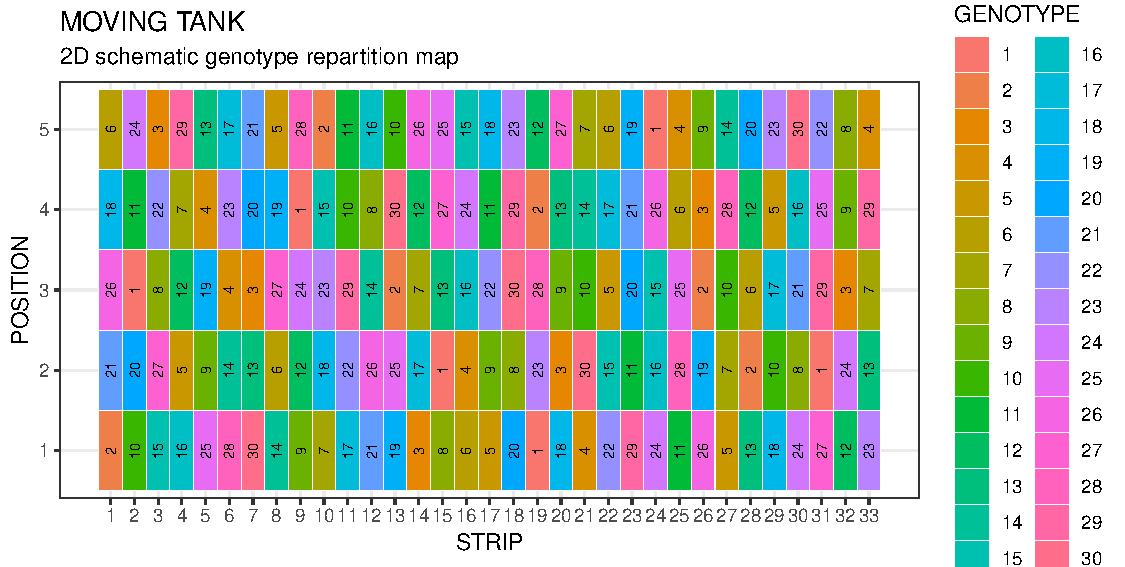
\includegraphics[width=\textwidth]{../../Figures/design_layout_moving.pdf} 
    \caption{2D schematic representation of the experimental design for 33 individual strips and 30 genotypes in the moving 
    tank.}
    \label{fig:moving_layout_30_geno}
\end{sidewaysfigure}

\begin{sidewaysfigure}[ht]
    \includegraphics[width=\textwidth]{../../Figures/design_layout_still.pdf} 
    \caption{2D schematic representation of the experimental design for 33 individual strips and 30 genotypes in the still 
    tank.}
    \label{fig:still_layout_30_geno}
\end{sidewaysfigure}

\subsection{Design's characteristics}


\section{Phenotyping experiment}
The phenotyping experiment took place between February 25th and March 13th. The seeds were first germinated and then transferred 
onto the platform. After the end of the experiment the plants were weighted, dried and weighted again to obtain dry and fresh 
weight.

\subsection{Germination}
Previous experiments in the greenhouses showed that germination of maize seeds on the platform often lead to asphyxiation of the 
seeds. 
Because of this, the seeds were germinated in an outside germination chamber and were only transferred onto the platform once 
germinated.

The seeds were placed in a temperature-controlled room at 20$^{\circ}$C for 3 days, inside a germination chamber. The chamber consisted of 2 PVC trays to which an air-fog machine was connected, to keep the seeds moist. 
Inside each tray, PVC plates were disposed diagonally and evenly spaced (fig. \ref{fig:germination_chamber_diagram}). On those plates, the seeds were arranged on a filtering paper sheet with ledges to support the weight of the seeds (figure \ref{fig:germiantion_ledge} and figure \ref{fig:photo_germination_plate}). The bottom of the trays were filled with water to keep the filtering paper moist. 
There were 17 plates in total, 15 for the 30 genotypes and 2 for the border genotype (150 seeds dispatched on 2 plates). 

    \begin{figure}[!htb]
        \centering
        \begin{subfigure}[b]{0.95\textwidth}
            \centering
            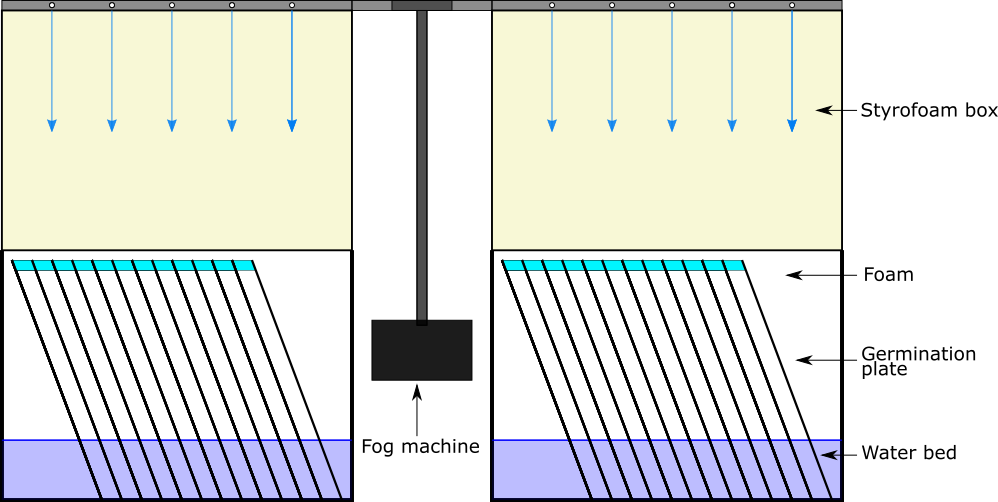
\includegraphics[width=\textwidth]{figures/germination_chamber_diagram.png}
            \caption[]%
            {Global schematic view of the germination chamber: a fog machine assure constant humidity in the germination 
            chambers by creating fog at regular intervals (the blue arrows represent the path of the fog). The plates are placed 
            at a 60$^{\circ}$ angle and 5 cm apart}    
            \label{fig:germination_chamber_diagram}
        \end{subfigure}
        \vskip\baselineskip
        \begin{subfigure}[b]{0.475\textwidth}   
            \centering 
            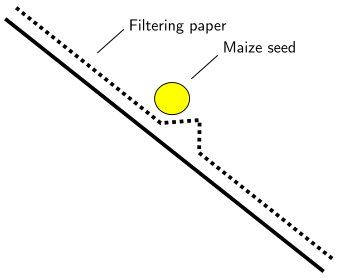
\includegraphics[width=\textwidth]{figures/germination_ledge.png}
            \caption[]%
            {Schematic view of a germination ledge on a PVC plate: each seed is fixed in position on the ledge by an additional 
            drop of agar solution to avoid any fall-off}    
            \label{fig:germiantion_ledge}
        \end{subfigure}
        \quad
        \begin{subfigure}[b]{0.475\textwidth}   
            \centering 
            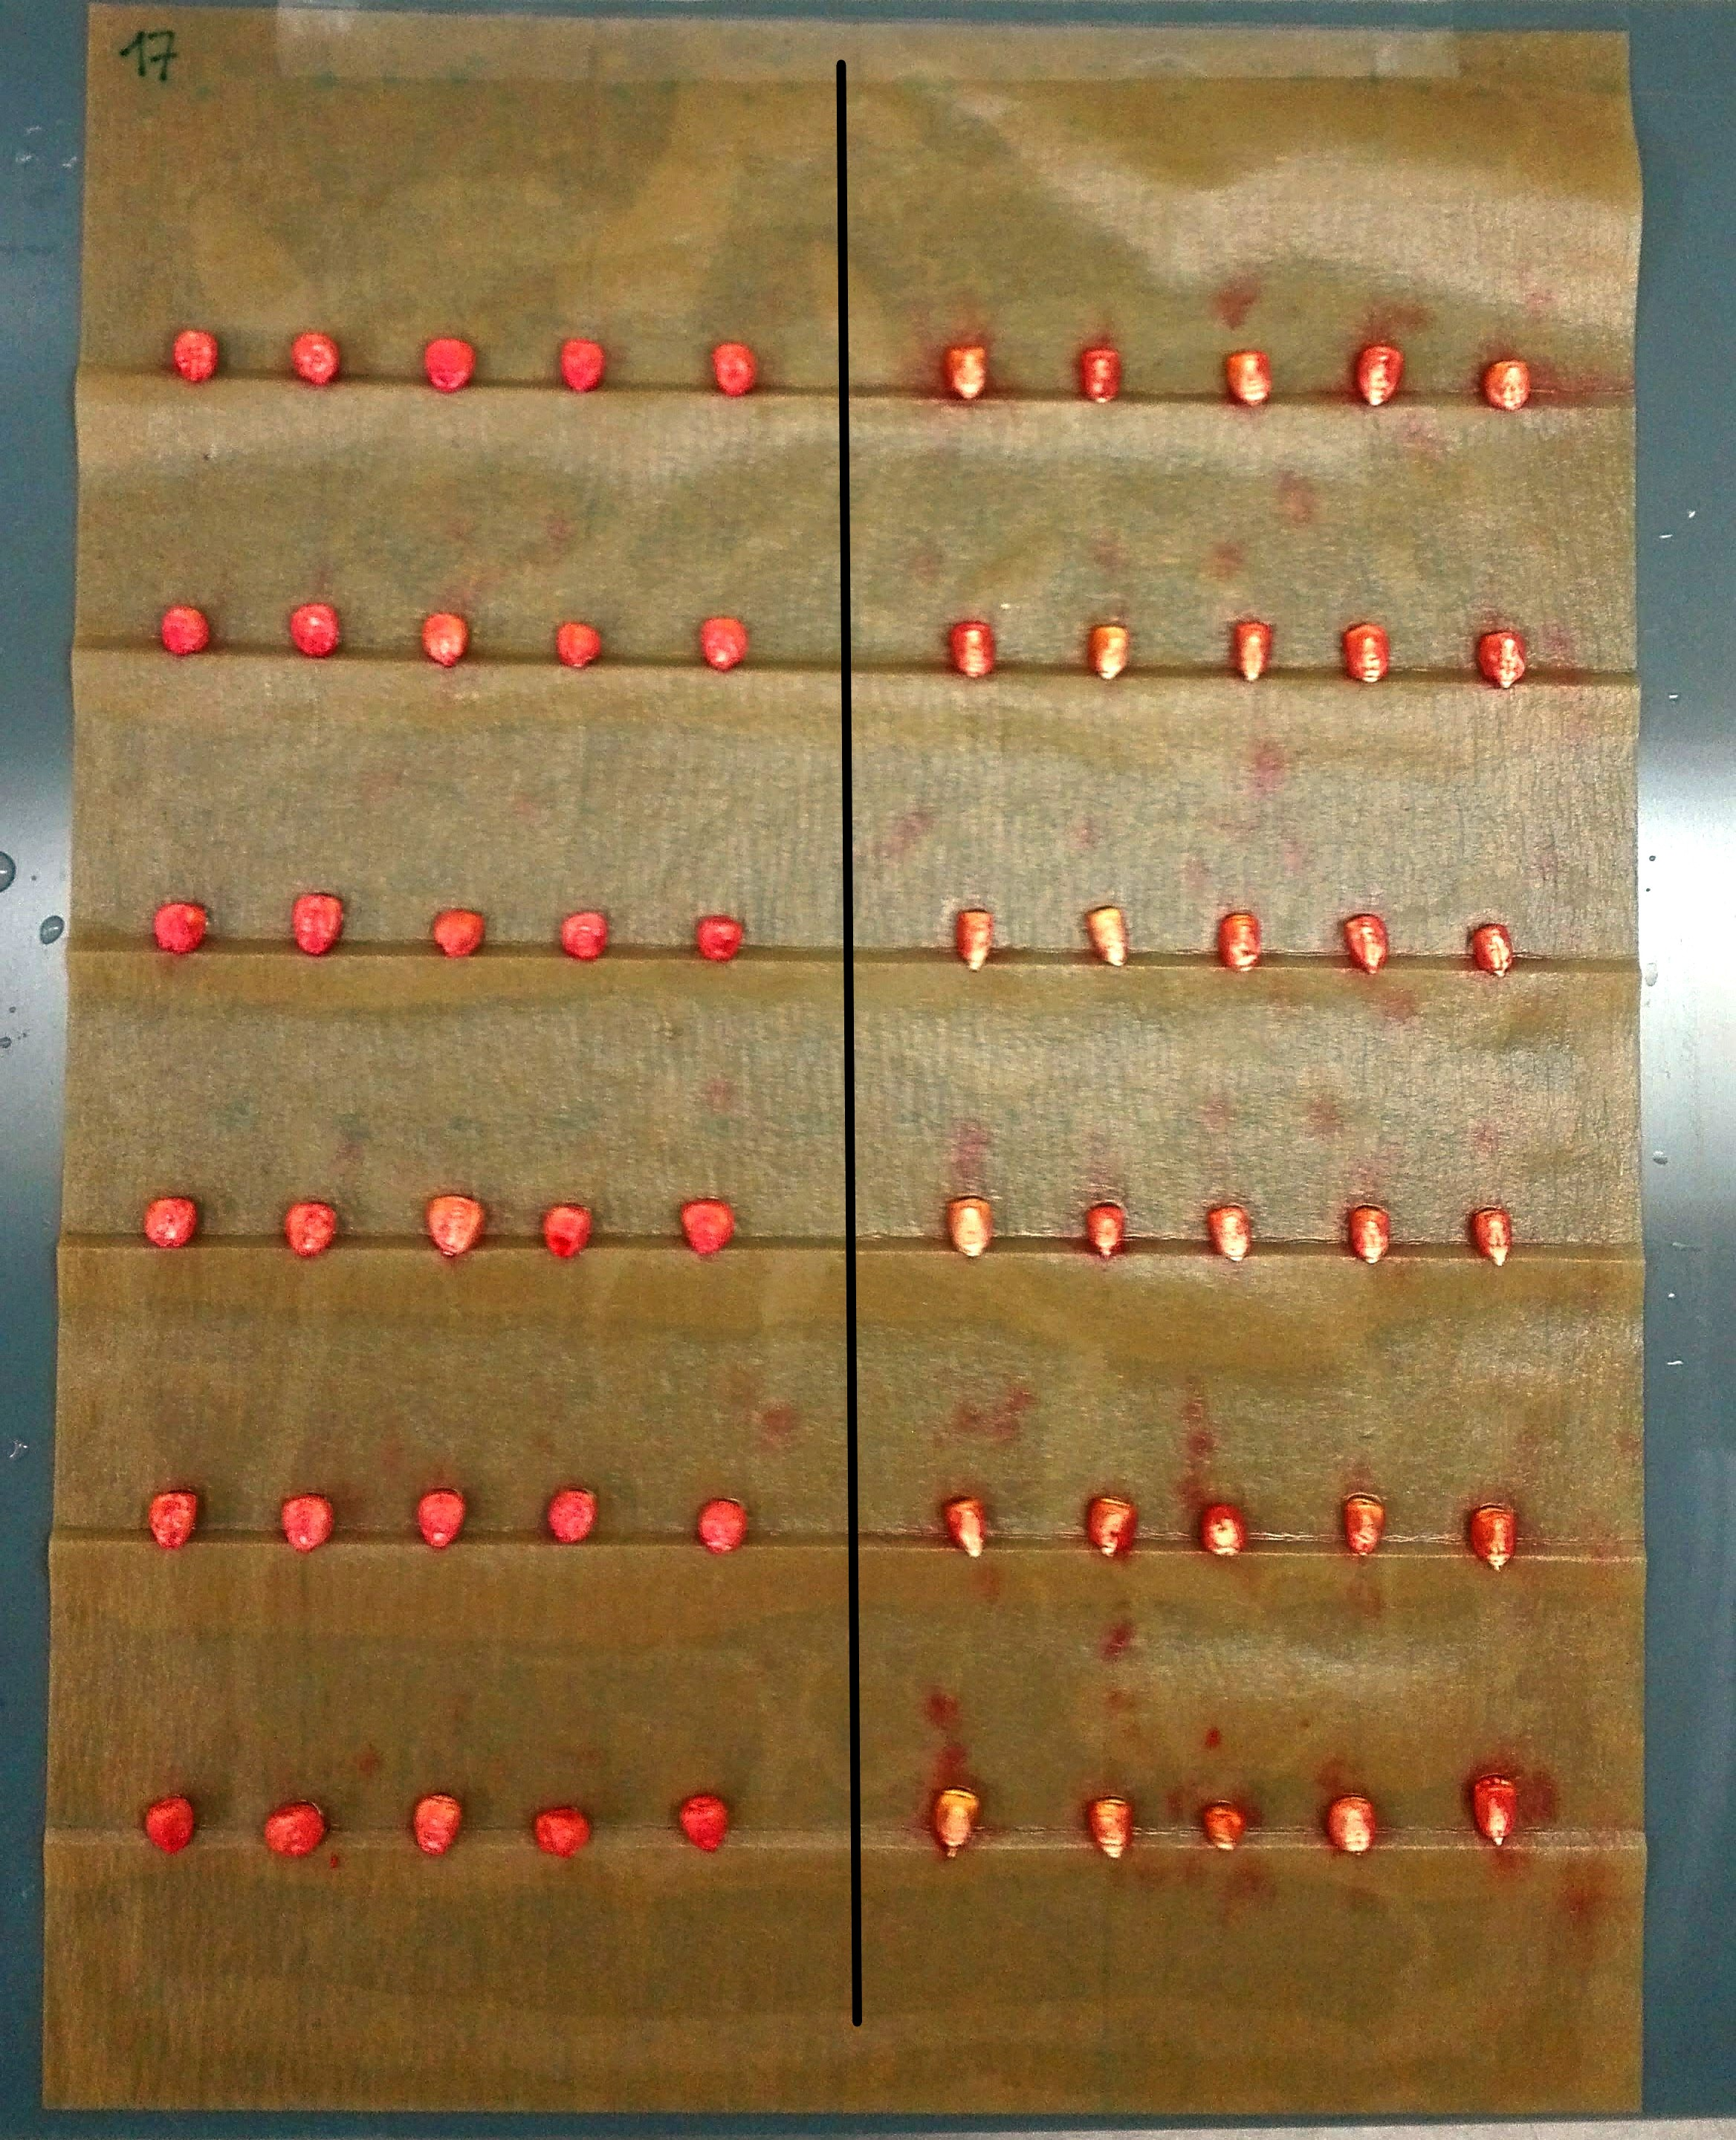
\includegraphics[width=\textwidth]{figures/photo_germination_plate.jpg}
            \caption[]%
            {30 cm by 40 cm PVC plate with seeds on filtering paper (the black line represents the separation between the two 
           genotypes on the plate). Each sheet had 6 rows of 10 seeds with one genotype on the left and one genotype on the 
           right.}    
            \label{fig:photo_germination_plate}
        \end{subfigure}
        \caption{Germination chamber diagram with detailed view and pictures}
    \end{figure}

After 3 days into the chamber, not all seeds were germinated, table \ref{tab:germination_percentage} presents the germination 
rates and mean seed weights for all the genotypes used (including the border genotype). The non-germination was mainly due to 
the fact that seeds fell into the water bed and because mold grew on some filtering paper.

%table for the germination rates after the outside germination process

\begin{table}[ht]
\centering
\caption[Germination rates and seed weights]{Germination rate and mean seed weight for each genotype used. (there is no data concerning the germination rate of the 
border genotype because it was not measured).}

\rowcolors{2}{gray!25}{white}

\begin{tabular}{lcc}
  \toprule
  %\rowcolor{gray!50}
Genotype & Germination rate (\%) & Mean seed weight (g) \\ 
  \midrule
1 & 80.00 & 0.28 \\ 
  2 & 86.67 & 0.36 \\ 
  3 & 96.67 & 0.36 \\ 
  4 & 73.33 & 0.28 \\ 
  5 & 100.00 & 0.32 \\ 
  6 & 96.67 & 0.24 \\ 
  7 & 96.67 & 0.19 \\ 
  8 & 70.00 & 0.31 \\ 
  9 & 96.67 & 0.33 \\ 
  10 & 96.67 & 0.25 \\ 
  11 & 60.00 & 0.33 \\ 
  12 & 93.33 & 0.27 \\ 
  13 & 90.00 & 0.24 \\ 
  14 & 86.67 & 0.31 \\ 
  15 & 56.67 & 0.35 \\ 
  16 & 90.00 & 0.28 \\ 
  17 & 90.00 & 0.30 \\ 
  18 & 86.67 & 0.26 \\ 
  19 & 100.00 & 0.26 \\ 
  20 & 86.67 & 0.28 \\ 
  21 & 86.67 & 0.32 \\ 
  22 & 53.33 & 0.30 \\ 
  23 & 73.33 & 0.28 \\ 
  24 & 100.00 & 0.16 \\ 
  25 & 96.67 & 0.19 \\ 
  26 & 96.67 & 0.25 \\ 
  27 & 96.67 & 0.28 \\ 
  28 & 83.33 & 0.36 \\ 
  29 & 93.33 & 0.30 \\ 
  30 & 73.33 & 0.35 \\ 
  31 & / & 0.38 \\ 
   \bottomrule
\end{tabular}
\label{tab:germination_percentage}
\end{table}

\subsection{Phenotyping platform}
The phenotyping platform is located inside a greenhouse in the facilities of the UCLouvain (Louvain-la-Neuve, Belgium). 
It consists of two aeroponic tanks on which are arranged 99 styrofoam strips, each with five holes. 
At the end of each tank is a high definition camera that scans the root system of each plant individually, when it passes in 
front of it (fig. \ref{fig:tank}). 
The strips rotate in a clockwise fashion in the tank and a full rotation is completed in 2 hours. 
Three sprinklers are placed regularly at the bottom of each side of the tank (fig. \ref{fig:tank_transversal_view}). 
The sprinklers spray nutrient solution\footnote{The precise concentration of the Hoagland solution is presented in appendix 
\ref{appendix:hoagland}} at regular intervals, set by the operator. 
The spraying pattern (interval and duration) can be differentiated between day and night and can be modified at any moment of 
the experiment.
In this case the patterns were 5 seconds of spraying ever 295 seconds all the time.
During the experiment, the temperature of the greenhouse was set to 20$^{\circ}$C at day and 18$^{\circ}$C at night and the 
lights were on from 6 AM to 10 PM. 
At the start of the experiment seeds were placed inside a foam cork and then placed inside a hole on a strip (fig 
\ref{fig:seed_platform_close_up}). 
They were placed at the bottom to allow the root system to grow freely. 
The corks are drilled vertically to let the leaf system develop with less resistance and allow a direct access to sunlight. 
More information about the platform is available in appendix \ref{appendix:platform_info}.

After 3 days in the germination chamber, the germinated seeds were transferred onto the platform following the created design, and the non-germinated seeds were discarded. The first tank was constantly moving but only scanning the root systems once a day, while the second tank was only moving once a day to scan the root system of the plants and stayed still the rest of the day.

\begin{figure}[!htb]
        \centering
        \begin{subfigure}[b]{0.95\textwidth}
            \centering
            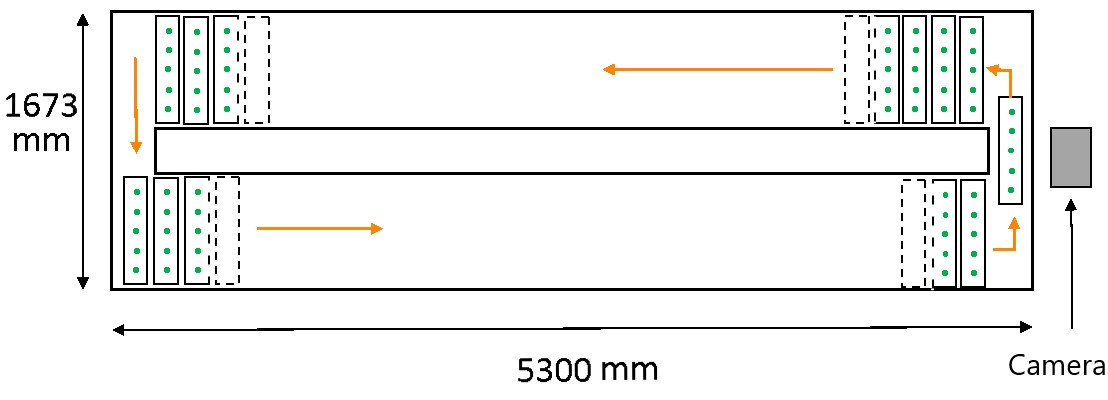
\includegraphics[width=\textwidth]{figures/tank.jpg}
            \caption{Schematic view of an aeroponic tank: plants are hold on strips, 5 plants per strip (green dots on layout). There are 99 strips in the tank for a total of 495 plants/tank. Strips move in the direction indicated by orange arrows}    
            \label{fig:tank}
        \end{subfigure}
        \vskip\baselineskip
        \begin{subfigure}[b]{0.475\textwidth}   
            \centering
            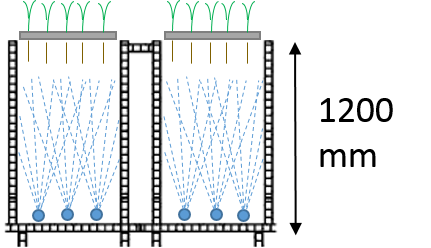
\includegraphics[width=\textwidth]{figures/tank_transversal_view.png}
            \caption{Transversal schematic view of an aeroponic tank of the platform: at the bottom of each tank, sprinklers (represented in blue in the layout) are disposed at regular interval and spray nutritive solution}    
            \label{fig:tank_transversal_view}
        \end{subfigure}
        \quad
        \begin{subfigure}[b]{0.475\textwidth}   
            \centering
            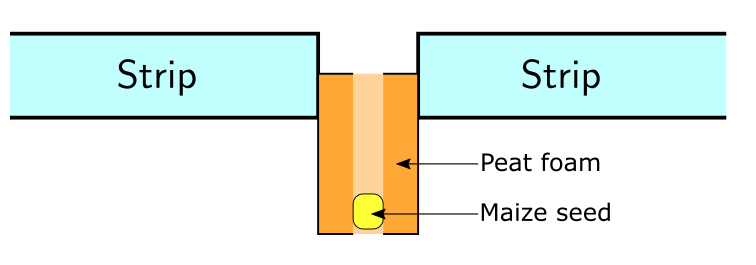
\includegraphics[width=\textwidth]{figures/seed_platform_close_up.png}
            \caption{Close up schematic view of a strip: inside each hole, seeds are placed inside a pierced peatfom cork to allow the root system to develop frelly}    
            \label{fig:seed_platform_close_up}
        \end{subfigure}
        \caption{Detailed diagrams about the phenotyping platform}
    \end{figure}


\section{Data processing}
After 15 days, the plants were considered fully grown and the experiment was stopped. The leaf and root systems were separated and weighted individually on scales precise to 0.001 g. They were then dried for 3 days in a 70$^{\circ}$C oven. After the drying process, they were weighted again. For each plant, the remaining of the seed was consistently kept on the root system.
Two kind of data were obtained from the experiment: weight data (dry and fresh) of the fully grown plants and root scan data. Five variables were kept for the spatial analysis:

\begin{itemize}
\item $FRESH\_RS$: fresh weight of the root system
\item $FRESH\_LS$: fresh weight of the leaf system
\item $DRY\_RS$: dry weight of the root system
\item $DRY\_LS$: dry weight of the leaf system
\item $AREA$: percentage of the total area occupied by the root system
\end{itemize} 

To be used as inputs in the models, those data need to be processed. The following sections details this step.

\subsection{Weight data}
For some plants, the germinated seeds placed on the platform did not fully grow or had an abnormal growth, but all the plants were still weighted to avoid leaving out any data. Therefore some data points need to be handled more carefully, as they do not represent the genotype's growth correctly. However, a correct growth, representative of the genotype, is hard to define because the influence of the conditions on each genotype is unknown. Therefore, instead of choosing which plants are outliers in a binary way, we attributed weights to each plant to express the quality of the data. Those weights were established by reviewing the final root scan of each plant and checking the different factors that could have an influence. The factors chosen are the following:

\begin{itemize}
\item $NO\_RS$: no additional root to the primary root
\item $NO\_LS$: no visible leaf system 
\item $BAD\_LS$: leaf system grew under the strip (or abnormally in general)
\item  $NO\_SEED$: no seed (or an empty cork) present on this position
\item $NOT\_FG$: plant not fully grown
\item $OVERLAP$: leaf (or root) system of another plant overlaps on the root scan
\item $OK$: no influential factors
\end{itemize} 

An visualization of those factors with example pictures is presented in figure \ref{fig:example_influential_factors}. Some plants were attributed several influential factors, but $OK$, $NO\_SEED$ and $NOT\_FG$ were considered as exclusive. The factor attribution was ambiguous for some pictures, in those cases the plant were considered $OK$ to avoid losing any data points.
Following the determination of the factors, weights were attributed to each variable according to the weight matrix, presented in table \ref{tab:weight_attribution_matrix}.


% Table generated by Excel2LaTeX from sheet 'weights'
\begin{table}[htbp]
  \centering
  \caption[Weight attribution matrix]{Weight attribution matrix for the different factors and variables. LS weight is both the fresh and dry weight for leaf system and RS weight is the same for the root system}
  	\rowcolors{2}{gray!25}{white}
    \begin{tabular}{lrrr}
    \toprule
    CODE  & LS weight & RS weight & Area \\
    \midrule
    NO\_RS & 1     & 1     & 1 \\
    NO\_LS & 2     & 2     & 2 \\
    BAD\_LS & 3     & 3     & 3 \\
    NOT\_FG & 4     & 4     & 4 \\
    NO\_SEED & 0	& 0		& 0 \\
    OK 		& 5 	& 5 	& 5 \\
    OVERLAP & 5     & 5     & 0 \\
    \bottomrule
    \end{tabular}%
  \label{tab:weight_attribution_matrix}%
\end{table}%


\begin{sidewaysfigure}[ht]
\centering
\begin{subfigure}[t]{.13\textwidth}
  \centering
  \includegraphics[width=\linewidth]{figures/NO_RS.jpg}
  \caption{$NO_RS$: no additional root, other than the primary}
  \label{fig:NO_RS}
\end{subfigure}
%
\begin{subfigure}[t]{.13\textwidth}
  \centering
  \includegraphics[width=\linewidth]{figures/NO_LS.jpg}
  \caption{$NO\_LS$: no apparent leaf system}
  \label{fig:NO_LS}
\end{subfigure}
%
\begin{subfigure}[t]{.13\textwidth}
  \centering
  \includegraphics[width=\linewidth]{figures/BAD_LS.jpg}
  \caption{$BAD\_LS$: the leaf system grew under the strip and deviated to the right (obstruction of another plant)}
  \label{fig:BAD_LS}
\end{subfigure}
%
\begin{subfigure}[t]{.13\textwidth}
  \centering
  \includegraphics[width=\linewidth]{figures/NO_SEED.jpg}
  \caption{$NO\_SEED$}
  \label{fig:NO_SEED}
\end{subfigure}
%
\begin{subfigure}[t]{.13\textwidth}
  \centering
  \includegraphics[width=\linewidth]{figures/NOT_FG.jpg}
  \caption{$NOT\_FG$: both system are present but underdeveloped compared to other images }
  \label{fig:NOT_FG}
\end{subfigure}
%
\begin{subfigure}[t]{.13\textwidth}
  \centering
  \includegraphics[width=\linewidth]{figures/OVERLAP.jpg}
  \caption{$OVERLAP$: the leaf system of another plant hides the root system of the plant}
  \label{fig:OVERLAP}
\end{subfigure}
%
\begin{subfigure}[t]{.13\textwidth}
  \centering
  \includegraphics[width=\linewidth]{figures/OK.jpg}
  \caption{$OK$, the green box represents the bounding area for the computation of the root area}
  \label{fig:OK}
\end{subfigure}
%
\caption{Example pictures of the influential factors chosen for the weight attribution.}
\label{fig:example_influential_factors}
\end{sidewaysfigure}

\subsection{Root pictures}
The area of the root system was computed using the final root scan of each plant. Each picture was converted to gray-scale, resized to a specific bounding rectangle and binarized. The bounding box is illustrated on figure \ref{fig:OK}. The threshold for the binarization was 140 on a 0 to 255 scale. Since the roots are black on the original picture, the binarization was completed without any issues. The area of the root system was expressed as a percentage of the total area of the bounding box, by counting the black pixels in the image. All the processing was done in python using the opencv package.


\section{SpATS model}
In this section, the SpATS model is introduced. For a more thorough treatment of the model and all its components, see \textcite{rodriguez-alvarez_spatial_2016}.\\
Consider a field trial of $n$ plots arranged in a rectangular grid, where the plot positions are collected in vectors of row $(\mathbf{r})$ and column $(\mathbf{c})$ coordinates. If $\mathbf{y}$ is the vector of plot data in field order, a common model for $\mathbf{y}$, to use as a starting point is
	\begin{equation}
	    \boldsymbol{y}=\mathbf{1}_{n} \beta_{0}+\boldsymbol{Z}_{r} \boldsymbol{c}_{r}+\boldsymbol{Z}_{c} \boldsymbol{c}_{c}
	    +\varepsilon
	\end{equation}
were $\mathbf{1}_{n}$ is a column-vector of ones of length $n$, $\boldsymbol{c}_{r}$ and $\boldsymbol{c}_{c}$ are, respectively, the random effect coefficients for the rows and columns and associated matrix $\boldsymbol{Z}_{r}$ and $\boldsymbol{Z}_{c}$. To fully capture complex spatial patterns, a smooth bivariate surface jointly defined over the row and column positions is added to the model, which becomes
	\begin{equation}
	    \boldsymbol{y}=f(\boldsymbol{u}, \boldsymbol{v})+\boldsymbol{Z}_{r} \boldsymbol{c}_{r}+\boldsymbol{Z}_{c} \boldsymbol{c}
	    _{c}+\boldsymbol{\varepsilon}
	    \label{eq:base_model_bismooth_surface}
	\end{equation}
where $\mathbf{u}$ and $\mathbf{v}$ are, respectively, the vector of row and columns positions and where $f(.,.)$ represents the smooth bivariate function. Note that the intercept term, $\beta_0$ is embedded into $f(u,v)$. To better understand this function, let us decompose it in a nested-ANOVA structure
	\begin{align}
	f ( \boldsymbol { u } , \boldsymbol { v } ) & = \underbrace { \mathbf { 1 } _ { n } \beta _ { 0 } + \boldsymbol { u } \beta
	 _ { 1 } + \boldsymbol { v } \beta _ { 2 } + \boldsymbol { u } \odot \boldsymbol { v } \beta _ { 3 } } _ { \text { Bilinear
	  polynomial } } \nonumber \\
	 & + \underbrace { f _ { u } ( \boldsymbol { u } ) + f _ { v } ( \boldsymbol { v } ) + \boldsymbol { u } \odot h _ { v } (
	  \boldsymbol { v } ) + \boldsymbol { v } \odot h _ { u } ( \boldsymbol { u } ) + f _ { u , v } ( \boldsymbol { u } ,
	   \boldsymbol { v } ) }_{\text{Smooth part}}
	 \label{eq:full_bivariate_smooth_surface_model}
	\end{align}
where $\odot$ denotes the element-wise matrix product\footnote{See appendix \ref{appendix:add_info} for details about the element-wise matrix product.}. There are now two components to the model: a bilinear polynomial part(parametric) and a smooth part (non-parametric). The parametric part includes the linear trends along rows ($\beta_1$) and columns ($\beta_2$) as well as a linear interaction trend ($\beta_3$). The smooth part models the deviation from the compound linear trend, and can be decomposed in the following elements:
	\begin{itemize}
		\item $f_{u}(\boldsymbol{u})$  is a smooth trend along the rows, identical for all columns (i.e., a main smooth effect).
		\item $f_{v}(\boldsymbol{v})$ is a smooth trend along the columns, identical for all rows.
		\item $\boldsymbol{v} \odot h_{u} (\boldsymbol{u})$ and $\boldsymbol{u} \odot h_{v} (\boldsymbol{v})$ are linear-by-
		smooth interaction trends. For instance, $\boldsymbol{u} \odot h_{v}(\boldsymbol{v})$ is a varying coefficient surface 
		trend, consisting of functions, linear in the rows, for each column, but with slopes that change smoothly along the 
		columns, $h_{v}boldsymbol{v})$.
		\item $f_{u,v}(\boldsymbol{u},\boldsymbol{v})$ is a smooth-by-smooth interaction trend jointly defined over the row and 
		column directions.
	\end{itemize}
In total, six components are used to model the surface $f$. This may seem like a lot but this allows the translation of model \ref{eq:base_model_bismooth_surface} into a standard mixed model. An interesting property of this proposal is that since $u$ and $v$ are row and column position, it allows depicting the spatial trend in a grid finer than the number of rows and columns. Figure \ref{fig:bilinear_and_smooth_decomposition} shows an example of those six components in the context of a barley uniformity performed by \textcite{williams1988contemporary}. It shows clearly how the additional components, help to capture small variations in the spatial data.

\begin{figure}[hbtp]
\centering
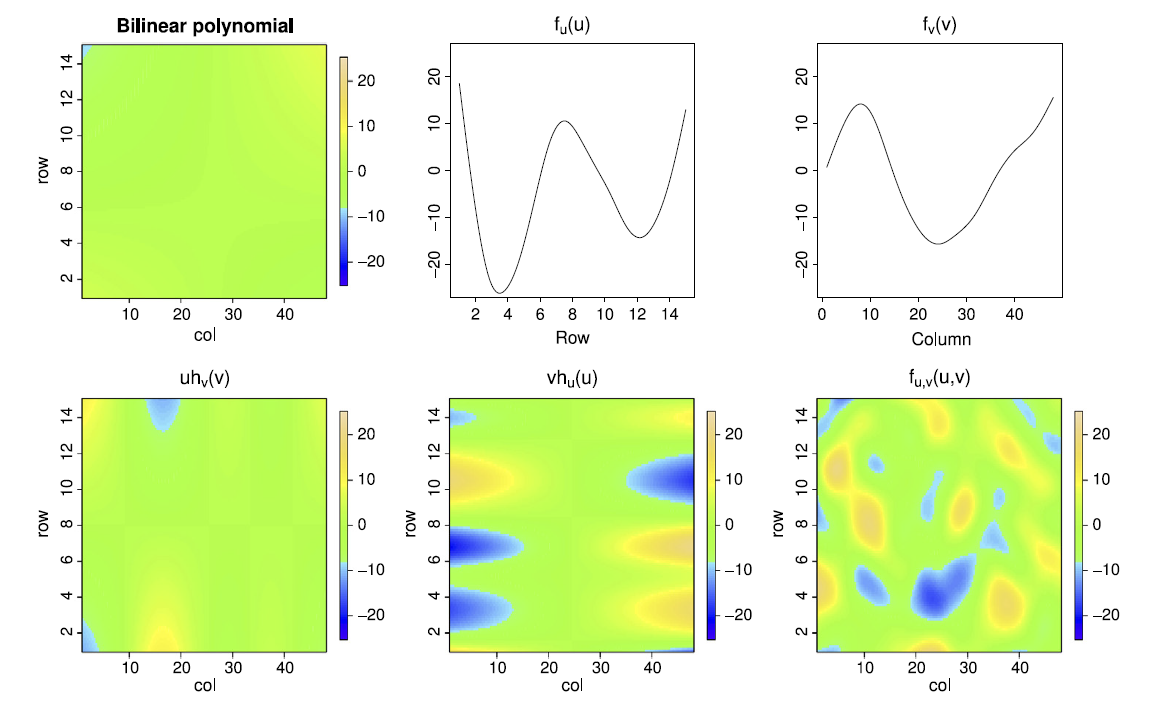
\includegraphics[width=\textwidth]{../figures/bilinear_polynomial.PNG}
\caption[Bilinear and smooth components of the PS-ANOVA decomposition]{Bilinear and smooth components of the PS-ANOVA decomposition of the estimated spatial trend for the barley uniformity
data from \textcite{rodriguez-alvarez_correcting_2018}.}
\label{fig:bilinear_and_smooth_decomposition}
\end{figure}


\subsection{Modelling using P-splines}
The functions $f_u$, $f_v$, $h_u$ and $h_v$ are constructed  with variations on one-dimensional P-splines, while $f_{u,v}$ is based on tensor products P-splines.\\
For clarity's sake, let us consider a model only containing a smooth bivariate surface and an error term
	\begin{equation}
	    y _ { i } = f \left( u _ { i } , v _ { i } \right) + \varepsilon _ { i } , \text { with } \varepsilon _ { i } \sim N 
	    \left( 0 , \sigma ^ { 2 } \right) \text{.}
		\label{eq:smooth_part_only_model}
	\end{equation}
\textcite{lee_efficient_2013} show that it can be represented using B-splines\footnote{See appendix \ref{appendix:add_info} for details about B-splines and P-splines.}. Let us form two B-splines basis:
\begin{enumerate}
\item one for the columns, $\boldsymbol{\invbreve{B}}$ with $ b_{il}= \invbreve{B}_l(u_i)$, where $\invbreve{B}_l(u_i)$ is the $l$th B-spline of the basis, evaluated at $u_i$
\item and one for the rows, $\boldsymbol{\breve{B}}$ with $ b_{ip}= \breve{B}_p(v_i)$, where $\breve{B}_l(v_i)$ is the $p$th B-spline of the basis, evaluated at $v_i$.
\end{enumerate}
Then, the smooth-by-smooth interaction can be written using those basis
\begin{equation}
	f \left(u_{i},v_{i}\right)=\sum_{l=1}^{L}\sum_{p=1}^{P}\invbreve{B}_{l}\left(u_{i}\right)\breve{B}_{p}\left(v_{i}\right) 
	\alpha_{lp}\text{,}
\end{equation}
where $\boldsymbol{\alpha} = (\alpha_{11},\ldots,\alpha_{1P},\ldots,\alpha_{LP})^t$ is a vector of unknown regression coefficients of dimension $(LP \times 1)$. Note that $\boldsymbol{\invbreve{B}}$ and $\boldsymbol{\breve{B}}$ are matrices of order $n \times L$ and $n\times P$ respectively, where $L$ and $P$ are the number of the B-spline basis functions. \textcite{dierckx_curve_1995} shows that, in the P-spline framework, the smooth-by-smooth interaction $f(u_i,v_i)$ is modelled by the tensor product of B-splines bases. Then, we can write, in matrix notation,
\begin{equation}
    \boldsymbol{B} = \boldsymbol{\invbreve{B}} \boxdot \boldsymbol{\breve{B}} = \left( \boldsymbol{\invbreve{B}} \otimes
    \boldsymbol{1} _ { L } ^ { t } \right) \odot \left( \mathbf { 1 } _ { P } ^ { t } \otimes \boldsymbol{\breve{B}} \right)
    \text{,}
\end{equation}
where the operation $\boxdot$ is defined in terms of the Kronecker product of two matrices (denoted by $\otimes$) and the 
element-by-element multiplication of two matrices (denoted by $\odot$)\footnote{See appendix \ref{appendix:add_info} for details 
about the Kronecker, and the element-wise products}. Therefore model (\ref{eq:smooth_part_only_model}) can be written in matrix 
notation:

\begin{equation}
    \boldsymbol{y} = \boldsymbol{B}\boldsymbol{\alpha} + \boldsymbol{\epsilon}
    \text{.}
    \label{eq:spline_model_mat_form}
\end{equation}

The coefficients of this parametric model can be estimated by minimizing the sum of squares. The explicit solution is then:
\begin{equation}
	\Hat{\boldsymbol{\alpha}} = (\mathbf{B}^t\mathbf{B})^{-1}\mathbf{B}^t\mathbf{y}
\end{equation}
To prevent over-fitting, 
\textcite{eilers_flexible_1996} propose to incorporate a discrete penalty on the coefficient associated to adjacent B-splines.
As described in details in appendix \ref{appendix:polynomial_splines}, this penalty also determines the smoothness of the 
splines. The solution of equation \ref{eq:spline_model_mat_form} then becomes 
\begin{equation}
    \widehat{\boldsymbol{\alpha}}=\left(\boldsymbol{B}^{t} \boldsymbol{B}+\boldsymbol{P}\right)^{-1} \boldsymbol{B}^{t} 
    \boldsymbol{y}
    \text{,}
\end{equation}
where $\boldsymbol{P}$ is the penalty matrix. The details of this solution are presented in appendix 
\ref{appendix:penalized_solution_form}, but the important point to remember here, is that the smoothness of the bivariate 
surface is defined by the penalty matrix, which only depend on two tuning parameters  $\invbreve{\lambda}$ (smoothing along the 
columns) and $\breve{\lambda}$ (smoothing along the rows).

\subsection{Mixed model based smoothing parameter selection}

As explained in \textcite{rodriguez-alvarez_spatial_2016}, $\mathbf{P}$ is rank-deficient, meaning that the rank is smaller than the 
number of rows and/or columns, and this causes numerical instability when applying mixed model estimation techniques. To obtain 
a full-rank penalty matrix, the key is to write model \ref{eq:spline_model_mat_form} as 
\begin{equation}
    \mathbf{B}\boldsymbol{\alpha} = \boldsymbol{X}_{s} \boldsymbol{\beta}_{s}+\boldsymbol{Z}_{s} \boldsymbol{c}_{s}
    \text{.}
\end{equation}
There are now two bases: $\mathbf{X}_{s}$, with coefficients that are not penalized at all, and $\mathbf{Z}_{s}$, with a size 
penalty on its coefficients. This decomposition follows the proposal by \textcite{lee_p-spline_2011}, based on eigenvalue 
decomposition which gives rise to a diagonal penalty matrix.\\
The two bases have the following structures:
\begin{equation}
    \boldsymbol{X}_{s}=\left[\mathbf{1}_{n}, \boldsymbol{u}, \boldsymbol{v}, \boldsymbol{u} \odot \boldsymbol{v}\right]
    \quad
    \text{and}
    \quad
    \mathbf{Z}_{s}=\left[\mathbf{Z}_{v}, \mathbf{Z}_{u}, \mathbf{Z}_{v} \square \mathbf{u}, \mathbf{v} \square \mathbf{Z}_{u}, 
    \mathbf{Z}_{v} \square \mathbf{Z}_{u}\right]
    \text{,}
    \label{eq:detail_Xs_Zs_matrices}
\end{equation}
where $\boldsymbol{u}$ and $\boldsymbol{v}$ are still, respectively, the vectors of row and column positions. 
Here $\mathbf{Z}_{u}$ and $\mathbf{Z}_{v}$ are penalized version of the B-splines basis $\breve{\mathbf{B}}$ (rows) and
$\invbreve{\mathbf{B}}$ (columns). This new way of writing the problem leads to another penalty matrix 
$ \widetilde{\boldsymbol{P}}$, which is a block diagonal matrix. Each block of $ \widetilde{\boldsymbol{P}}$ corresponds to a 
block in $\mathbf{Z}_{s}$. Similarly to $\boldsymbol{P}$, the penalty matrix of the previous section, this new penalty matrix 
only depends on the two tuning parameters $\invbreve{\lambda}$ (smoothing along the columns) and $\breve{\lambda}$ (smoothing 
along the rows).
Figure \ref{fig:matrix_diagram} presents a diagram clarifying the structures and relations of the different matrices presented 
throughout this section.

This reformulation provides the ANOVA type decomposition discussed in the previous section 
(\ref{eq:full_bivariate_smooth_surface_model}), and explains how the bilinear smooth surface can be modelled using P-splines and 
tensor products of P-splines.
The block structure of $\mathbf{X}_s$ and $\mathbf{Z}_s$ implies
\begin{equation}
    \begin{aligned} 
        f(\boldsymbol{u}, \boldsymbol{v}) & =\boldsymbol{X}_{s} \boldsymbol{\beta}_{s}+Z_{s} \boldsymbol{c}_{s} \\ 
        								  & =\mathbf{1}_{n} \beta_{0}+\boldsymbol{u} \beta_{1}+\boldsymbol{v} \beta_{2}+
        								  \boldsymbol{u} \odot \boldsymbol{v} \beta_{3} \\
        								  & + \underbrace{f_{v}(\boldsymbol{v})}_{\boldsymbol{Z}_{v} \boldsymbol{c}_{s 1}}+
        								  \underbrace{f_{u}(\boldsymbol{u})}_{\boldsymbol{Z}_{u} \boldsymbol{c}_{s 2}} +
        								  \underbrace{\boldsymbol{u} \odot h_{v}(\boldsymbol{v})}_{\left[\boldsymbol{Z}_{v} 
        								  \square \boldsymbol{u}\right] \boldsymbol{c}_{s 3}}+\underbrace{\boldsymbol{v} \odot 
        								  h_{u}(\boldsymbol{u})}_{\left[\boldsymbol{v} \square \boldsymbol{Z}_{u}\right] 
        								  \boldsymbol{c}_{s 4}} +\underbrace{f_{u, v}(\boldsymbol{u}, \boldsymbol{v})}
        								  _{\left[\boldsymbol{Z}_{v} \square \boldsymbol{Z}_{u}\right] \boldsymbol{c}_{s 5}}
        								  \text{,}
    \end{aligned}
\end{equation}
where $\boldsymbol{c}_{sk} \ (k = 1,\ldots,5)$ contains the elements of $\boldsymbol{c}_s$ that correspond to the $k$th block of $\boldsymbol{Z}_s$, i.e. $\boldsymbol{c}_s = (\boldsymbol{c}_{s1}^t,\ldots,\boldsymbol{c}_{s5}^t)^t$. The details about the specific block component of $\boldsymbol{Z}_s$ and the computation of the new penalty matrix are available in the paper of \textcite{rodriguez-alvarez_correcting_2018} and the appendices therein.

Therefore, using this new notation, model \ref{eq:smooth_part_only_model} that only contains a smooth bivariate surface and an error term can be rewritten in the following way:

\begin{equation}
    \boldsymbol{y}=\boldsymbol{X}_{s} \boldsymbol{\beta}_{s}+\boldsymbol{Z}_{s} \boldsymbol{c}_{s}+\boldsymbol{\varepsilon}, 	
    \text { with } 
    \boldsymbol{\varepsilon} \sim N\left(\mathbf{0}, \sigma^{2} \boldsymbol{I}_{n}\right) 
    \text { and } 
    \boldsymbol{c}_{s} \sim N\left(\mathbf{0}, \boldsymbol{G}_{s}\right)
    \text{,}
\label{eq:smooth_surface_PS_ANOVA_rewritten}
\end{equation}
where $\boldsymbol{G}_{s} = \sigma^2\widetilde{\boldsymbol{P}}^{-1}$. It is straightforward to see that $\boldsymbol{G}_{s}$ 
also has a block diagonal structure, similar to that of $\widetilde{\boldsymbol{P}}$ (this structure is also represented on 
figure \ref{fig:matrix_diagram}). 
However, $\boldsymbol{G}_{s}$ depends on two different parameters, $\breve{\sigma}^2 =\sigma / \breve{\lambda}$ and $
\invbreve{\sigma}^2 =\sigma / \invbreve{\lambda}$, which are variances parameters. 
As shown in the diagram in figure \ref{fig:matrix_diagram}, the same variance parameters control the smoothness of the both the 
main effects and interactions terms. 
This prevents the use of standard mixed models software for estimation since $\mathbf{G}_s$ has its last block depending on both 
$\breve{\sigma}^2$ and $\invbreve{\sigma}^2$, but in a non-linear way. 
Even though \textcite{rodriguez-alvarez_fast_2015} presented a specialized algorithm to deal with this issue, 
here the PS-ANOVA decomposition approach \parencite{lee_efficient_2013} is used to allow the use of standard mixed model estimation procedures.\textcite{lee_efficient_2013} therefore propose to use a different variance component for each smooth component in $\mathbf{G}_s$, thus redefining this matrix as a linear function of variance parameters:
\begin{equation}
    \boldsymbol{G}_{s} = 
%	\bigoplus_{k=1}^{5} \sigma_{s k}^{2} \Lambda_{s k} =
    \bigoplus_{k=1}^{5} \boldsymbol{G}_{s k}= 
    \text{ blockdiag }
    \left(\boldsymbol{G}_{s 1}, \boldsymbol{G}_{s 2}, \boldsymbol{G}_{s 3}, \boldsymbol{G}_{s 4}, \boldsymbol{G}_{s 5}\right)
    \text{,}
\end{equation}
where $\boldsymbol{G}_{s k}$ %= \sigma_{sk}^2\boldsymbol{\Lambda}_{sk} \ (k=1,\ldots,5)$
is the $k$th block of the $\mathbf{G}_{s}$ matrix, depending on the specific variance component $\sigma_{sk}^2$. 
In other words, here the tensor product P-splines mixed model is represented as the sum of 5 sets of mutually independent Gaussian random components $\mathbf{c}_{sk}$, each depending on one variance $\sigma_{sk}^2 \ (k=1,\ldots,5)$.\\
Within this mixed model framework, the smoothing parameters, defined earlier as the ratio between the residual variance and the
corresponding variance effect $\lambda_{sk} = \sigma^2_{e} / \sigma^2_{sk}$, are determined by restricted maximum likelihood (REML). Therefore the smoothness of the spatial surface is tuned by five distinct parameters, applying anisotropic (direction-dependant) smoothing. This parametrization provides flexibility to account for both global and local variations in the field. Furthermore, the decomposition of $f(\mathbf{u},\mathbf{v})$ enables a more explicit interpretation of the main patterns of spatial variation \parencite{rodriguez-alvarez_correcting_2018}.


% Redefine the main unit
\newcommand{\myunit}{1 cm}

\begin{figure}
\centering
\resizebox{\columnwidth}{!}{%
\begin{tikzpicture}[>=latex]

% Matrix
\matrix (xs) [matrix of math nodes,%
             left delimiter  = (,%
             right delimiter = )] at (-0.5,5*\myunit)
{%
  1_n   \\
  \mathbf{u}    \\
  \mathbf{v}    \\
  \mathbf{u} \odot \mathbf{v} \\
};
\node [draw,below=10pt] at (xs.south) 
    {$\mathbf{X}_{s}$};

% Matrix annotations
\node [anchor=west] at (0.5,5.8) {\textit{Intercept}};
\node [anchor=west] at (0.5,5.3) {\textit{Cols}};
\node [anchor=west] at (0.5,4.8) {\textit{Rows}};
\node [anchor=west] at (0.5,4.3) {\textit{Cols $\times$ Rows}};


% Matrix
\matrix (bs) [matrix of math nodes,%
             left delimiter  = (,%
             right delimiter = )] at (4.5*\myunit,5*\myunit)
{%
  \beta_{1} \\
  \beta_{2} \\
  \beta_{3} \\
  \beta_{4} \\
};
\node [draw,below=10pt] at (bs.south) 
    {$\boldsymbol{\beta}_{s}$}; 


% Matrix
\matrix (zs) [matrix of math nodes,%
             left delimiter  = (,%
             right delimiter = )] at (7*\myunit,5*\myunit)
{%
  Z_{v} \\
  Z_{u} \\
  \mathbf{u} \boxdot Z_{v} \\
  \mathbf{v} \boxdot Z_{u} \\
  Z_{u} \boxdot Z_{v} \\
};
\node [draw,below=10pt] at (zs.south) 
    {$\mathbf{Z}_{s}$};

% Matrix annotation
\node [anchor=west] at (8.2,6.2) {\textit{Smooth cols trend}};
\node [anchor=west] at (8.2,5.6) {\textit{Smooth rows trend}};
\node [anchor=west] at (8.2,5) {\textit{Linear-by-smooth cols trend}};
\node [anchor=west] at (8.2,4.4) {\textit{Linear-by-smooth rows trend}};
\node [anchor=west] at (8.2,3.8) {\textit{Smooth-by-smooth trend}};

% Matrix
\matrix (cs) [matrix of math nodes,%
             left delimiter  = (,%
             right delimiter = )] at (15*\myunit,5*\myunit)
{%
  \mathbf{c}_{s1} \\
  \mathbf{c}_{s2} \\
  \mathbf{c}_{s3} \\
  \mathbf{c}_{s4} \\
  \mathbf{c}_{s5} \\
};
\node [draw,below=10pt] at (cs.south) 
    {$\mathbf{c}_{s}$};

% matrix
\matrix (P) [matrix of math nodes,%
             left delimiter  = (,%
             right delimiter = )] at (0*\myunit,-1*\myunit)
{%
  \widetilde{\mathbf{P}}_{1} \propto \breve{\lambda} \\
  \widetilde{\mathbf{P}}_{2} \propto \invbreve{\lambda} \\
  \widetilde{\mathbf{P}}_{3} \propto \breve{\lambda} \\
  \widetilde{\mathbf{P}}_{4} \propto \invbreve{\lambda} \\
  \widetilde{\mathbf{P}}_{5} \propto \left(\breve{\lambda};
  \invbreve{\lambda}\right) \\
};
\node [draw,above=10pt] at (P.north) 
    {$\widetilde{\mathbf{P}}$};

% Matrix annotations
\node [below = 10pt, text width=3cm, align = center] at (P.south)
{Penalty term for each corresponding term in $\mathbf{Z}_{s}$};

% matrix
\matrix (gs) [matrix of math nodes,%
             left delimiter  = (,%
             right delimiter = )] at (7*\myunit,-1*\myunit)
{%
  \mathbf{G}_{s1} \propto \breve{\sigma}^{2} \\
  \mathbf{G}_{s2} \propto \invbreve{\sigma}^{2} \\
  \mathbf{G}_{s3} \propto \breve{\sigma}^{2} \\
  \mathbf{G}_{s4} \propto \invbreve{\sigma}^{2} \\
  \mathbf{G}_{s5} \propto \left(\breve{\sigma}^{2}; 
  \invbreve{\sigma}^{2}\right) \\
};
\node [draw,above=10pt] at (gs.north) 
    {$\mathbf{G}_{s}$};

% Matrix annotations
\node [below = 10pt, text width=4cm, align = center] at (gs.south){Variance terms for each corresponding term in $\mathbf{Z}_{s}$};

% Matrix
\matrix (gs2) [matrix of math nodes,%
             left delimiter  = (,%
             right delimiter = )] at (14*\myunit,-1*\myunit)
{%
  \mathbf{G}_{s1} \propto \breve{\sigma}^{2}_{s1} \\
  \mathbf{G}_{s2} \propto \invbreve{\sigma}^{2}_{s2} \\
  \mathbf{G}_{s3} \propto \breve{\sigma}^{2}_{s3} \\
  \mathbf{G}_{s4} \propto \invbreve{\sigma}^{2}_{s4} \\
  \mathbf{G}_{s5} \propto \left(\breve{\sigma}^{2}_{s5};
  \invbreve{\sigma}^{2}_{s5}\right) \\
};
\node [draw,above=10pt] at (gs2.north) 
    {$\mathbf{G}_{s} = \bigoplus_{k=1}^{5} \mathbf{G}_{sk}$};

% Matrix annotations
\node [below = 10pt, text width=4cm, align = center] at (gs2.south)
{Independent variance term for each corresponding term in $\mathbf{Z}_{s}$};

% Equation
\node at (7,9) {\large $\mathbf{y} = f(\mathbf{u},\mathbf{v}) + 
\boldsymbol{\epsilon} = \mathbf{B}\boldsymbol{\alpha} 
+\boldsymbol{\epsilon} = $};
\node at (6.15, 8.3) (XS) {\large $\mathbf{X}_{s}$};
\node  at (6.8, 8.3) (BS){\large $\boldsymbol{\beta}_{s}$};
\node at (7.2,8.3) (plus) {\large $+$};
\node at (7.65, 8.3) (ZS) {\large $\mathbf{Z}_{s}$};
\node at (8.05,8.3) (CS) {\large $\mathbf{c}_{s}$};
\node at (8.6,8.3) (epsilon) {\large $+ \boldsymbol{\epsilon}$};

% Arrows 
\draw [->] (XS.south) -- (xs.north);
\draw [->] (BS.south) -- (bs.north);
\draw [->] (ZS.south) -- (zs.north);
\draw [->] (CS.south) -- (cs.north);

% Relations
\draw [double, ->] ($(P.east) + (0.5,0)$) -- ($(gs.west) - (0.5,0)$) ;
\node [draw] at ($(P.east) + (2,0.5)$) {$\mathbf{G}_{s} = 
\sigma_{s}^{2}\widetilde{\mathbf{P}}^{-1}$};

\draw [double,->] ($(gs.east) + (0.5,0)$) -- ($(gs2.west) - (0.5,0)$);
\node [text width = 3cm, align = center, anchor = center] at ($(gs.east) + (1.8,1)$) {independent variance components};
%\node at (9,0.3) {components};
%\node at (9,0.7) {variance};
%\node at (9,1) {independent};

\end{tikzpicture}}
\caption[Diagram detailing the structure of the matrices used in this section]{Diagram detailing the structure of the matrices used in this section. All matrices are block diagonal matrix with each element represented on the diagram, being an individual block. The symbol $\propto$ shows how each block of the $\widetilde{\mathbf{P}}$/$\mathbf{G}_{s}$ matrix relates to the tuning/variance parameters.}
\label{fig:matrix_diagram}
\end{figure}


\subsection{Spatial models for field trials}
The tensor product P-spline, presented in the previous section, constitutes the base for the analysis of agricultural field trials because it allows the modeling of the random spatial variation typically presented in a field. 
On top of this spatial field, we need to build up a more complex models in order to account for the genetic variation, the different tanks, strips and positions. From now on, we therefore consider the following linear mixed model
\begin{equation}
    \boldsymbol{y}=
    \underbrace{
    	\boldsymbol{X}_{s} \boldsymbol{\beta}_{s}+
    	\boldsymbol{Z}_{s} \boldsymbol{c}_{s}
    	}_{f(\boldsymbol{u}, \boldsymbol{v})}+
    \boldsymbol{X}_{d} \boldsymbol{\beta}_{d}+
    \boldsymbol{Z}_{d} \boldsymbol{c}_{d}+
    \varepsilon, 
    \text { with } 
    \boldsymbol{c}_{s} \sim N\left(\mathbf{0}, \boldsymbol{G}_{s}\right) 
    \text { and } 
    \boldsymbol{c}_{d} \sim N\left(\mathbf{0}, \boldsymbol{G}_{d}\right)
    \text{,}
    \label{eq:full_random_and_additonal_effects_model}
\end{equation}
where $\boldsymbol{X}_{s}$, $\boldsymbol{Z}_{s}$ and $\boldsymbol{G}_{s}$ are defined in the previous section and form the mixed model expression of the smooth spatial surface, and $\boldsymbol{X}_{d}$ and $\boldsymbol{Z}_{d}$ represent column-partitioned matrices, associated respectively with fixed and random components. Since we do not have any check genotypic varieties or resolvable block effect, the only extra fixed effects are: an intercept ($1_n$) and the tank effect ($t$). 
We assume that the $\boldsymbol{X}_{d}$ matrix has full-rank. 
The position on the strip ($p$) and strip ($s$) variables are added as random effects in $\mathbf{Z}_{d}$. 
Therefore $\mathbf{X}_{d} = 
\left[ 
	\mathbf{X}_{1_n},\mathbf{X}_{t} 
\right]$, 
$\boldsymbol{Z}_{d}=
\left[
	\boldsymbol{Z}_{dp}, \boldsymbol{Z}_{ds}
\right]$ and 
$\boldsymbol{G}_{d}= 
\text{ blockdiag }
\left(
	\boldsymbol{G}_{dp}, \boldsymbol{G}_{ds}
\right)$. 
We further assume that $\boldsymbol{c}_s$ and $\boldsymbol{c}_d$ are independent.
To keep the notation simple, we rewrite model (\ref{eq:full_random_and_additonal_effects_model}) as
\begin{equation}
    \boldsymbol{y}=
    \boldsymbol{X} \boldsymbol{\beta}+
    \boldsymbol{Z} \boldsymbol{c}+
    \boldsymbol{\varepsilon}, 
    \text { with } 
    \boldsymbol{c} \sim N(\mathbf{0}, \boldsymbol{G}) 
    \text { and } 
    \boldsymbol{\varepsilon} \sim N\left(\mathbf{0}, \sigma^{2} \boldsymbol{I}_{n}\right)
\end{equation}
where $\boldsymbol{X}=
\left[
	\boldsymbol{X}_{s}, \boldsymbol{X}_{d_{1}}, \mathbf{X}_{d_{t}} 
\right], 
\boldsymbol{Z}=
\left[
	\boldsymbol{Z}_{s}, \boldsymbol{Z}_{d_{p}}, \mathbf{Z}_{d_{s}}
\right]$, and 
\begin{equation}
    \boldsymbol{G}=\text { blockdiag }\left(\boldsymbol{G}_{s}, \boldsymbol{G}_{dp}, \boldsymbol{G}_{ds} \right)
\end{equation}

\subsection{Model estimation}
With all these specifications in mind, the model was fitted using cubic B-splines and second-order penalties. These settings are commonly used and allow flexibility of the model \parencite{rodriguez-alvarez_correcting_2018,rodriguez-alvarez_spatial_2016,rodriguez-alvarez_fast_2015}. We used 99 and 5 equally spaced knots for the the P-splines, corresponding to the strips and positions, respectively. In this way there was approximately one knot for every plot. Then there was a total of 362 model parameters to be estimated for the smooth surface. As \textcite{rodriguez-alvarez_correcting_2018} explains, the number of knot is not critical since the optimization of the fit to the data is essentially dependant on the smoothing parameters.\\
The estimation procedure was performed using the R-package \texttt{SpATS} \parencite{rodriguez-alvarez_spats:_2016}. This package provides a REML-based estimation of the variances components and computes the best linear unbiased estimators (BLUEs) of the fixed effects and the empirical best linear unbiased predictors (BLUPs) of the random effects. A useful by-product of this computation is the effective dimension associated to each random effect.

\subsubsection{Effective dimensions}
In P-splines methodology, the effective dimension ($ED$) measures the complexity of the model components \parencite{eilers_twenty_2015}, it is similar to the more common concept of effective degree of freedom \parencite{buja1989linear}. It is computed as the trace of the hat matrix $\mathbf{H}$. If we only take the spatial part of our model (equation \ref{eq:smooth_surface_PS_ANOVA_rewritten}), we can write:
\begin{equation}
	\begin{aligned}
		\tilde{\mathbf{y}} &= \mathbf{Hy} \\
		\tilde{f}(\mathbf{u},\mathbf{v}) &= \boldsymbol{X}_{s} \hat{\boldsymbol{\beta}}_{s}+
											\boldsymbol{Z}_{s} \tilde{\boldsymbol{c}}_{s} \\
			&= \mathbf{H}_{\beta}\mathbf{y} + \mathbf{H}_{s}\mathbf{y}
	\end{aligned}
	\text{ ,}
\end{equation}
where $\mathbf{H}_{\beta}$ is the hat matrix of the fixed components and $\mathbf{H}_{s}$ is the hat matrix of the random components, also known as the smoother matrix. In this context, the sum of the diagonal elements of $\mathbf{H}_{s}$ expresses the number of parameters effectively involved in the modelling of the spatial surface. This decomposition is allowed from the PS-ANOVA structure of the spatial model. Following this, the smoother matrix can be further decomposed according to the five additive and interaction smooth components of the smooth bivariate surface, giving $\mathbf{H}_{s} = \sum_{k=1}^{5} \mathbf{H}_{s_{k}}$, and we can compute the individual effective dimension for each component ($ED_{s_{k}}$). As explained in \textcite{rodriguez-alvarez_spatial_2016}, the effective dimension varies with the smoothing parameter:
\begin{equation}
	\begin{aligned}
		\lambda_{s_{k}} = \dfrac{\sigma^2_{e}}{\sigma^2_{s_{k}}} & \rightarrow \infty \text{  then  } ED_{s_{k}} \rightarrow 0 \\
		\lambda_{s_{k}} = \dfrac{\sigma^2_{e}}{\sigma^2_{s_{k}}} & \rightarrow 0 \text{  then  } ED_{s_{k}} \rightarrow 
			\text{upper bound}\text{ ,}
	\end{aligned}
\end{equation}
where the upper bound is determined by the number of knots.
\\

Consequently, the total effective dimension $ED_{s}$ can be interpreted as a measure of the magnitude of field variations with larger values indicating more intense spatial patterns. In addition, the partial effective dimensions $ED_{s_{k}}$ are indicative of the contribution of each component to the fitted surface, and reflect the complexity of the spatial pattern.

%\subsubsection{Generalized heritability}



\section{ARXAR model}
In this section the ARXAR model, and its extension to the linear variance (LV) model, are explained. For more detailed information about the original ARxAR model, consult \textcite{gilmour_accounting_1997}. For information about the extensions of the model, see \textcite{Piepho2010} and \textcite{williams_neighbour_1986}.\\
Let us consider a similar starting point as for the SpATS model, a field trial of $n$ plots arranged in a rectangular grid, where the plot positions are collected in vectors of row $(\mathbf{r})$ and column $(\mathbf{c})$ coordinates, and $\mathbf{y}$ is the vector of plot data in field order. Here the starting model for $\mathbf{y}$ is
\begin{equation}
    \mathbf{y}=\mathbf{X} \boldsymbol{\beta}+\mathbf{Z c}+\boldsymbol{\xi}+\boldsymbol{\eta}
    \label{eq:AR_AR_base_model}
\end{equation}
where $\boldsymbol{\beta}^{(t \times 1)}$ is the vector of fixed effects with design matrix $\mathbf{X}^{(n \times t)}$, $\mathbf{c}^{(b \times 1)}$ is the vector of random effects with design matrix $\mathbf{Z}^{(n \times b)}$, $\boldsymbol{\xi}^{(n \times 1)}$ is a spatially dependent random error vector and $\boldsymbol{\eta}^{(n \times 1)}$ is a zero mean random error vector whose elements are pairwise independent. 
It is also assumed that $(\mathbf{c}, \boldsymbol{\xi}, \boldsymbol{\eta})$ are pairwise independent and that their joint distribution is Gaussian with zero mean and variance
\begin{equation}
    \sigma^{2} \left[ 
        \begin{array}{ccc}{\mathbf{G}(\boldsymbol{\gamma})} & {\mathbf{0}} & {\mathbf{0}} \\ {\mathbf{0}} & {\Sigma(\boldsymbol{\alpha})} & {\mathbf{0}} \\ {\mathbf{0}} & {\mathbf{0}} & {\psi \mathbf{I}}
        \end{array}
    \right]
    \text{,}
\end{equation}
where $\psi = \sigma^2_{\eta}/\sigma^2$, $\boldsymbol{\gamma}$ is the vector of variance components ratios corresponding to possible subvectors in $\mathbf{c}$, and $\boldsymbol{\alpha}$ is a vector of spatial covariance parameters. The marginal distribution of $\mathbf{y}$ is then 
\begin{equation}
    \mathbf{y} \sim \mathbf{N}\left(\mathbf{X} \boldsymbol{\beta}, \sigma^{2}\left(\mathbf{Z} \mathbf{G} \mathbf{Z}^{t}+\mathbf{R}\right)\right)
    \text{,}
    \label{eq:y_distribtuion_AR}
\end{equation}
where $\mathbf{R}=\mathbf{R}(\phi)=\Sigma+\psi \mathbf{I}, \phi=\left(\boldsymbol{\alpha}^{t}, \psi\right)^{t}$.
As said in previous sections, the goal of the ARXAR model is to use a variogram to estimate the errors terms of model \ref{eq:AR_AR_base_model} and therefore produce better estimates of the fixed effects of the model.\\

\subsection{The variogram}
Given a spatially correlated error process $\mathcal{E}(.)$ at point $\mathbf{s}$ and $\mathbf{t}$, the theoretical variogram (also called the semi-variogram) of $\mathcal{E}(.)$ is the function
\begin{equation}
    \omega(\mathbf{s}, \mathbf{t})=\frac{1}{2} \operatorname{var}[\mathcal{E}(\mathbf{s})-\mathcal{E}(\mathbf{t})]=\frac{1}{2}[\mathrm{V}(\mathbf{s}, \mathbf{s})+\mathrm{V}(\mathbf{t}, \mathbf{t})-2 \mathrm{V}(\mathbf{s}, \mathbf{t})]
    \text{,}
\end{equation}
where $\mathbf{s,t} \in \Re^{2}$ and $\mathbf{V}(.,.)$ is the covariance function of $\mathcal{E}(.)$. Here, $\mathcal{E}(.)$ is assumed to be second-order stationary.
To illustrate these concepts, we consider $\mathbf{e}=\boldsymbol{\xi}+\boldsymbol{\eta}$ where $\mathbf{e}$ is a zero mean spatially correlated process with a directional exponential covariance (DEC) structure distributed independently of $\boldsymbol{\eta}$, which is a zero mean white-noise process \parencite{cressie1992statistics}. Let
\begin{equation*}
    \mathbf{l}=\left[ \begin{array}{l}{l_{1}} \\ {l_{2}}\end{array}\right]=\left[ \begin{array}{l}{\left|s_{1}-t_{1}\right|} \\ {\left|s_{2}-t_{2}\right|}\end{array}\right]
\end{equation*}
be the "distance" between points $\mathbf{s}$ and $\mathbf{t}$. Then
\begin{equation}
    \begin{array}{llr}
    {\omega(\mathbf{s}, \mathbf{t})=\omega(\mathbf{l})} & {=\sigma_{\eta}^{2}+\sigma^{2}\left[1-\exp \left(-\alpha_{1} l_{1}-\alpha_{2} l_{2}\right)\right]} & 
    {\mathbf{l} \neq 0} \\ 
    {} & 
    {=0} & 
    {\mathbf{l}=0}
    \end{array}
    \text{.}
\end{equation}
The measurement error term induces a jump discontinuity at $\mathbf{l}=0$. For most field experiments, where plots are arranged in regular arrays and therefore separated by equivalent distances, the displacement vector takes values for $l_1$ of $0,d_1,2d_1,\ldots,(r-1)d_1$ and for $l_2$ of $0,d_2,2d_2,\ldots,(c-1)d_2$, where $d_1$ and $d_2$ are the plot dimensions. Then the previous equation can be rewritten as a function of an indexed displacement vector $\mathbf{l}^{*}$ with values for $l_1^*$ of $0,1,2,\ldots,(r-1)$ and values for $l_2^*$ of $0,1,2,\ldots,(c-1)$, and becomes
\begin{equation}
    \begin{aligned}
        \omega\left(\mathbf{l}^{*}\right) & = \sigma_{\eta}^{2}+\sigma^{2}\left[1-\exp \left(-\alpha_{1} d_{1} l_{1}^{*}-\alpha_{2} d_{2} l_{2}^{*}\right)\right] 
        &  \\
        & = \sigma_{\eta}^{2}+\sigma^{2}\left(1-\rho_{1}^{l_{1}^{*}} \rho_{2}^{l_{2}^{*}}\right) 
        & \mathbf{l}^* \neq 0 \\
        & = 0
        & \mathbf{l}^* = 0 
    \end{aligned}
\end{equation}
where $\rho_{1}=\exp \left(-\alpha_{1} d_{1}\right)$ and $\rho_{2}=\exp \left(-\alpha_{2} d_{2}\right)$. This formulation demonstrates the equivalence between the DEC model and the AR1 x AR1 model for field experiments.\\
Considering the model given in equation \ref{eq:AR_AR_base_model}, the variogram ordinates for the data vector $\mathbf{y}$ are 
\begin{equation}
    v_{i j}=\frac{1}{2}\left[e_{i}\left(\mathbf{s}_{i}\right)-e_{j}\left(\mathbf{s}_{j}\right)\right]^{2} \quad \forall i, j=1, \ldots, n ; i \neq j
    \label{eq:sample_vario_ordinates}
\end{equation}
where $\mathbf{e}=\{e_i(\mathbf{s}_i)\} = \mathbf{y} - \mathbf{X}\boldsymbol{\beta} - \mathbf{Zc}$. When $\boldsymbol{\beta}$ and $\mathbf{c}$ are known and under the assumption that $\mathbf{y}$ is Gaussian, the sampling distribution of $v_{i j}$ is 
\begin{equation}
    \frac{v_{i j}}{\omega\left(\mathbf{s}_{i}, \mathbf{s}_{j}\right)} \sim \chi_{1}^{2}
\end{equation}
so that $v_{i j}$ is unbiased for $\omega\left(\mathbf{s}_{i}, \mathbf{s}_{j}\right)$. As implied previously, many $v_{ij}$ will have the same absolute displacement since the plots are arranged in a regular array. Therefore the sample variogram is presented as the triplet $\left(l_{i j 1}, l_{i j 2}, \overline{v}_{i j}\right)$, where $l_{i j 1}=\left|s_{i 1}-s_{j 1}\right|$ and $l_{i j 2}=\left|s_{i 2}-s_{j 2}\right|$ are the absolute displacements and $\overline{v}_{ij}$ is the sample mean of the $v_{ij}$ with the same absolute displacements.

\subsection{Model estimation}
The result that $v_{i j}$ is unbiased for $\omega\left(\mathbf{s}_{i}, \mathbf{s}_{j}\right)$ is based on the assumptions that $\boldsymbol{\beta}$ and $\mathbf{c}$ are known. In practice, we replace $\boldsymbol{\beta}$ and $\mathbf{c}$ by their GLS estimates $( \widehat{\boldsymbol{\beta}})$ and BLUP $\left( \Hat{\mathbf{c}}\right)$ respectively, so that the BLUP of the residual vector is given by
\begin{equation}
    \Hat{\mathbf{e}} \quad=\quad \mathbf{y}-\mathbf{X} \widehat{\boldsymbol{\beta}}-\mathbf{Z} \widehat{\mathbf{c}}=\mathbf{RP} \mathbf{y}
\end{equation} 
where $\mathbf{P}=\mathbf{R}^{-1}-\mathbf{R}^{-1} \mathbf{W} \mathbf{C}^{-1} \mathbf{W}^{t} \mathbf{R}^{-1}$ with $\boldsymbol{W}=[\boldsymbol{X} \mathbf{Z}]$ and $\mathbf{C}=\mathbf{W}^{t} \mathbf{R}^{-1} \mathbf{W}+\mathbf{G}^{*}$ is the coefficient matrix from the mixed model equation and it partitioned in the same way as $\mathbf{W}$. $\mathbf{G}^*$ is a square matrix of order $t+b$, partitioned similarly to  $\mathbf{W}^{t} \mathbf{R}^{-1} \mathbf{W}$ and is 0 expect in the lower diagonal block corresponding to $\mathbf{Z}^{t} \mathbf{R}^{-1} \mathbf{Z}$, where it equals $\mathbf{G}^{-1}$.\\
Under the assumption of a Gaussian distribution for $\mathbf{y}$, $\Hat{\mathbf{e}} \sim \mathrm{N}\left(\mathbf{0}, \sigma^{2}\left(\mathbf{R}-\mathbf{W} \mathbf{C}^{-1} \mathbf{W}^{t}\right)\right)$ assuming $(\gamma, \phi)$ is known. Following the decomposition of (\ref{eq:sample_vario_ordinates}), variogram ordinates $v_{ij}$ can be expressed as a quadratic form in $\mathbf{y}$, that is
\begin{equation}
    v_{i j}=\left(\mathbf{a}_{i j}^{t} \mathbf{e}\right)\left(\mathbf{a}_{i j}^{t} \mathbf{e}\right)=\mathbf{e}^{t} \mathbf{a}_{i j} \mathbf{a}_{i j}^{t} \mathbf{e}=\mathbf{e}^{t} \mathbf{A}_{i j} \mathbf{e}
\end{equation}
and similarly
\begin{equation}
    \Hat{v}_{i j}=\left(\mathbf{a}_{i j}^{t} \Hat{\mathbf{e}}\right)\left(\mathbf{a}_{i j}^{t} \Hat{\mathbf{e}}\right)=\Hat{\mathbf{e}}^{t} \mathbf{a}_{i j} \mathbf{a}_{i j}^{t} \Hat{\mathbf{e}}=\Hat{\mathbf{e}}^{t} \mathbf{A}_{i j} \Hat{\mathbf{e}}
\end{equation}
where $\mathbf{A}_{i j}^{(n \times n)}$ has a $1/2$ value in positions $\{i,i\}$ and $\{j,j\}$, a $-1/2$ value in positions $\{i,j\}$ and $\{j,i\}$ and $0$ elsewhere.\\
Taking the expectation
\begin{equation}
    \begin{aligned}
        \mathrm{E}\left(\Hat{v}_{i j}\right) 
        & = \sigma^{2} \operatorname{trace}\left[\mathbf{A}_{i j}\left(\mathbf{R} - \mathbf{W} \mathbf{C}^{-1} \mathbf{W}^{t}\right)\right]   \\
        & = \sigma^{2} \operatorname{trace}\left[\mathbf{A}_{i j} \mathbf{R}\right]-\sigma^{2} \text { trace }\left[\mathbf{A}_{i j} \mathbf{W} \mathbf{C}^{-1} \mathbf{W}^{t}\right] \\
        & =\sigma^{2} \mathbf{a}_{i j}^{t} \mathbf{R} \mathbf{a}_{i j}-\sigma^{2} \mathbf{a}_{i j}^{t} \mathbf{W} \mathbf{C}^{-1} \mathbf{W}^{t} \mathbf{a}_{i j} \\
        & =\quad \mathrm{E}\left(v_{i j}\right)-\sigma^{2} \mathbf{a}_{i j}^{t} \mathbf{W} \mathbf{C}^{-1} \mathbf{W}^{t} \mathbf{a}_{i j}
    \end{aligned}
\end{equation}
Thus $\tilde{v}_{ij}$ is biased. However the bias can be removed by considering the spectral decomposition of $\mathbf{Z}\boldsymbol{G} \mathbf{Z}^{t}$ which has $t+b$ non-zero eigenvalues. Let
\begin{equation}
    \mathbf{W C}^{-1} \mathbf{W}^{\prime}=\sum_{k=1}^{t+b} \lambda_{k} \mathbf{w}_{k} \mathbf{w}_{k}^{\prime}
    \text{,}
\end{equation}
then
\begin{equation}
    \begin{aligned}
        \mathrm{E}\left(\Hat{v}_{i j}\right)
        & =\mathrm{E}\left(v_{i j}\right)-\sigma^{2} \mathbf{a}_{i j}^{\prime}\left(\sum_{k} \lambda_{k} \mathbf{w}_{k} \mathbf{w}_{k}^{\prime}\right) \mathbf{a}_{i j} \\
        & = \mathrm{E}\left(v_{i j}\right)-\sigma^{2} \sum_{h} \lambda_{k}\left(\mathbf{a}_{i j}^{\prime} \mathbf{w}_{k}\right)^{2} \\
        & = \mathrm{E}\left(v_{i j}\right)-\sigma^{2} \sum_{k} \lambda_{k} \mathbf{w}_{k}^{\prime} \mathbf{A}_{i j} \mathbf{w}_{k}
    \end{aligned}
    \label{eq:estimation_v_ij_hat}
\end{equation}
Thus, the bias in  $\tilde{v}_{ij}$ is easily calculated as the weighted sum of the variogram ordinates for each of the $t + b$ eigenvectors $\mathbf{w}_k$. In practice, we are concerned with the general shape of the variogram, so it is often sufficient to use only the largest $r$ eigenvalues and their corresponding eigenvectors, where $r$ is much smaller than $t + b$. This derivation assumes $(\gamma,\phi)$ are known. In practice these are replaced by their REML estimates, so \ref{eq:estimation_v_ij_hat} is approximate. The effect of the estimation of $(\gamma,\phi)$ on the distribution of $\hat{\mathbf{e}}$ (and functions of $\hat{\mathbf{e}}$) is an important problem. \textcite{kenward1997precision} have examined this issue for the testing of fixed effects in REML.

\subsection{Base model selection}
"Do a section explaining model selection and which one was retained for our dataset. "
See velazco ang gilmour for selection.

\subsection{Extension to the linear variance (LV) model}

\begin{formal}
Explain how the model were fitted
\end{formal}

\section{Model comparison}
The SpATS model was compared with the BSS models in terms of meaningful parameters for plant breeding application. The estimates considered for comparison are similar to those used by \textcite{velazco_modelling_2017}. The following estimates are:
\begin{itemize}
    \item Genetic variance $(\sigma_g^2)$ and spatially independent residual variance $(\sigma_e^2)$. The goal being having a minimal variance in both cases.
    \item Generalized heritability. Estimated as described previously for the SpATS model and as described by \textcite{cullis_design_2006} for the BSS model. In this case, the heritability is interpreted as the measure of the precision of a trial, i.e. the ability to detect genotypic differences among test-cross means. Given that our study does not incorporate a genetic relationship matrix, we can use equation \ref{eq:new_heritability} to perform a straightforward comparison between the heritability estimated by SpATS and that obtained from the BSS model \parencite{velazco_modelling_2017}.
    \item Spearman rank correlation between predicted genotypic values for the different models in the same environment. This will allow us to compare the ranking of genotypes from the SpATS model and from the BSS model.
\end{itemize}
It is interesting to note that \textcite{rodriguez-alvarez_correcting_2018} also use the Pearson correlations of predicted genotypes values between environments (i.e. field trials) as a way of comparing models. Since only one trial was studied in this thesis, this correlation cannot be used.


%% Results and discussions %%
\chapter{Results and discussion}
%Results
\section{Descriptive statistics}
Before the experiment, the seeds were weighted in groups of ten, to see if there was a baseline difference between certain genotypes. Table \ref{tab:germination_percentage}, in the previous section, displays the measured weights.
After the completion of the experiment, the outliers were identified, and each plant was attributed a specific weight, following the protocol described in material and methods section. Those weights were used to compute the weighted mean and weighted standard deviation of the fresh and dry weight of the root system and the leaf system, as well as the area of the root system, for each plant. Dotplots representing those descritptive statistics as well as the data point are presented in figure \ref{fig:dotplot_all_variables}. The numerical values of these results are presented in table \ref{tab:summary_table_all_variables}, in appendix \ref{appendix:mean_std_table}.\\

Even though no clear conclusions can be made from these figures, we can see large variation of mean values between genotypes. Also, for some genotypes, the difference between tanks seem significant (e.g. genotype 15) while it's clearly not the case for some other (e.g. genotype 7). This implies that the tank and genotypes effects are significant. Overall the values of dry weights seem to have less variations than the fresh weights.

\begin{figure}
\centering
	\begin{subfigure}[t]{\textwidth}
		\centering
		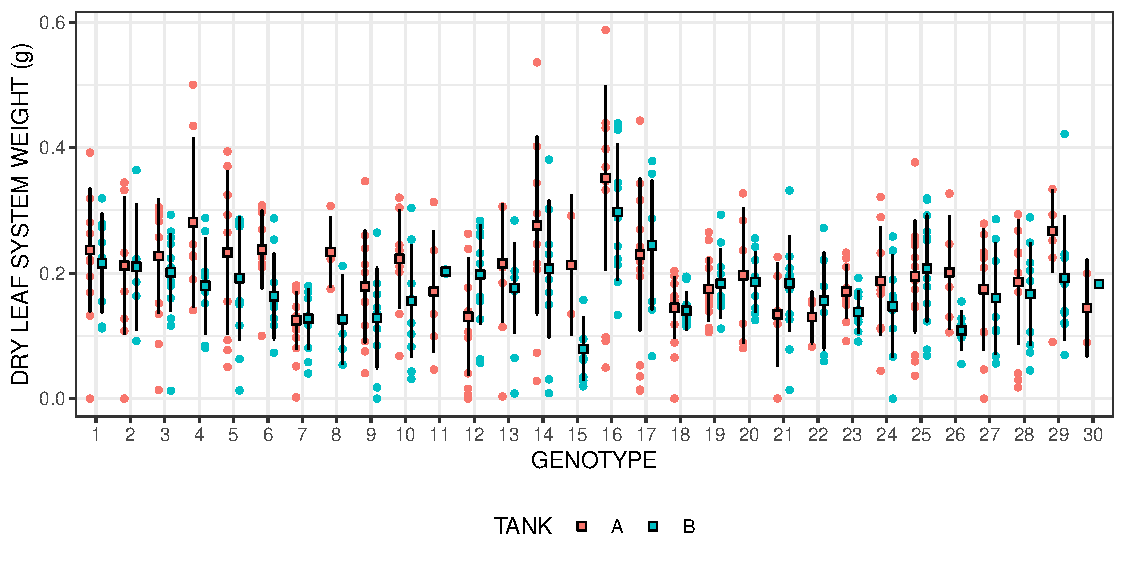
\includegraphics[width = \textwidth]{../../Figures/DRY_LS_summary_plot.pdf}
		\caption{Dry leaf weight ($DRY\_LS$)}
	\end{subfigure}

	\begin{subfigure}[t]{\textwidth}
		\centering
		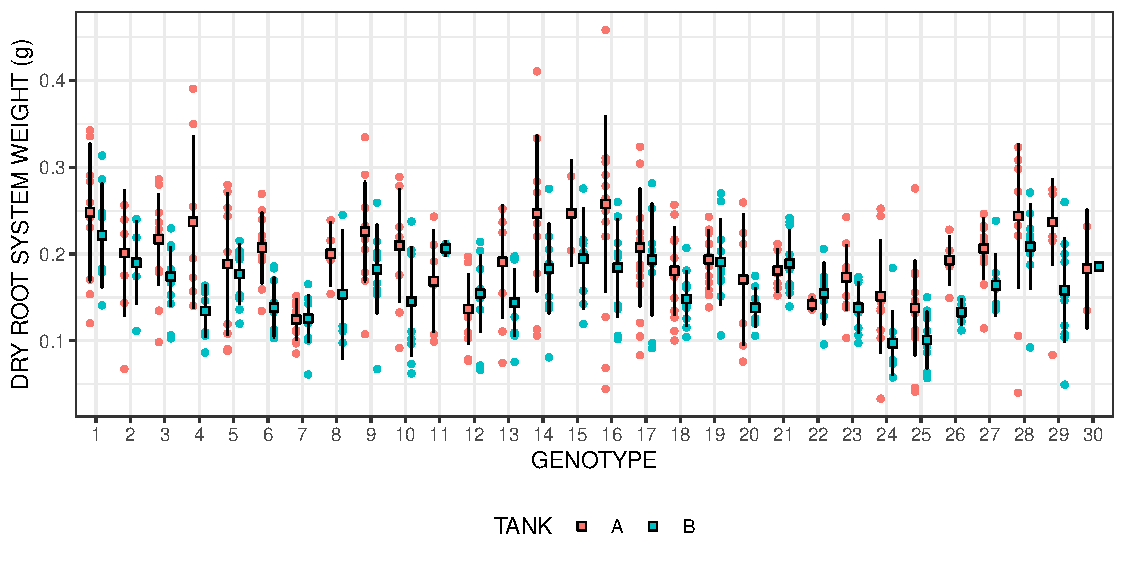
\includegraphics[width = \textwidth]{../../Figures/DRY_RS_summary_plot.pdf}
		\caption{Dry root weight ($DRY\_RS$)}
	\end{subfigure}
	\caption[Dotplot of the mean weight and associated standard deviation]{Dotplot displaying mean weight (\protect\emptysquare) and associated standard deviation (\protect\blackline), grouped by tanks for each variable.}
\end{figure}
\begin{figure}\ContinuedFloat
	\captionsetup[figure]{list=no}
	\begin{subfigure}[t]{\textwidth}
		\centering
		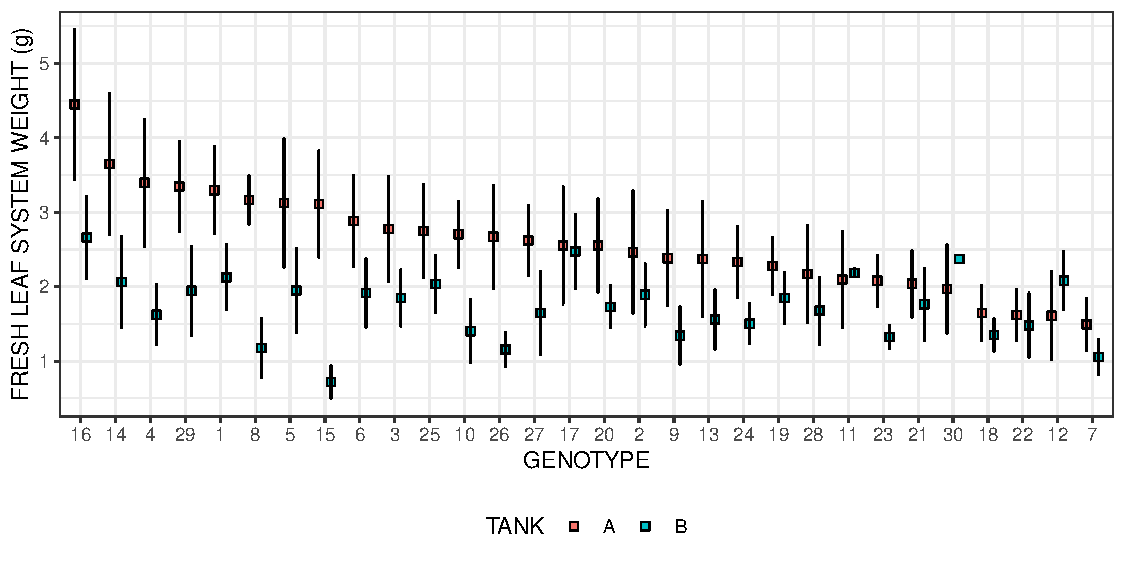
\includegraphics[width = \textwidth]{../../Figures/FRESH_LS_summary_plot.pdf}
		\caption{Fresh leaf weight ($FRESH\_LS$)}
	\end{subfigure}

	\begin{subfigure}[t]{\textwidth}
		\centering
		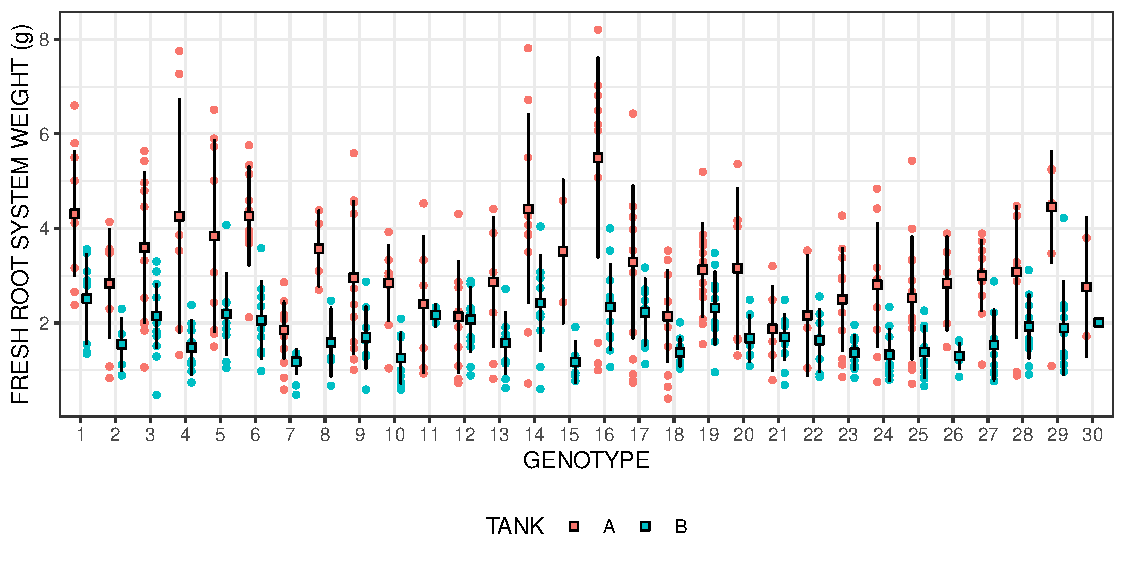
\includegraphics[width = \textwidth]{../../Figures/FRESH_RS_summary_plot.pdf}
		\caption{Fresh root weight ($FRESH\_RS$)}
	\end{subfigure}
	\caption[Dotplot of the mean weight and associated standard deviation]{Dotplot displaying mean weight (\protect\emptysquare) and associated standard deviation (\protect\blackline), grouped by tanks for each variable.}
	\label{fig:dotplot_all_variables}
\end{figure}

\section{SpATS analysis}
The SpATS model usually takes rows and columns coordinates as inputs for spatial position. Given that we have tanks (A and B), strips (from 1 to 99) and positions (from 1 to 5), we reshaped the data to give have the tank side by side and the 99 strips divided in two columns (to have a similar disposition to the one in the greenhouse). Figure \ref{fig:tank_disposition} shows the reshaping of the positions. This new display of the data allows us to see the difference between tanks more clearly and to visualize the variables' values as they were in the greenhouse.

\begin{figure}[hbtp]
	\centering
	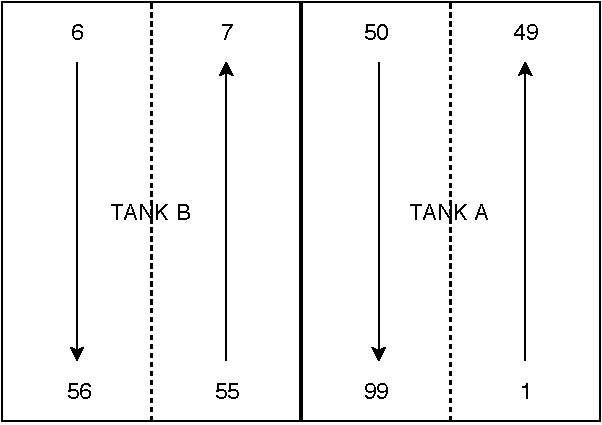
\includegraphics[scale = 0.7]{figures/TANK_repartition.pdf}
	\caption[Reshaping of the data table to fit the disposition of the greenhouse]{Reshaping of the data table to fit the 
	disposition of the greenhouse. The number indicates the original strip number.}
	\label{fig:tank_disposition}	
\end{figure}

The model was then fitted for the four weight variables, using the settings specified in the previous chapter. Table \ref{tab:spats_dimensions} presents the effective dimensions associated with the bivariate smooth surface components (see equation \ref{eq:full_bivariate_smooth_surface_model}) 
and their relative contribution to the fitted surface for each variable.
We see that the fresh weights exhibited a higher complexity in the structure of the spatial surface. This is reflected by the higher value of contribution for the smooth-by-smooth term ($f_{u, v}(\boldsymbol{u}, \boldsymbol{v})$), that accounts for almost 70\% in both variables. Besides this term, the main sources of variation are the linear (for the strips) by smooth (for the positions) term and the smooth trend along the strips term. It is not surprising to have more variation along the strips than along the positions given that there were 99 strips but only 5 positions.
Concerning the dry weights, the variation is more spread between all the components for both variables. This means that the variation in the data can be more easily attributed to the strips and positions of the plants. However, all the variables have components with zero value of $ED_{s}$\footnote{the actual values were not zero but it is denoted as such since they were inferior to $1 \times 10^{-15}$}, indicating that these terms were not necessary to model the spatial surface.\\

% Table generated by Excel2LaTeX from sheet 'Sheet2'
\begin{table}[htbp]
  \rowcolors{2}{gray!25}{white}
  \centering
  \caption[Effective dimensions of the SpATS model]{Model dimensions and effective dimensions (and percentage of the total of 
  the spatial components) of each spatial components for all variables. $ED_{\epsilon}$ represents the effective dimensions for 
  the residuals; $ED_{g}$, is the effective dimensions for the genotype and $H_{g}^2$ is the heritability. Here $\mathbf{v}$ 
  represents the columns, i.e. the position on the strip; and $\mathbf{u}$ represents the rows, i.e. the strip itself.}
    \begin{tabular}{lrrrrr}
    \toprule
    \begin{tabular}[b]{@{}l@{}}Model \\ components\end{tabular} & \multicolumn{1}{c}{Model} & \multicolumn{1}{l}{FRESH\_LS} & \multicolumn{1}{l}{FRESH\_RS} & \multicolumn{1}{l}{DRY\_LS} & \multicolumn{1}{l}{DRY\_RS} \\
    \midrule
    $f_{v}(\mathbf{v})$ & 6     & 0 (0,00\%) & 0 (0,00\%) & 0 (0,00\%) & 0 (0,00\%) \\
    $f_{u}(\mathbf{u})$ & 100   & 0,8 (8,73\%) & 2,26 (14,10\%) & 1,02 (17,26\%) & 1,8 (17,26\%) \\
    $\boldsymbol{u} \odot h_{v}(\boldsymbol{v})$ & 6     & 1,84 (19,95\%) & 2,63 (16,40\%) & 1,47 (24,77\%) & 2,54 (24,77\%) \\
    $\boldsymbol{v} \odot h_{u}(\boldsymbol{u})$ & 100   & 0,24 (2,56\%) & 0 (0,00\%) & 1,09 (18,36\%) & 0,49 (18,36\%) \\
    $f_{u, v}(\boldsymbol{u}, \boldsymbol{v})$ & 150   & 6,33 (68,76\%) & 11,16 (69,50\%) & 2,35 (39,62\%) & 0,08 (39,62\%) \\
    Total & 362 & 9,21 (100\%) & 16,15 (100\%) & 5,93 (100\%)& 4,91 (100\%)\\
    \midrule
    $ED_{\epsilon}$ &       & 466.6 & 459,3 & 470,2 & 470,1 \\
    \midrule
    $ED_{g}$  & 30    & 21,02 & 22,58 & 21,38 & 22,98 \\
    $H_{g}^2$ &       & 0,72  & 0,78  & 0,74  & 0,79 \\
    \bottomrule
    \end{tabular}%
  \label{tab:spats_dimensions}%
\end{table}%

Table \ref{tab:spats_dimensions} also presents the effective dimension of the genetic component ($ED_{g}$) which is quite similar across variables. This is reflected in the heritability values which are all around 75\%. However, it should be noted that the SpATS model tends to overestimate the heritability \parencite{rodriguez-alvarez_spatial_2016}. This means that a good part of the phenotypic variation can be attributed to genotypes.\\

Figure \ref{fig:spats_model_results} shows the raw data ($\mathbf{a}$), a graphical representation of the fitted spatial trend ($f(\boldsymbol{u}, \boldsymbol{v})$) ($\mathbf{b}$) and the spatially independent residuals $\boldsymbol{\epsilon}$ ($\mathbf{c}$) obtained from the SpATS package. While there are a lot of missing data, someone spatial trends still stand out. Just as predicted with the dotplot in the descriptive statistics section, weights in the B tank are lower than in the A tank. This is especially visible for the fresh weight, where the total weight range is greater than for the dry weights.\\

The inspection of the fitted spatial surfaces shows us that the trends have been captured by the SpATS model. An additional analysis of the residuals suggests that the spatial patterns have effectively been removed in all four variables by the tow-dimensional spline surface. However, some high data points still persists in the residuals, this is mainly due to the high variability of the weights in the raw data. In order to fully analyse the residuals, two additional diagnosis plots have been created: a lagplot to test for spatial independence and a normal distribution to test for the normality assumption. These plots are presented in appendix \ref{appendix:residuals}. Overall, the residuals seem to be independent and normally distributed, which confirms again that the spatial pattern has been well-captured by the model. Another interesting tool to evaluate the spatial independence is the variogram, presented in the previous chapter (section \ref{sec:arxar_model}). 
As said previously, if the model for spatial trend fits well, the variogram should be a horizontal plane \parencite{piepho_linear_2010}.\\

\begin{table}[ht]
\centering
\rowcolors{2}{gray!25}{white}
\caption{Individual variances of all the components of the SpATS model.} 
\begin{tabular}{lrrrr}
  \toprule
 & FRESH\_LS & FRESH\_RS & DRY\_LS & DRY\_RS \\ 
  \midrule
$\mathbf{c}_{g}$ & 1.71E-01 & 2.62E-01 & 1.27E-03 & 6.90E-04 \\ 
  $\mathbf{c}_{v}$ & 3.24E-03 & 5.08E-03 & 1.95E-07 & 8.47E-17 \\ 
  $\mathbf{c}_{u}$ & 1.86E-04 & 2.25E-05 & 2.42E-07 & 3.93E-08 \\ 
  $f_{v}(\mathbf{v})$ & 2.20E+01 & 1.10E+02 & 1.06E-04 & 2.65E-01 \\ 
  $f_{u}(\mathbf{u})$ & 2.75E-05 & 5.36E-05 & 5.40E-08 & 1.55E-08 \\ 
  $\boldsymbol{u} \odot h_{v}(\boldsymbol{v})$ & 5.60E-52 & 1.76E-38 & 1.51E-52 & 1.44E-13 \\ 
  $\boldsymbol{v} \odot h_{u}(\boldsymbol{u})$ & 1.81E-09 & 4.83E-04 & 6.75E-10 & 1.43E-06 \\ 
  $f_{u, v}(\boldsymbol{u}, \boldsymbol{v})$ & 3.98E-01 & 2.52E-01 & 6.13E-05 & 7.13E-04 \\ 
  $\epsilon$ & 4.707E+01 & 5.014E+01 & 3.364E-02 & 1.219E-02\\
   \bottomrule
\end{tabular}
\label{tab:spats_variances}
\end{table}

Finally, another interesting result from figure \ref{fig:spats_model_results} is the comparison between the scales of spatial variations and residual variations, because they provide an idea of the relative importance of field trends for each variable. We see that for all variables, the scales of the residuals are about ten-fold the scales of the fitted surfaces. This is explained by the effective dimension of the residuals presented in table \ref{tab:spats_dimensions}. We see that, for all variables, those dimensions are much higher than the others. This means that the spatial variation was lower than the random variation, and even though spatial patterns were captured, much of the variation is still present in the residuals of the models. Given that the raw data present a high variability and a lot of missing values, we expected to have residuals with high variance (see table \ref{tab:spats_variances} for the variances linked to each component of the model).

\begin{figure}
	\begin{subfigure}[t]{\textwidth}
		\centering
		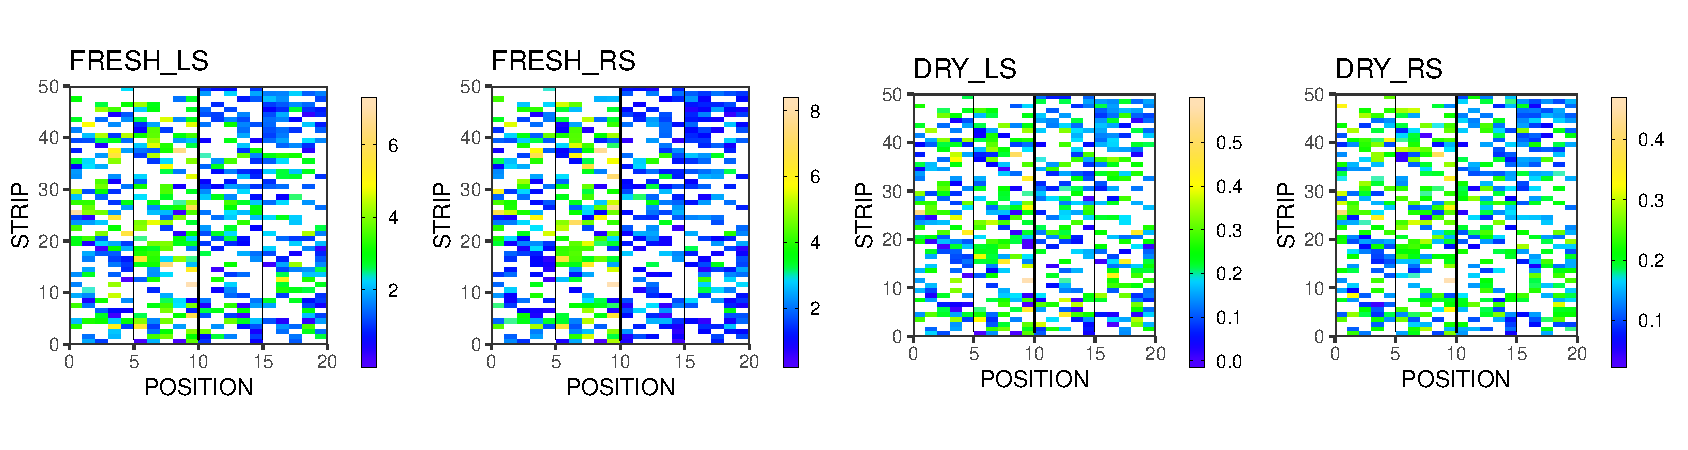
\includegraphics[width = \textwidth]{../../Figures/rawData_plot.pdf}
		\caption{Raw data}
	\end{subfigure}
	
	\begin{subfigure}[t]{\textwidth}
		\centering
		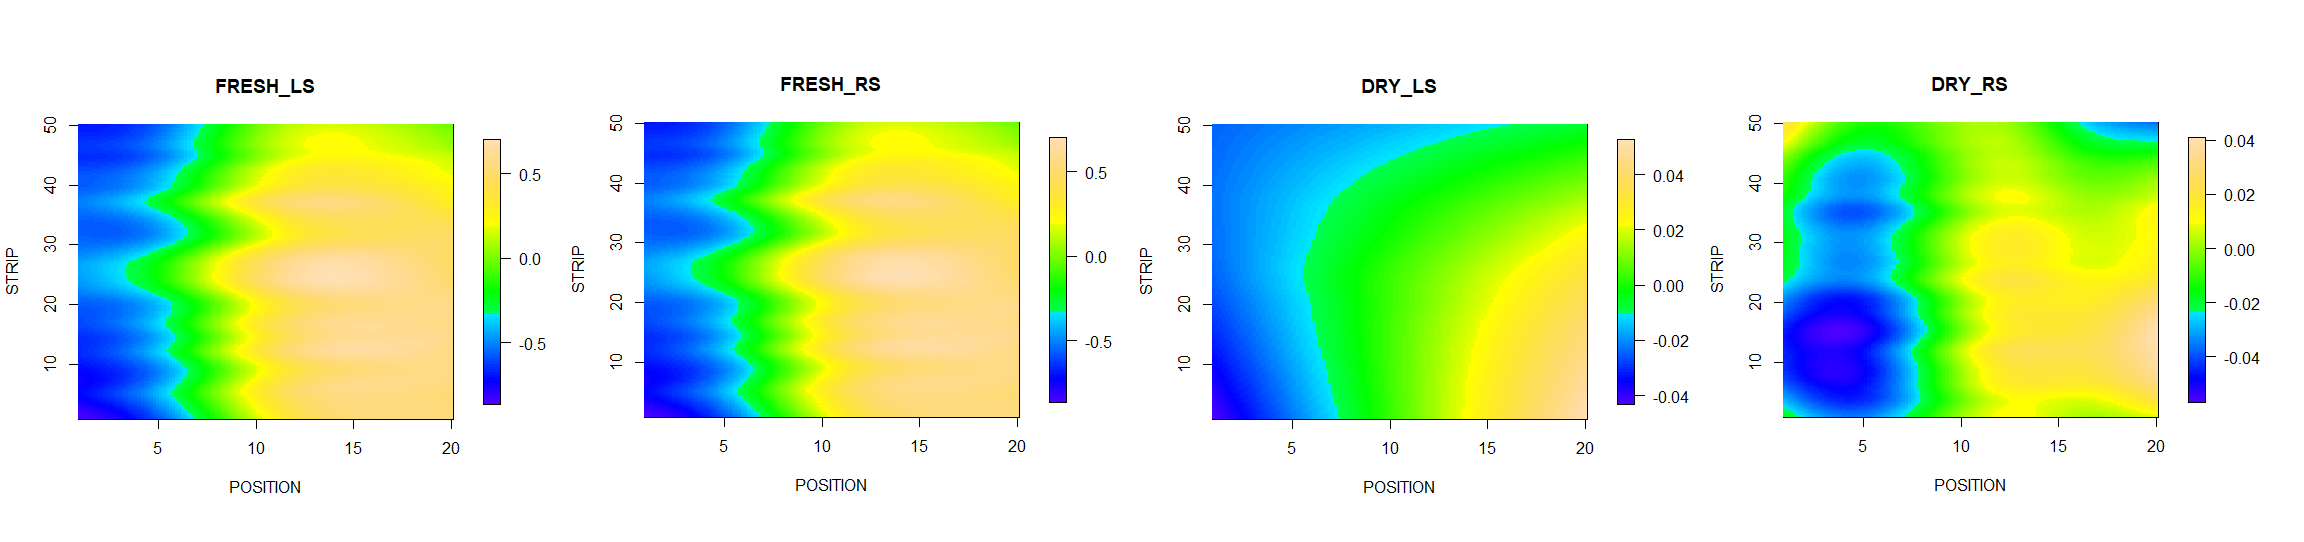
\includegraphics[width = \textwidth]{../../Figures/fitted.png}
		\caption{Fitted spatial trend}
	\end{subfigure}
	
	\begin{subfigure}[t]{\textwidth}
		\centering
		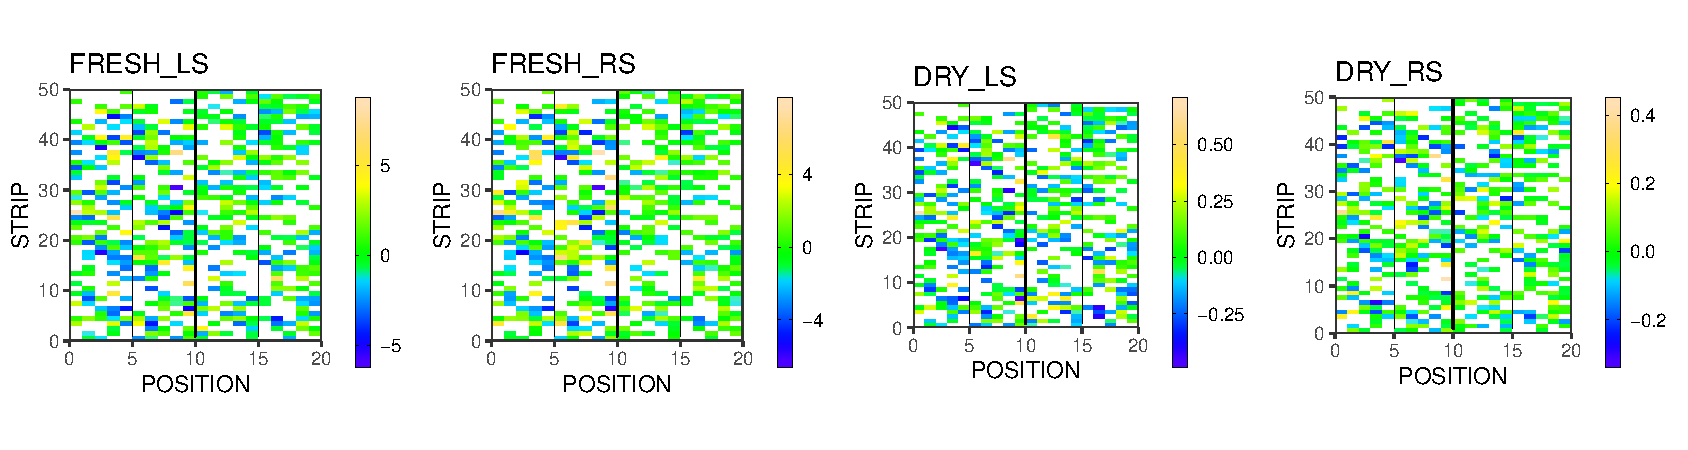
\includegraphics[width = \textwidth]{../../Figures/residuals_plot.pdf}
		\caption{Residuals' spatial plot}
	\end{subfigure}
	\caption{Raw data, fitted spatial trend and residuals' plot for each variable.}
	\label{fig:spats_model_results}
\end{figure}

\section{ARxAR model analysis}
\section{Model comparison}
%\subsection{Performances}
%\subsection{Parametrization}
%\subsection{Modelling strategy}


%Conclusion
\chapter{Conclusion}
%Conclusion
Goal of thesis not well met since unused data and untapped potential variables + not time evolution taken into account.

Spatial model unfit to moving environement but this environement was better for the platform.
However this could have been detected with GLMs.

Useful to compare to other trials with same genotypes and other trials on platform to if patterns are picked up.

No visible gradient on position

\clearpage


%% Bibliography %%
\printbibliography

%% Appendix %%
\begin{appendices}
\addcontentsline{toc}{chapter}{Appendix} %adds it to the table of contents
\chapter{Additional informations on computation}
\label{appendix:add_info}
\section{Element-wise product}
\label{appendix:add_info_element_wise_product}
The element-wise product between two matrix $\mathbf{A}$ and $\mathbf{B}$ is noted $\mathbf{A} \odot \mathbf{B}$ and is defined in the following way:\\
For two matrices $\mathbf{A}$, $\mathbf{B}$ of same dimensions $n \times m$, the element-wise product is a $n \times m$ matrix where the elements are defined by:
\[(\mathbf{A} \odot \mathbf{B})_{i,j} = (\mathbf{A})_{i,j} \cdot (\mathbf{B})_{i,j}\]
The product is undefined for matrices of different dimensions

\section{Kronecker product}
\label{appendix:add_info_kronecker_product}
The Kronecker product of two matrix $\mathbf{A}$ and $\mathbf{B}$ of respective dimensions $n \times m$ and $p \times q$ is a $np \times mq$ block matrix where the elements are defined by:
\[\mathbf { A } \otimes \mathbf { B } = 
\left[ 
\begin{array}
 { c c c } { a _ { 11 } \mathbf { B } } & { \cdots } & { a _ { 1 n } \mathbf { B } } \\ { \vdots } & { \ddots } & { \vdots } \\ { a _ { m 1 } \mathbf { B } } & { \cdots } & { a _ { m n } \mathbf { B } } 
\end{array} 
\right]\] 

\section{Polynomials splines}
\label{appendix:polynomial_splines}
\textcite{fahrmeir_regression:_2013} state that a function $f : [ a , b ] \rightarrow \mathbb { R }$ is called a polynomial spline of degree $l \geq 0$ with knots $a = \kappa _ { 1 } < \ldots < \kappa _ { m } = b$, if it fulfills the following conditions:
\begin{enumerate}
\item $f(z)$ is $(l-1)$ times continuously differentiable. The special case of $l = 1$ corresponds to $f(z)$ being continuous (but not differentiable). We do not state any smoothness requirements for $f(z)$ when $l=0$.
\item $f(z)$ is a polynomial of degree $l$ on intervals $\left[ \kappa _ { j } , \kappa _ { j + 1 } \right)$ defined by the knots.
\end{enumerate}
Moreover, it can be shown that each polynomial spline of degree $l$ with
knots $\kappa _ { 1 } < \ldots < \kappa _ { m }$ can be uniquely determined as a linear combination of the $d = l+m-1$ functions
$B_1, \dots , B_d$, called the \textit{basis functions}, since we can uniquely represent all polynomials splines by using these functions.

\subsection{B-splines}
B-splines are polynomial splines with specific basis functions. B-spline basis functions are constructed
from piecewise polynomials that are fused smoothly at the knots to achieve the desired smoothness constraints. More specifically, a B-spline basis function consists
of $(l+1)$ polynomial pieces of degree $l$ , which are joined in an $(l-1)$ continuously differentiable way. All B-spline basis functions are set up based on a given knot configuration. Using the complete basis, the function $f(z)$ can again be represented through a linear combination of $d = m + l-1$ basis
functions, i.e.,
\[f ( z ) = \sum _ { j = 1 } ^ { d } \gamma _ { j } B _ { j } ( z )\text{.}\]
The B-splines of order $l=0$ can be written as
\[B _ { j } ^ { 0 } ( z ) = \left\{ \begin{array} { l l } { 1 } & { \kappa _ { j } \leq z < \kappa _ { j + 1 } } \\ { 0 } & { \text { otherwise } } \end{array} \right. \quad j = 1 , \ldots , d - 1\]
and the B-splines for higher order $l$ can be written as
\[B _ { j } ^ { l } ( z ) = \frac { z - \kappa _ { j - l } } { \kappa _ { j } - \kappa _ { j - l } } B _ { j - 1 } ^ { l - 1 } ( z ) + \frac { \kappa _ { j + 1 } - z } { \kappa _ { j + 1 } - \kappa _ { j + 1 - l } } B _ { j } ^ { l - 1 } ( z ) \text{.}\]
The estimation of a polynomial spline in B-spline representation can be traced back to the estimation of a linear model with a large number of parameters and design matrix 
\[\mathbf{Z}= \left( \begin{array} { c c c } { B _ { 1 } ^ { l } \left( z _ { 1 } \right) } & { \dots } & { B _ { d } ^ { l } \left( z _ { 1 } \right) } \\ { \vdots } & { } & { \vdots } \\ { B _ { 1 } ^ { l } \left( z _ { n } \right) } & { \dots } & { B _ { d } ^ { l } \left( z _ { n } \right) } \end{array} \right) \text{.} \]
The linear combination of basis functions can then be written in matrix form
\[ \mathbf{y} = \mathbf{Z} \mbox{\boldmath$\gamma$} \]
where the coefficient matrix, {\boldmath$\gamma$} can be estimated using least squares.\\
The estimation of a B-spline fit can be summarized in three steps:
\begin{enumerate}
\item We calculate a complete B-spline basis for a given number of knots.
\item The least squares estimate {\boldmath$\hat{\gamma}$} yields an amplitude $\hat{\gamma_j}$ for the scaling of every basis function.
\item We obtain the final estimate by summing the scaled basis function.
\end{enumerate}

\subsection{Penalized splines}
We clearly see that the quality of the estimation by polynomials splines highly depends on the number of knots and that this can easily lead to an over-fitting issue. To overcome this problem, \textit{penalized splines (P-splines)} introduce a roughness penalty term that prevents over-fitting and minimize a \textit{penalized least squares (PLS) criterion} instead of the usual least squares criterion.\\
To characterize the smoothness of any type of function, the
use of (squared) derivatives is appropriate, since these represent measures for the variability of a function. Therefore penalties based on the second derivative, such as
\[ \lambda \int \left( f ^ { \prime \prime } ( z ) \right) ^ { 2 } d z\text{,} \]
are particularly attractive since they measure the curvature of a function. Since we know that the first derivative of a B-spline can be written as a function of the first differences of the corresponding coefficient vector, we can use differences of a higher order $r$ if we aim at a smooth function in terms of $r$th-order derivatives. This leads to the penalized residual sum of squares
\[\operatorname { PLS } ( \lambda ) = \sum _ { i = 1 } ^ { n } \left( y _ { i } - \sum _ { j = 1 } ^ { d } \gamma _ { j } B _ { j } \left( z _ { i } \right) \right) ^ { 2 } + \lambda \sum _ { j = r + 1 } ^ { d } \left( \Delta ^ { r } \gamma _ { j } \right) ^ { 2 }\text{,}\]
where $\Delta^r$ denotes the $r$th-order differences.The smoothing parameter $\lambda \geq 0$ controls the compromise between fidelity to the data and smoothness of the resulting function estimate. The PLS criterion can be rewritten using matrix notation
\[ \operatorname { PLS } ( \lambda ) = ( \mathbf{y} - \mathbf{Z} \boldsymbol{\gamma} ) ^ { \prime } (  \mathbf{y} - \mathbf{Z} \boldsymbol{\gamma}) + \lambda \boldsymbol{\gamma} ^ { \prime }\mathbf{K_r} \boldsymbol{\gamma} \]
where $\mathbf{K_r}$ is the $r$th-order difference penalty matrix, and can be decomposed as $\mathbf{D_r}\prime \mathbf{D_r}$ with $D_r$ the $r$th-order difference matrix.
The smoothing parameter $\lambda \geq 0$ controls the compromise between fidelity to the data and smoothness of the resulting function estimate. The PLS estimate of the coefficient matrix is then 
\[ \hat { \boldsymbol{\gamma} } = \left(\mathbf{ Z} ^ { \prime } \mathbf {Z} + \lambda \mathbf{K} \right) ^ { - 1 }\mathbf{ Z} ^ { \prime }\mathbf{ y} \text{.}\]
For more detailed information about polynomials splines, please refer to \textcite{fahrmeir_regression:_2013} and \textcite{eilers_flexible_1996}

\section{Penalized form of the solution and smoothing parameter selection}
\label{appendix:SpATS_add_comput_info}
Let us consider the model only containing a bivariate smooth surface and an error term:
\[
	    y _ { i } = f \left( u _ { i } , v _ { i } \right) + \varepsilon _ { i } , \text { with } \varepsilon _ { i } \sim N 
	    \left( 0 , \sigma ^ { 2 } \right) \text{.} 
	    \]
It can be rewritten, in matrix notation, as the tensor product of B-splines:
\[
    \boldsymbol{y} = \boldsymbol{B}\boldsymbol{\alpha} + \boldsymbol{\epsilon}
    \text{.}
\]
Since the model is purely parametric, it can be estimated by minimizing the residual sum of squares (with explicit solution $\Hat{\boldsymbol{\alpha}} = (\mathbf{B}^t\mathbf{B})^{-1}\mathbf{B}^t\mathbf{y}$). To prevent over-fitting, \textcite{eilers_flexible_1996} propose to incorporate a discrete penalty on the coefficient associated to adjacent B-splines. For the two-dimensional case, the vector $\boldsymbol{\alpha}$ can be seen as an  $(L \times P)$  matrix  of  coefficients, $\mathbf{A}=[\alpha_{lp}]$. Now the rows  and columns of $\mathbf{A}$ correspond to the regression coefficients in the $v$ and  $u$ direction, respectively. In anisotropic (direction-dependant) P-splines, a different amount of smoothing is assumed along the $u$ and $v$ directions. It leads to two penalties:  one on all rows of $\mathbf{A}$,  the other on all of its columns; and the penalized least squares objective function becomes \parencite{eilers_multivariate_2003}
\[
\begin{aligned}
    S^{*} & = \underbrace{\|\boldsymbol{y}-\boldsymbol{B} \boldsymbol{\alpha}\|^{2}}_{\text{Original objective function}} \\
    	  & +\underbrace{\invbreve{\lambda}\|\invbreve{\boldsymbol{D}} A\|_{F}^{2}}_{\text{Penalty along the columns}} \\
    	  & +\underbrace{\breve{\lambda}\left\|\boldsymbol{A} \breve{D}^{t}\right\|_{F}^{2}}_{\text{Penalty along the rows}} \\
    =	  & \|\boldsymbol{y}-\boldsymbol{B} \boldsymbol{\alpha}\|^{2}+\boldsymbol{\alpha}^{t} \boldsymbol{P} \boldsymbol{\alpha}
    \text{,}
\end{aligned}
\]
where $\boldsymbol{P}=\invbreve{\lambda}\left(\boldsymbol{I}_{P} \otimes \invbreve{\boldsymbol{D}}^{t} \invbreve{\boldsymbol{D}}\right)+\breve{\lambda}\left(\breve{\boldsymbol{D}}^{t} \breve{\boldsymbol{D}} \otimes \boldsymbol{I}_{L}\right)$ is the penalty matrix, $\invbreve{\lambda}$ and $\breve{\lambda}$ are the smoothing parameters acting, respectively, on the columns and rows of $\mathbf{A}$, and $\invbreve{\mathbf{D}}$ and $\breve{\mathbf{D}}$ are the matrices that form differences of order $d_u$ and $d_v$ respectively. The minimizer of the starting equation then becomes 
\[
    \widehat{\boldsymbol{\alpha}}=\left(\boldsymbol{B}^{t} \boldsymbol{B}+\boldsymbol{P}\right)^{-1} \boldsymbol{B}^{t} 
    \boldsymbol{y}
    \text{,}
\]
which is the penalized form of the solution. However, $\boldsymbol{P}$ is rank-deficient.
To have a full rank penalty matrix, the key is to rewrite the model and setting
\[
    \mathbf{B}\boldsymbol{\alpha} = \boldsymbol{X}_{s} \boldsymbol{\beta}_{s}+\boldsymbol{Z}_{s} \boldsymbol{c}_{s}
    \text{.}
\]
There are now two bases: $\mathbf{X}_{s}$, with coefficients that are not penalized at all, and $\mathbf{Z}_{s}$, with a size 
penalty on its coefficients. This decomposition follows the proposal by \textcite{lee_p-spline_2011}, based on eigenvalue 
decomposition which gives rise to a diagonal penalty matrix.\\

The two bases have the following structures:
\begin{equation*}
\boldsymbol{X}_{s}=\left[\mathbf{1}_{n}, \boldsymbol{u}, \boldsymbol{v}, \boldsymbol{u} \odot \boldsymbol{v}\right]
    \quad
    \text{and}
    \quad
    \mathbf{Z}_{s}=\left[\mathbf{Z}_{v}, \mathbf{Z}_{u}, \mathbf{Z}_{v} \boxdot \mathbf{u}, \mathbf{v} \boxdot \mathbf{Z}_{u}, 
    \mathbf{Z}_{v} \boxdot \mathbf{Z}_{u} \right]
    \text{,}
\end{equation*}
where $\boldsymbol{u}$ and $\boldsymbol{v}$ are still, respectively, the vectors of row and column positions. 
Here $\mathbf{Z}_{u}$ and $\mathbf{Z}_{v}$ are penalized version of the B-splines basis $\breve{\mathbf{B}}$ (rows) and
$\invbreve{\mathbf{B}}$ (columns). This new way of writing the problem leads to another penalty matrix 
$ \widetilde{\boldsymbol{P}}$, which is a block diagonal matrix. Each block of $ \widetilde{\boldsymbol{P}}$ corresponds to a 
block in $\mathbf{Z}_{s}$. Similarly to $\boldsymbol{P}$, the penalty matrix of the previous section, this new penalty matrix 
only depends on the two tuning parameters $\invbreve{\lambda}$ (smoothing along the columns) and $\breve{\lambda}$ (smoothing 
along the rows).
Figure \ref{fig:matrix_diagram} presents a diagram clarifying the structures and relations of the different matrices presented 
throughout this section.\\

This reformulation provides the ANOVA type decomposition discussed in the previous section 
(\ref{eq:full_bivariate_smooth_surface_model}), and explains how the bilinear smooth surface can be modelled using P-splines and 
tensor products of P-splines.
The block structure of $\mathbf{X}_s$ and $\mathbf{Z}_s$ implies
\[
    \begin{aligned} 
        f(\boldsymbol{u}, \boldsymbol{v}) & =\boldsymbol{X}_{s} \boldsymbol{\beta}_{s}+Z_{s} \boldsymbol{c}_{s} \\ 
        								  & =\mathbf{1}_{n} \beta_{0}+\boldsymbol{u} \beta_{1}+\boldsymbol{v} \beta_{2}+
        								  \boldsymbol{u} \odot \boldsymbol{v} \beta_{3} \\
        								  & + \underbrace{f_{v}(\boldsymbol{v})}_{\boldsymbol{Z}_{v} \boldsymbol{c}_{s 1}}+
        								  \underbrace{f_{u}(\boldsymbol{u})}_{\boldsymbol{Z}_{u} \boldsymbol{c}_{s 2}} +
        								  \underbrace{\boldsymbol{u} \odot h_{v}(\boldsymbol{v})}_{\left[\boldsymbol{Z}_{v} 
        								  \square \boldsymbol{u}\right] \boldsymbol{c}_{s 3}}+\underbrace{\boldsymbol{v} \odot 
        								  h_{u}(\boldsymbol{u})}_{\left[\boldsymbol{v} \square \boldsymbol{Z}_{u}\right] 
        								  \boldsymbol{c}_{s 4}} +\underbrace{f_{u, v}(\boldsymbol{u}, \boldsymbol{v})}
        								  _{\left[\boldsymbol{Z}_{v} \square \boldsymbol{Z}_{u}\right] \boldsymbol{c}_{s 5}}
        								  \text{,}
    \end{aligned}
\]
where $\boldsymbol{c}_{sk} \ (k = 1,\ldots,5)$ contains the elements of $\boldsymbol{c}_s$ that correspond to the $k$th block of $\boldsymbol{Z}_s$, i.e. $\boldsymbol{c}_s = (\boldsymbol{c}_{s1}^t,\ldots,\boldsymbol{c}_{s5}^t)^t$. The details about the specific block component of $\boldsymbol{Z}_s$ and the computation of the new penalty matrix are available in  \textcite{rodriguez-alvarez_correcting_2018} and the appendices therein.\\

Therefore, using this new notation, model (\ref{eq:smooth_part_only_model}) that only contains a smooth bivariate surface and an error term can be rewritten in the following way:

\[
    \boldsymbol{y}=\boldsymbol{X}_{s} \boldsymbol{\beta}_{s}+\boldsymbol{Z}_{s} \boldsymbol{c}_{s}+\boldsymbol{\varepsilon}, 	
    \text { with } 
    \boldsymbol{\varepsilon} \sim N\left(\mathbf{0}, \sigma^{2} \boldsymbol{I}_{n}\right) 
    \text { and } 
    \boldsymbol{c}_{s} \sim N\left(\mathbf{0}, \boldsymbol{G}_{s}\right)
    \text{,}
\]
where $\boldsymbol{G}_{s} = \sigma^2\widetilde{\boldsymbol{P}}^{-1}$ and also has a block diagonal structure, similar to that of $\widetilde{\boldsymbol{P}}$ (this structure is also represented on 
figure \ref{fig:matrix_diagram}). 
However, $\boldsymbol{G}_{s}$ depends on two different parameters, $\breve{\sigma}^2 =\sigma / \breve{\lambda}$ and $
\invbreve{\sigma}^2 =\sigma / \invbreve{\lambda}$, which are variance parameters. 
As shown in the diagram in Figure \ref{fig:matrix_diagram}, the same variance parameters control the smoothness of the both the 
main effects and interactions terms. 
This prevents the use of standard mixed models software for estimation since $\mathbf{G}_s$ has its last block depending on both 
$\breve{\sigma}^2$ and $\invbreve{\sigma}^2$, but in a non-linear way. 
Even though \textcite{rodriguez-alvarez_fast_2015} presented a specialized algorithm to deal with this issue, 
here the PS-ANOVA decomposition approach \parencite{lee_efficient_2013} is used to allow the use of standard mixed model estimation procedures. \textcite{lee_efficient_2013} therefore propose to use a different variance component for each smooth component in $\mathbf{G}_s$, thus redefining this matrix as a linear function of variance parameters:
\[
    \boldsymbol{G}_{s} = 
%	\bigoplus_{k=1}^{5} \sigma_{s k}^{2} \Lambda_{s k} =
    \bigoplus_{k=1}^{5} \boldsymbol{G}_{s k}= 
    \text{ blockdiag }
    \left(\boldsymbol{G}_{s 1}, \boldsymbol{G}_{s 2}, \boldsymbol{G}_{s 3}, \boldsymbol{G}_{s 4}, \boldsymbol{G}_{s 5}\right)
    \text{,}
\]
where $\boldsymbol{G}_{s k}$ %= \sigma_{sk}^2\boldsymbol{\Lambda}_{sk} \ (k=1,\ldots,5)$
is the $k$th block of the $\mathbf{G}_{s}$ matrix, depending on the specific variance component $\sigma_{sk}^2$. 
In other words, here the tensor product P-splines mixed model is represented as the sum of 5 sets of mutually independent Gaussian random components $\mathbf{c}_{sk}$, each depending on one variance $\sigma_{sk}^2 \ (k=1,\ldots,5)$.\\

Within this mixed model framework, the smoothing parameters, defined earlier as the ratio between the residual variance and the
corresponding variance effect $\lambda_{sk} = \sigma^2_{e} / \sigma^2_{sk}$, are determined by restricted maximum likelihood (REML). Therefore the smoothness of the spatial surface is tuned by five distinct parameters, applying anisotropic (direction-dependant) smoothing. This parametrization provides flexibility to account for both global and local variations in the field. Furthermore, the decomposition of $f(\boldsymbol{u},\boldsymbol{v})$ enables a more explicit interpretation of the main patterns of spatial variation \parencite{rodriguez-alvarez_correcting_2018}.

% Redefine the main unit
\newcommand{\myunit}{1 cm}

\begin{figure}
\centering
\resizebox{\columnwidth}{!}{%
\begin{tikzpicture}[>=latex]

% Matrix
\matrix (xs) [matrix of math nodes,%
             left delimiter  = (,%
             right delimiter = )] at (-0.5,5*\myunit)
{%
  1_n   \\
  \mathbf{u}    \\
  \mathbf{v}    \\
  \mathbf{u} \odot \mathbf{v} \\
};
\node [draw,below=10pt] at (xs.south) 
    {$\mathbf{X}_{s}$};

% Matrix annotations
\node [anchor=west] at (0.5,5.8) {\textit{Intercept}};
\node [anchor=west] at (0.5,5.3) {\textit{Cols}};
\node [anchor=west] at (0.5,4.8) {\textit{Rows}};
\node [anchor=west] at (0.5,4.3) {\textit{Cols $\times$ Rows}};


% Matrix
\matrix (bs) [matrix of math nodes,%
             left delimiter  = (,%
             right delimiter = )] at (4.5*\myunit,5*\myunit)
{%
  \beta_{1} \\
  \beta_{2} \\
  \beta_{3} \\
  \beta_{4} \\
};
\node [draw,below=10pt] at (bs.south) 
    {$\boldsymbol{\beta}_{s}$}; 


% Matrix
\matrix (zs) [matrix of math nodes,%
             left delimiter  = (,%
             right delimiter = )] at (7*\myunit,5*\myunit)
{%
  Z_{v} \\
  Z_{u} \\
  \mathbf{u} \boxdot Z_{v} \\
  \mathbf{v} \boxdot Z_{u} \\
  Z_{u} \boxdot Z_{v} \\
};
\node [draw,below=10pt] at (zs.south) 
    {$\mathbf{Z}_{s}$};

% Matrix annotation
\node [anchor=west] at (8.2,6.2) {\textit{Smooth cols trend}};
\node [anchor=west] at (8.2,5.6) {\textit{Smooth rows trend}};
\node [anchor=west] at (8.2,5) {\textit{Linear-by-smooth cols trend}};
\node [anchor=west] at (8.2,4.4) {\textit{Linear-by-smooth rows trend}};
\node [anchor=west] at (8.2,3.8) {\textit{Smooth-by-smooth trend}};

% Matrix
\matrix (cs) [matrix of math nodes,%
             left delimiter  = (,%
             right delimiter = )] at (15*\myunit,5*\myunit)
{%
  \mathbf{c}_{s1} \\
  \mathbf{c}_{s2} \\
  \mathbf{c}_{s3} \\
  \mathbf{c}_{s4} \\
  \mathbf{c}_{s5} \\
};
\node [draw,below=10pt] at (cs.south) 
    {$\mathbf{c}_{s}$};

% matrix
\matrix (P) [matrix of math nodes,%
             left delimiter  = (,%
             right delimiter = )] at (0*\myunit,-1*\myunit)
{%
  \widetilde{\mathbf{P}}_{1} \propto \breve{\lambda} \\
  \widetilde{\mathbf{P}}_{2} \propto \invbreve{\lambda} \\
  \widetilde{\mathbf{P}}_{3} \propto \breve{\lambda} \\
  \widetilde{\mathbf{P}}_{4} \propto \invbreve{\lambda} \\
  \widetilde{\mathbf{P}}_{5} \propto \left(\breve{\lambda};
  \invbreve{\lambda}\right) \\
};
\node [draw,above=10pt] at (P.north) 
    {$\widetilde{\mathbf{P}}$};

% Matrix annotations
\node [below = 10pt, text width=3cm, align = center] at (P.south)
{Penalty term for each corresponding term in $\mathbf{Z}_{s}$};

% matrix
\matrix (gs) [matrix of math nodes,%
             left delimiter  = (,%
             right delimiter = )] at (7*\myunit,-1*\myunit)
{%
  \mathbf{G}_{s1} \propto \breve{\sigma}^{2} \\
  \mathbf{G}_{s2} \propto \invbreve{\sigma}^{2} \\
  \mathbf{G}_{s3} \propto \breve{\sigma}^{2} \\
  \mathbf{G}_{s4} \propto \invbreve{\sigma}^{2} \\
  \mathbf{G}_{s5} \propto \left(\breve{\sigma}^{2}; 
  \invbreve{\sigma}^{2}\right) \\
};
\node [draw,above=10pt] at (gs.north) 
    {$\mathbf{G}_{s}$};

% Matrix annotations
\node [below = 10pt, text width=4cm, align = center] at (gs.south){Variance terms for each corresponding term in $\mathbf{Z}_{s}$};

% Matrix
\matrix (gs2) [matrix of math nodes,%
             left delimiter  = (,%
             right delimiter = )] at (14*\myunit,-1*\myunit)
{%
  \mathbf{G}_{s1} \propto \breve{\sigma}^{2}_{s1} \\
  \mathbf{G}_{s2} \propto \invbreve{\sigma}^{2}_{s2} \\
  \mathbf{G}_{s3} \propto \breve{\sigma}^{2}_{s3} \\
  \mathbf{G}_{s4} \propto \invbreve{\sigma}^{2}_{s4} \\
  \mathbf{G}_{s5} \propto \left(\breve{\sigma}^{2}_{s5};
  \invbreve{\sigma}^{2}_{s5}\right) \\
};
\node [draw,above=10pt] at (gs2.north) 
    {$\mathbf{G}_{s} = \bigoplus_{k=1}^{5} \mathbf{G}_{sk}$};

% Matrix annotations
\node [below = 10pt, text width=4cm, align = center] at (gs2.south)
{Independent variance term for each corresponding term in $\mathbf{Z}_{s}$};

% Equation
\node at (7,9) {\large $\mathbf{y} = f(\mathbf{u},\mathbf{v}) + 
\boldsymbol{\epsilon} = \mathbf{B}\boldsymbol{\alpha} 
+\boldsymbol{\epsilon} = $};
\node at (6.15, 8.3) (XS) {\large $\mathbf{X}_{s}$};
\node  at (6.8, 8.3) (BS){\large $\boldsymbol{\beta}_{s}$};
\node at (7.2,8.3) (plus) {\large $+$};
\node at (7.65, 8.3) (ZS) {\large $\mathbf{Z}_{s}$};
\node at (8.05,8.3) (CS) {\large $\mathbf{c}_{s}$};
\node at (8.6,8.3) (epsilon) {\large $+ \boldsymbol{\epsilon}$};

% Arrows 
\draw [->] (XS.south) -- (xs.north);
\draw [->] (BS.south) -- (bs.north);
\draw [->] (ZS.south) -- (zs.north);
\draw [->] (CS.south) -- (cs.north);

% Relations
\draw [double, ->] ($(P.east) + (0.5,0)$) -- ($(gs.west) - (0.5,0)$) ;
\node [draw] at ($(P.east) + (2,0.5)$) {$\mathbf{G}_{s} = 
\sigma_{s}^{2}\widetilde{\mathbf{P}}^{-1}$};

\draw [double,->] ($(gs.east) + (0.5,0)$) -- ($(gs2.west) - (0.5,0)$);
\node [text width = 3cm, align = center, anchor = center] at ($(gs.east) + (1.8,1)$) {independent variance components};
%\node at (9,0.3) {components};
%\node at (9,0.7) {variance};
%\node at (9,1) {independent};

\end{tikzpicture}}
\caption[Diagram detailing the structure of the matrices used in this section]{Diagram detailing the structure of the matrices used in this section. All matrices are block diagonal matrix with each element represented on the diagram, being an individual block. The symbol $\propto$ shows how each block of the $\widetilde{\mathbf{P}}$/$\mathbf{G}_{s}$ matrix relates to the tuning/variance parameters.}
\label{fig:matrix_diagram}
\end{figure}

\clearpage

\chapter{Additional figures and tables}
%\section{Germination table}
%\label{appendix:germ_table}
%%\section{Graphical analysis of the residuals}
%%\label{appendix:residuals}
%%
%%\begin{sidewaysfigure}
%%	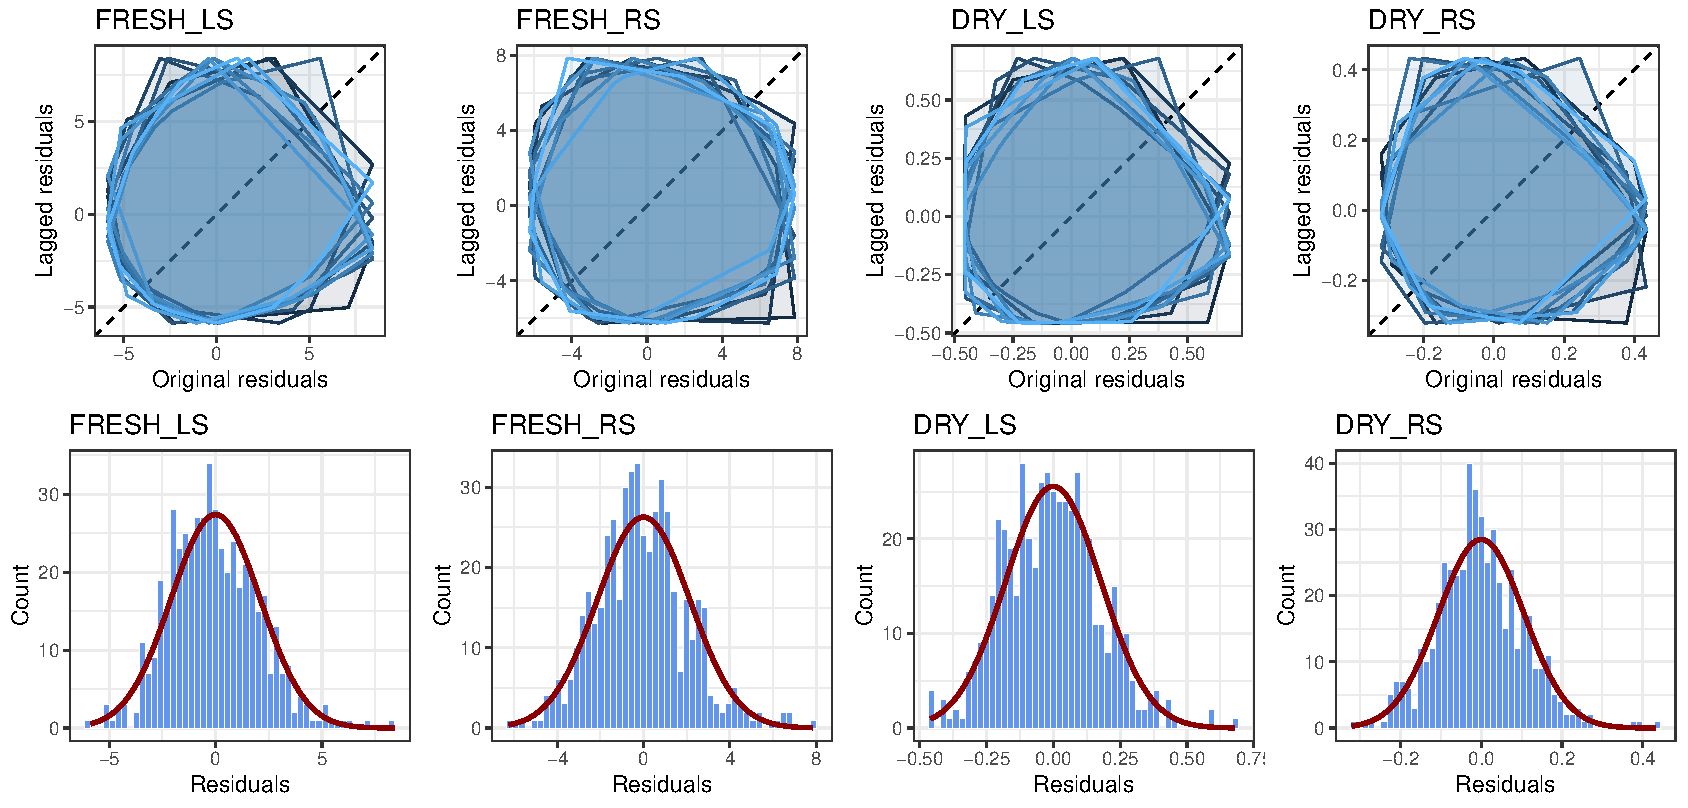
\includegraphics[width = 0.9\textwidth]{../../Figures/residuals_analysis_plot.pdf}
%%	\caption[Graphical analysis of the residuals og the SpATS model]{Graphical analysis of the residuals of the SpATS model for each variable: a convexhull of the lagplots of the residuals with different levels of lag (first row) and an histogram with a zero-mean, and same variance, normal distribution (second row).}
%%	\label{fig:residuals_analysis_plot}
%%\end{sidewaysfigure}

\section{Descriptive statistics}
\label{appendix:mean_std_table}

\begin{table}[ht]
\centering
\caption[Weighted mean and standard deviation for each genotype]{Weighted mean and standard deviation for each genotype. $\mathbf{DRY_{LS}}$ represents the dry weight of the leaf system; $\mathbf{DRY_{RS}}$, the dry weight for the root system; $\mathbf{FRESH_{LS}}$, the fresh weight for the leaf system and $\mathbf{FRESH_{RS}}$, the fresh weight for the root system. All the results are presented as mean $\pm$ standard deviation (g)}
\rowcolors{2}{gray!25}{white} 
\begin{tabular}{lrrrr}
  \toprule
Genotype & $DRY_{LS}$ & $DRY_{RS}$ & $FRESH_{LS}$ & $FRESH_{RS}$ \\ 
  \midrule
1 & 0.2267 $\pm$ 0.0869 & 0.2354 $\pm$ 0.0698 & 2.7231 $\pm$ 1.1612 & 3.4447 $\pm$ 1.4431 \\ 
  2 & 0.2113 $\pm$ 0.0993 & 0.1964 $\pm$ 0.06 & 2.4058 $\pm$ 1.254 & 2.2725 $\pm$ 1.1119 \\ 
  3 & 0.2132 $\pm$ 0.0747 & 0.1939 $\pm$ 0.0474 & 2.406 $\pm$ 1.0814 & 2.8146 $\pm$ 1.3663 \\ 
  4 & 0.227 $\pm$ 0.1148 & 0.1824 $\pm$ 0.0861 & 2.45 $\pm$ 1.5508 & 2.7773 $\pm$ 2.1926 \\ 
  5 & 0.2126 $\pm$ 0.113 & 0.1829 $\pm$ 0.0606 & 2.6521 $\pm$ 1.5044 & 3.0241 $\pm$ 1.7336 \\ 
  6 & 0.2024 $\pm$ 0.0739 & 0.1747 $\pm$ 0.051 & 2.4244 $\pm$ 1.1691 & 3.2168 $\pm$ 1.4545 \\ 
  7 & 0.126 $\pm$ 0.0441 & 0.1251 $\pm$ 0.0232 & 1.4118 $\pm$ 0.5677 & 1.5669 $\pm$ 0.5783 \\ 
  8 & 0.186 $\pm$ 0.0805 & 0.1798 $\pm$ 0.0567 & 2.3614 $\pm$ 1.1696 & 2.6894 $\pm$ 1.273 \\ 
  9 & 0.1559 $\pm$ 0.0865 & 0.2064 $\pm$ 0.0574 & 1.9704 $\pm$ 1.1782 & 2.3862 $\pm$ 1.3949 \\ 
  10 & 0.1885 $\pm$ 0.0875 & 0.1769 $\pm$ 0.0693 & 2.1228 $\pm$ 1.046 & 2.029 $\pm$ 1.0451 \\ 
  11 & 0.1789 $\pm$ 0.0811 & 0.1783 $\pm$ 0.0521 & 2.1608 $\pm$ 1.0747 & 2.339 $\pm$ 1.2172 \\ 
  12 & 0.1684 $\pm$ 0.0893 & 0.1469 $\pm$ 0.0417 & 2.0166 $\pm$ 0.9281 & 2.0985 $\pm$ 0.9015 \\ 
  13 & 0.1927 $\pm$ 0.0794 & 0.1639 $\pm$ 0.054 & 2.1326 $\pm$ 1.077 & 2.1176 $\pm$ 1.1582 \\ 
  14 & 0.2438 $\pm$ 0.1288 & 0.2173 $\pm$ 0.0796 & 3.0901 $\pm$ 1.6735 & 3.486 $\pm$ 1.8646 \\ 
  15 & 0.1175 $\pm$ 0.0885 & 0.2097 $\pm$ 0.0591 & 1.48 $\pm$ 1.2962 & 1.8417 $\pm$ 1.3372 \\ 
  16 & 0.3244 $\pm$ 0.1276 & 0.2208 $\pm$ 0.0879 & 3.7094 $\pm$ 1.8196 & 3.9028 $\pm$ 2.2598 \\ 
  17 & 0.2357 $\pm$ 0.1111 & 0.2019 $\pm$ 0.065 & 2.7519 $\pm$ 1.2418 & 2.8555 $\pm$ 1.4 \\ 
  18 & 0.1427 $\pm$ 0.039 & 0.1653 $\pm$ 0.0442 & 1.5621 $\pm$ 0.5627 & 1.7781 $\pm$ 0.8075 \\ 
  19 & 0.1785 $\pm$ 0.0505 & 0.1926 $\pm$ 0.04 & 2.0917 $\pm$ 0.7454 & 2.7726 $\pm$ 0.9668 \\ 
  20 & 0.1901 $\pm$ 0.0721 & 0.1506 $\pm$ 0.0497 & 2.0641 $\pm$ 0.9693 & 2.2429 $\pm$ 1.2908 \\ 
  21 & 0.1649 $\pm$ 0.0786 & 0.1859 $\pm$ 0.0329 & 1.9682 $\pm$ 0.8601 & 1.7689 $\pm$ 0.6407 \\ 
  22 & 0.1482 $\pm$ 0.0669 & 0.1508 $\pm$ 0.0296 & 1.522 $\pm$ 0.7799 & 1.793 $\pm$ 0.838 \\ 
  23 & 0.156 $\pm$ 0.04 & 0.1574 $\pm$ 0.0372 & 1.7621 $\pm$ 0.6537 & 1.9874 $\pm$ 0.9962 \\ 
  24 & 0.1668 $\pm$ 0.0827 & 0.1236 $\pm$ 0.0575 & 1.9357 $\pm$ 0.8693 & 2.0506 $\pm$ 1.2218 \\ 
  25 & 0.2013 $\pm$ 0.0856 & 0.1195 $\pm$ 0.0481 & 2.4338 $\pm$ 1.0937 & 1.9605 $\pm$ 1.1428 \\ 
  26 & 0.1463 $\pm$ 0.075 & 0.1573 $\pm$ 0.0365 & 1.7995 $\pm$ 1.1967 & 1.9256 $\pm$ 1.0053 \\ 
  27 & 0.1682 $\pm$ 0.0894 & 0.188 $\pm$ 0.0401 & 2.2662 $\pm$ 1.0855 & 2.3647 $\pm$ 1.0382 \\ 
  28 & 0.1753 $\pm$ 0.0865 & 0.2244 $\pm$ 0.066 & 2.0357 $\pm$ 1.0699 & 2.441 $\pm$ 1.1785 \\ 
  29 & 0.215 $\pm$ 0.0934 & 0.1823 $\pm$ 0.0663 & 2.4861 $\pm$ 1.3776 & 2.6743 $\pm$ 1.5787 \\ 
  30 & 0.1573 $\pm$ 0.0592 & 0.184 $\pm$ 0.0485 & 2.1033 $\pm$ 0.8712 & 2.51 $\pm$ 1.1265 \\ 
   \bottomrule
\end{tabular}
\label{tab:summary_table_all_variables}
\end{table}


\section{T-tests}
\label{appendix:t_test}
% Table generated by Excel2LaTeX from sheet 'Sheet1'
% Table generated by Excel2LaTeX from sheet 'Sheet1'
\begin{table}[htbp]
  \centering
  \caption[P-values resulting from the individual t-tests of the differences between means for all genotypes]{P-values resulting from the individual t-tests of the differences between means for all genotypes. All values inferior to 0.05 are colored in green, while value between 0.05 and 0.1 are in yellow and the rest is in red. P-value was not computed for genotype 30 since there were only 3 values available.}
    \begin{tabular}{lrrrr}
    \toprule
        Genotype  & \multicolumn{1}{l}{FRESH\_LS} & \multicolumn{1}{l}{FRESH\_RS} & \multicolumn{1}{l}{DRY\_LS} & \multicolumn{1}{l}{DRY\_LS} \\
          \bottomrule
    6     & \cellcolor[rgb]{ 1,  .922,  .612} \textcolor[rgb]{ .612,  .341,  0}{0,067045} & \cellcolor[rgb]{ .776,  .937,  .808} \textcolor[rgb]{ 0,  .38,  0}{8,18E-05} & \cellcolor[rgb]{ .776,  .937,  .808} \textcolor[rgb]{ 0,  .38,  0}{0,024774} & \cellcolor[rgb]{ .776,  .937,  .808} \textcolor[rgb]{ 0,  .38,  0}{0,000941} \\
    23    & \cellcolor[rgb]{ .776,  .937,  .808} \textcolor[rgb]{ 0,  .38,  0}{0,005072} & \cellcolor[rgb]{ .776,  .937,  .808} \textcolor[rgb]{ 0,  .38,  0}{0,009236} & \cellcolor[rgb]{ 1,  .922,  .612} \textcolor[rgb]{ .612,  .341,  0}{0,076901} & \cellcolor[rgb]{ .776,  .937,  .808} \textcolor[rgb]{ 0,  .38,  0}{0,036332} \\
    10    & \cellcolor[rgb]{ .776,  .937,  .808} \textcolor[rgb]{ 0,  .38,  0}{0,007526} & \cellcolor[rgb]{ .776,  .937,  .808} \textcolor[rgb]{ 0,  .38,  0}{0,001057} & \cellcolor[rgb]{ 1,  .78,  .808} \textcolor[rgb]{ .612,  0,  .024}{0,10752} & \cellcolor[rgb]{ 1,  .922,  .612} \textcolor[rgb]{ .612,  .341,  0}{0,054917} \\
    26    & \cellcolor[rgb]{ 1,  .922,  .612} \textcolor[rgb]{ .612,  .341,  0}{0,068053} & \cellcolor[rgb]{ .776,  .937,  .808} \textcolor[rgb]{ 0,  .38,  0}{0,029225} & \cellcolor[rgb]{ 1,  .922,  .612} \textcolor[rgb]{ .612,  .341,  0}{0,092141} & \cellcolor[rgb]{ .776,  .937,  .808} \textcolor[rgb]{ 0,  .38,  0}{0,007438} \\
    4     & \cellcolor[rgb]{ .776,  .937,  .808} \textcolor[rgb]{ 0,  .38,  0}{0,034853} & \cellcolor[rgb]{ .776,  .937,  .808} \textcolor[rgb]{ 0,  .38,  0}{0,024024} & \cellcolor[rgb]{ 1,  .78,  .808} \textcolor[rgb]{ .612,  0,  .024}{0,109144} & \cellcolor[rgb]{ .776,  .937,  .808} \textcolor[rgb]{ 0,  .38,  0}{0,032899} \\
    8     & \cellcolor[rgb]{ .776,  .937,  .808} \textcolor[rgb]{ 0,  .38,  0}{0,009049} & \cellcolor[rgb]{ .776,  .937,  .808} \textcolor[rgb]{ 0,  .38,  0}{0,00777} & \cellcolor[rgb]{ .776,  .937,  .808} \textcolor[rgb]{ 0,  .38,  0}{0,035141} & \cellcolor[rgb]{ 1,  .78,  .808} \textcolor[rgb]{ .612,  0,  .024}{0,201765} \\
    14    & \cellcolor[rgb]{ .776,  .937,  .808} \textcolor[rgb]{ 0,  .38,  0}{0,04338} & \cellcolor[rgb]{ .776,  .937,  .808} \textcolor[rgb]{ 0,  .38,  0}{0,023285} & \cellcolor[rgb]{ 1,  .78,  .808} \textcolor[rgb]{ .612,  0,  .024}{0,256493} & \cellcolor[rgb]{ 1,  .922,  .612} \textcolor[rgb]{ .612,  .341,  0}{0,09208} \\
    9     & \cellcolor[rgb]{ .776,  .937,  .808} \textcolor[rgb]{ 0,  .38,  0}{0,038485} & \cellcolor[rgb]{ .776,  .937,  .808} \textcolor[rgb]{ 0,  .38,  0}{0,039673} & \cellcolor[rgb]{ 1,  .78,  .808} \textcolor[rgb]{ .612,  0,  .024}{0,220818} & \cellcolor[rgb]{ 1,  .78,  .808} \textcolor[rgb]{ .612,  0,  .024}{0,123382} \\
    24    & \cellcolor[rgb]{ .776,  .937,  .808} \textcolor[rgb]{ 0,  .38,  0}{0,042817} & \cellcolor[rgb]{ .776,  .937,  .808} \textcolor[rgb]{ 0,  .38,  0}{0,015859} & \cellcolor[rgb]{ 1,  .78,  .808} \textcolor[rgb]{ .612,  0,  .024}{0,408412} & \cellcolor[rgb]{ 1,  .922,  .612} \textcolor[rgb]{ .612,  .341,  0}{0,079817} \\
    3     & \cellcolor[rgb]{ 1,  .922,  .612} \textcolor[rgb]{ .612,  .341,  0}{0,07032} & \cellcolor[rgb]{ .776,  .937,  .808} \textcolor[rgb]{ 0,  .38,  0}{0,020974} & \cellcolor[rgb]{ 1,  .78,  .808} \textcolor[rgb]{ .612,  0,  .024}{0,492672} & \cellcolor[rgb]{ 1,  .922,  .612} \textcolor[rgb]{ .612,  .341,  0}{0,060329} \\
    29    & \cellcolor[rgb]{ 1,  .922,  .612} \textcolor[rgb]{ .612,  .341,  0}{0,066428} & \cellcolor[rgb]{ 1,  .922,  .612} \textcolor[rgb]{ .612,  .341,  0}{0,055044} & \cellcolor[rgb]{ 1,  .78,  .808} \textcolor[rgb]{ .612,  0,  .024}{0,348994} & \cellcolor[rgb]{ 1,  .78,  .808} \textcolor[rgb]{ .612,  0,  .024}{0,183319} \\
    25    & \cellcolor[rgb]{ 1,  .922,  .612} \textcolor[rgb]{ .612,  .341,  0}{0,086712} & \cellcolor[rgb]{ .776,  .937,  .808} \textcolor[rgb]{ 0,  .38,  0}{0,013015} & \cellcolor[rgb]{ 1,  .78,  .808} \textcolor[rgb]{ .612,  0,  .024}{0,564199} & \cellcolor[rgb]{ 1,  .922,  .612} \textcolor[rgb]{ .612,  .341,  0}{0,091173} \\
    16    & \cellcolor[rgb]{ .776,  .937,  .808} \textcolor[rgb]{ 0,  .38,  0}{0,015628} & \cellcolor[rgb]{ .776,  .937,  .808} \textcolor[rgb]{ 0,  .38,  0}{0,002877} & \cellcolor[rgb]{ 1,  .78,  .808} \textcolor[rgb]{ .612,  0,  .024}{0,637848} & \cellcolor[rgb]{ 1,  .78,  .808} \textcolor[rgb]{ .612,  0,  .024}{0,164959} \\
    27    & \cellcolor[rgb]{ 1,  .922,  .612} \textcolor[rgb]{ .612,  .341,  0}{0,068433} & \cellcolor[rgb]{ .776,  .937,  .808} \textcolor[rgb]{ 0,  .38,  0}{0,001215} & \cellcolor[rgb]{ 1,  .78,  .808} \textcolor[rgb]{ .612,  0,  .024}{0,728604} & \cellcolor[rgb]{ .776,  .937,  .808} \textcolor[rgb]{ 0,  .38,  0}{0,036351} \\
    15    & \cellcolor[rgb]{ 1,  .78,  .808} \textcolor[rgb]{ .612,  0,  .024}{0,249287} & \cellcolor[rgb]{ 1,  .78,  .808} \textcolor[rgb]{ .612,  0,  .024}{0,264329} & \cellcolor[rgb]{ 1,  .78,  .808} \textcolor[rgb]{ .612,  0,  .024}{0,299309} & \cellcolor[rgb]{ 1,  .78,  .808} \textcolor[rgb]{ .612,  0,  .024}{0,383055} \\
    18    & \cellcolor[rgb]{ 1,  .78,  .808} \textcolor[rgb]{ .612,  0,  .024}{0,25502} & \cellcolor[rgb]{ 1,  .922,  .612} \textcolor[rgb]{ .612,  .341,  0}{0,054048} & \cellcolor[rgb]{ 1,  .78,  .808} \textcolor[rgb]{ .612,  0,  .024}{0,806946} & \cellcolor[rgb]{ 1,  .78,  .808} \textcolor[rgb]{ .612,  0,  .024}{0,14867} \\
    13    & \cellcolor[rgb]{ 1,  .78,  .808} \textcolor[rgb]{ .612,  0,  .024}{0,278165} & \cellcolor[rgb]{ 1,  .78,  .808} \textcolor[rgb]{ .612,  0,  .024}{0,130413} & \cellcolor[rgb]{ 1,  .78,  .808} \textcolor[rgb]{ .612,  0,  .024}{0,634507} & \cellcolor[rgb]{ 1,  .78,  .808} \textcolor[rgb]{ .612,  0,  .024}{0,287053} \\
    5     & \cellcolor[rgb]{ 1,  .78,  .808} \textcolor[rgb]{ .612,  0,  .024}{0,112019} & \cellcolor[rgb]{ .776,  .937,  .808} \textcolor[rgb]{ 0,  .38,  0}{0,047269} & \cellcolor[rgb]{ 1,  .78,  .808} \textcolor[rgb]{ .612,  0,  .024}{0,439077} & \cellcolor[rgb]{ 1,  .78,  .808} \textcolor[rgb]{ .612,  0,  .024}{0,742416} \\
    12    & \cellcolor[rgb]{ 1,  .78,  .808} \textcolor[rgb]{ .612,  0,  .024}{0,302533} & \cellcolor[rgb]{ 1,  .78,  .808} \textcolor[rgb]{ .612,  0,  .024}{0,792875} & \cellcolor[rgb]{ 1,  .922,  .612} \textcolor[rgb]{ .612,  .341,  0}{0,051195} & \cellcolor[rgb]{ 1,  .78,  .808} \textcolor[rgb]{ .612,  0,  .024}{0,271333} \\
    1     & \cellcolor[rgb]{ .776,  .937,  .808} \textcolor[rgb]{ 0,  .38,  0}{0,027344} & \cellcolor[rgb]{ .776,  .937,  .808} \textcolor[rgb]{ 0,  .38,  0}{0,004086} & \cellcolor[rgb]{ 1,  .78,  .808} \textcolor[rgb]{ .612,  0,  .024}{0,93751} & \cellcolor[rgb]{ 1,  .78,  .808} \textcolor[rgb]{ .612,  0,  .024}{0,512452} \\
    20    & \cellcolor[rgb]{ 1,  .78,  .808} \textcolor[rgb]{ .612,  0,  .024}{0,178574} & \cellcolor[rgb]{ 1,  .78,  .808} \textcolor[rgb]{ .612,  0,  .024}{0,110094} & \cellcolor[rgb]{ 1,  .78,  .808} \textcolor[rgb]{ .612,  0,  .024}{0,943514} & \cellcolor[rgb]{ 1,  .78,  .808} \textcolor[rgb]{ .612,  0,  .024}{0,447728} \\
    19    & \cellcolor[rgb]{ 1,  .78,  .808} \textcolor[rgb]{ .612,  0,  .024}{0,170245} & \cellcolor[rgb]{ .776,  .937,  .808} \textcolor[rgb]{ 0,  .38,  0}{0,038213} & \cellcolor[rgb]{ 1,  .78,  .808} \textcolor[rgb]{ .612,  0,  .024}{0,684042} & \cellcolor[rgb]{ 1,  .78,  .808} \textcolor[rgb]{ .612,  0,  .024}{0,87518} \\
    7     & \cellcolor[rgb]{ 1,  .78,  .808} \textcolor[rgb]{ .612,  0,  .024}{0,119486} & \cellcolor[rgb]{ .776,  .937,  .808} \textcolor[rgb]{ 0,  .38,  0}{0,017251} & \cellcolor[rgb]{ 1,  .78,  .808} \textcolor[rgb]{ .612,  0,  .024}{0,915835} & \cellcolor[rgb]{ 1,  .78,  .808} \textcolor[rgb]{ .612,  0,  .024}{0,878908} \\
    28    & \cellcolor[rgb]{ 1,  .78,  .808} \textcolor[rgb]{ .612,  0,  .024}{0,360779} & \cellcolor[rgb]{ 1,  .78,  .808} \textcolor[rgb]{ .612,  0,  .024}{0,127756} & \cellcolor[rgb]{ 1,  .78,  .808} \textcolor[rgb]{ .612,  0,  .024}{0,954177} & \cellcolor[rgb]{ 1,  .78,  .808} \textcolor[rgb]{ .612,  0,  .024}{0,606738} \\
    21    & \cellcolor[rgb]{ 1,  .78,  .808} \textcolor[rgb]{ .612,  0,  .024}{0,574376} & \cellcolor[rgb]{ 1,  .78,  .808} \textcolor[rgb]{ .612,  0,  .024}{0,503482} & \cellcolor[rgb]{ 1,  .78,  .808} \textcolor[rgb]{ .612,  0,  .024}{0,42371} & \cellcolor[rgb]{ 1,  .78,  .808} \textcolor[rgb]{ .612,  0,  .024}{0,570469} \\
    2     & \cellcolor[rgb]{ 1,  .78,  .808} \textcolor[rgb]{ .612,  0,  .024}{0,453042} & \cellcolor[rgb]{ 1,  .922,  .612} \textcolor[rgb]{ .612,  .341,  0}{0,077753} & \cellcolor[rgb]{ 1,  .78,  .808} \textcolor[rgb]{ .612,  0,  .024}{0,790318} & \cellcolor[rgb]{ 1,  .78,  .808} \textcolor[rgb]{ .612,  0,  .024}{0,828287} \\
    11    & \cellcolor[rgb]{ 1,  .78,  .808} \textcolor[rgb]{ .612,  0,  .024}{0,875426} & \cellcolor[rgb]{ 1,  .78,  .808} \textcolor[rgb]{ .612,  0,  .024}{0,772947} & \cellcolor[rgb]{ 1,  .78,  .808} \textcolor[rgb]{ .612,  0,  .024}{0,404975} & \cellcolor[rgb]{ 1,  .78,  .808} \textcolor[rgb]{ .612,  0,  .024}{0,179616} \\
    22    & \cellcolor[rgb]{ 1,  .78,  .808} \textcolor[rgb]{ .612,  0,  .024}{0,793643} & \cellcolor[rgb]{ 1,  .78,  .808} \textcolor[rgb]{ .612,  0,  .024}{0,55334} & \cellcolor[rgb]{ 1,  .78,  .808} \textcolor[rgb]{ .612,  0,  .024}{0,510492} & \cellcolor[rgb]{ 1,  .78,  .808} \textcolor[rgb]{ .612,  0,  .024}{0,40223} \\
    17    & \cellcolor[rgb]{ 1,  .78,  .808} \textcolor[rgb]{ .612,  0,  .024}{0,887499} & \cellcolor[rgb]{ 1,  .78,  .808} \textcolor[rgb]{ .612,  0,  .024}{0,192592} & \cellcolor[rgb]{ 1,  .78,  .808} \textcolor[rgb]{ .612,  0,  .024}{0,493846} & \cellcolor[rgb]{ 1,  .78,  .808} \textcolor[rgb]{ .612,  0,  .024}{0,835214} \\
    30    & . & . & . & . \\
    \midrule
    \end{tabular}%
  \label{tab:ind_geno_t_test_pval}%
\end{table}%




\section{Variance tables}
\subsection{SpATS variance table}
\label{appendix:tab_spats_variances}

\begin{table}[ht]
\centering
\rowcolors{2}{gray!25}{white}
\caption{Individual variances of all the components of the SpATS model.} 
\begin{tabular}{lrrrr}
  \toprule
 & FRESH\_LS & FRESH\_RS & DRY\_LS & DRY\_RS \\ 
  \midrule
$\mathbf{c}_{g}$ & 0.171 & 0.262 & 1.27$\times 10^{-3}$ & 6.9$\times 10^{-4}$ \\ 
  $\mathbf{c}_{v}$ & 3.24$\times 10^{-3}$ & 5.08$\times 10^{-3}$ & 1.95$\times 10^{-7}$ & 8.47$\times 10^{-17}$ \\ 
  $\mathbf{c}_{u}$ & 1.86$\times 10^{-4}$ & 2.25$\times 10^{-5}$ & 2.42$\times 10^{-7}$ & 3.93$\times 10^{-8}$ \\ 
  $f_{v}(\mathbf{v})$ & 2.2 & 11 & 1.06$\times 10^{-4}$ & 0.265 \\ 
  $f_{u}(\mathbf{u})$ & 2.75$\times 10^{-5}$ & 5.36$\times 10^{-5}$ & 5.4$\times 10^{-8}$ & 1.55$\times 10^{-8}$ \\ 
  $\boldsymbol{u} \odot h_{v}(\boldsymbol{v})$ & 5.60$\times 10^{-52}$ & 1.76$\times 10^{-38}$ & 1.51$\times 10^{-52}$ & 1.44$\times 10^{-13}$ \\ 
  $\boldsymbol{v} \odot h_{u}(\boldsymbol{u})$ & 1.81$\times 10^{-9}$ & 4.83$\times 10^{-4}$ & 6.75$\times 10^{-10}$ & 1.43$\times 10^{-6}$ \\ 
  $f_{u, v}(\boldsymbol{u}, \boldsymbol{v})$ & 0.398 & 0.252 & 6.13$\times 10^{-5}$ & 7.13$\times 10^{-4}$ \\ 
  $\epsilon$ & 4.707 & 5.014 & 0.03364 & 0.01219\\
   \bottomrule
\end{tabular}
\label{tab:spats_variances}
\end{table}

%\chapter{Hoagland solution}
%\label{appendix:hoagland}
%
%\rowcolors{2}{gray!25}{white}
%
%\captionsetup[table]{list=no}
%\begin{table}[hbtp]
%    \centering
%    \caption{Composition of the \textit{Hoagland} nutritive solution. The pH must be adjusted to 5.0 using \ch{HCl} 1\% before using.}
%    \label{tab:my_label}
%    \begin{threeparttable}
%    \begin{tabular}{>{\bfseries}p{4cm} p{4cm} p{4cm}}
%    \toprule
%        Components & \textbf{Concentration (g/L)} & \textbf{ml for 25L of solution}\tnote{1} \\
%    \midrule
%        2M \ch{KNO3} & 202 & 62.5 \\
%        2M \ch{Ca(NO3)2} x \ch{4 H2O}  & 472 & 62.5\\
%        2M \ch{MgSO4} x \ch{7 H2O} & 493 & 25\\
%        1M \ch{NH4NO3} & 80 & 25\\
%        Minors: \newline
%        \ch{H3BO3} \newline
%        \ch{MnCl2} x \ch{4 H2O} \newline
%        \ch{ZnSO4} x \ch{7 H2O} \newline
%        \ch{CuSO4} \newline
%        \ch{H3MoO4} x \ch{H2O} or \newline
%        \ch{Na2MoO4} x \ch{2 H2O} & 
%        ~    \newline
%        2.86 \newline
%        1.81 \newline
%        0.22 \newline
%        0.051 \newline
%        0.09 \newline 
%        0.12 & 
%        ~    \newline
%        ~    \newline
%        ~    \newline
%        25 \tnote{2} \\
%        1M \ch{KH2PO4} (ph to 6.0 with 3M \ch{KOH}) & 136 & 12.5\\
%        Iron (Sprint 138 iron chelate) & 15 & 75\\
%    \bottomrule
%    \end{tabular}
%    \begin{tablenotes}\footnotesize
%        \item[1] For a 1:1 solution to use with 25L of water.
%        \item[2] All the minors elements are grouped, in the right proportions, in a "minor" solution.
%    \end{tablenotes}
%    \end{threeparttable}
%\end{table}
%\captionsetup[table]{list=yes}

\chapter{Phenotyping platform information file}
\label{appendix:platform_info}
\clearpage
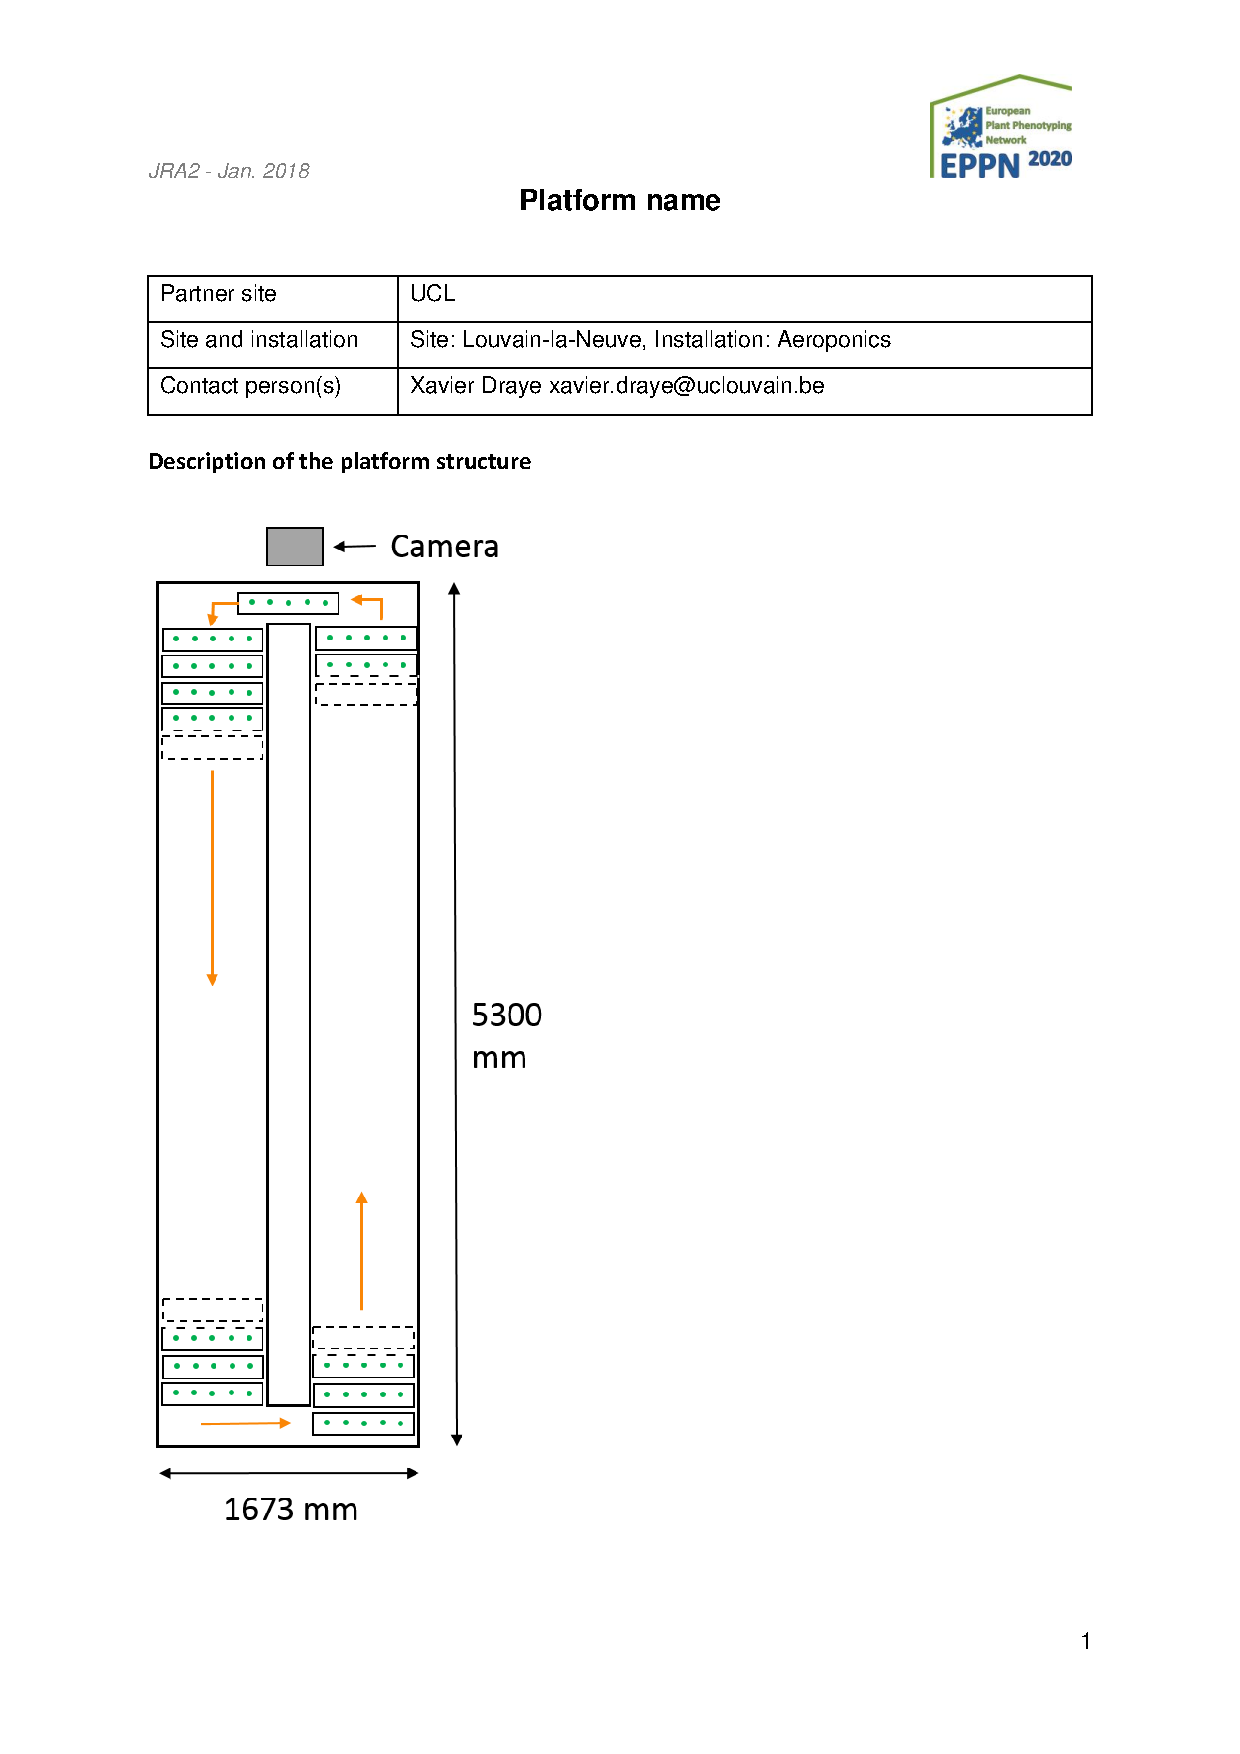
\includepdf[pages=-,pagecommand={},width=\textwidth]{extra/platform_info.pdf}

\end{appendices}

%% Back cover %%
% Back cover
\afterpage{\blankpage}
\newpage
\thispagestyle{empty}
\sffamily
%
\begin{textblock}{191}(113,-11)
{\color{blueline}\rule{160pt}{5.5pt}}
\end{textblock}
%
\begin{textblock}{191}(168,-11)
{\color{blueline}\rule{5.5pt}{59pt}}
\end{textblock}
%
\begin{textblock}{183}(-24,-11)
\textblockcolour{}
\flushright
\fontsize{7}{7.5}\selectfont
\textbf{Leuven Statistics Research Centre (LStat)}\\
Celestijnenlaan 200 B\\
3001 HEVERLEE, BELGI\"{E}\\
tel. +32 16 32 88 75 \\
https://lstat.kuleuven.be/contact\\
\end{textblock}
%
\begin{textblock}{191}(154,-7)
\textblockcolour{}
\includegraphics*[height=16.5truemm]{sedes}
\end{textblock}
%
\begin{textblock}{191}(-20,235)
{\color{bluetitle}\rule{544pt}{55pt}}
\end{textblock}
\end{document}